\documentclass[11pt,a4paper,oneside]{book}

%%%% PACKAGES WITH OPTIONS
\usepackage[english]{babel} % Language-specific hyphenation/splitting
\usepackage[small,bf,centerlast]{caption}[=v1] % Customise appearance of fig/table captions
\usepackage[Sonny]{fncychap} % Styles for chapter headers: Bjarne, Bjornstrup, Conny, Glenn, Lenny, Rejne and Sonny
\usepackage[T1]{fontenc} % Improved font encoding for better output, especially for accented characters
% \usepackage[inner=2.5cm,outer=2.5cm,vmargin=2.5cm]{geometry} % Set page margins
\usepackage[final]{graphicx} % Handles inclusion of images
\usepackage[UTF8]{inputenc} % Support for Latin-1 encoding (UTF-8 is generally preferred)\\
\usepackage[version=4]{mhchem} % Chemistry and isotopes with \ce{} (other option: 'chemformula' \ch{})
\usepackage[square,sort&compress,numbers]{natbib} % For formatted bibliographies with numeric citation styles
\usepackage[final]{pdfpages} % Inclusion of external PDF files
\usepackage{setspace} % Controls line spacing; "onehalfspacing" adds readability
\usepackage[separate-uncertainty=true]{siunitx} % Fancy display of SI units, can show uncertainty (e.g. \SI{1.54(6)}{\tesla} --> 1.54 ± 0.06 T)
\usepackage[dvipsnames]{xcolor} % Advanced color handling with named colors

%%%% PACKAGES WITHOUT OPTIONS
\usepackage{a4wide} % Adjusts margins for A4 paper (could conflict with "geometry")
%\usepackage{alphalph,cite} % Alphabetic-style labels
\usepackage{amsfonts}
\usepackage{amsmath} % Advanced math formatting and features
\usepackage{amssymb} % Additional math symbols
\usepackage{amsthm} % Environments like "proof"
\usepackage{bm} % Bold math symbols
\usepackage{cancel} % Strikethrough diagonal in math mode
\usepackage{changepage} % Enables adjustable margins within the document
\usepackage{color} % Basic color support (often superseded by "xcolor")
\usepackage{enumitem}
\usepackage{float} % Provides option [H] to floats
\usepackage[backref=none]{hyperref} % Creates hyperlinks and metadata in PDFs. Set backref=page to add back-references in bibliography.
\usepackage{ifthen} % If/then/else
\usepackage{listings} % Formats code snippets for programming examples
\usepackage{lmodern} % Modern font family with better scalability and appearance
\usepackage{longtable} % Tables that can span multiple pages
\usepackage{lscape} % Rotate content to landscape orientation
\usepackage{makecell} % Line breaks in table cells
\usepackage{makeidx} % Creates an index for the document
\usepackage[framemethod=TikZ]{mdframed} % Creates framed content with custom styles
\usepackage{microtype} % Enhances typographic appearance (e.g., kerning and justification)
\usepackage{nonfloat} % Prevents floating figures/tables for specific environments
\usepackage{pagecolor} % Sets background color of pages
\usepackage{physics2} % Simplifies common physics expressions and notation
\usepackage{ragged2e} % Provides \justifying command
\usepackage{soul} % For text decoration, e.g., underline (\ul{}), strikethrough (\st{}), highlighting...
% \usepackage{subcaption} % Subfigure captions
\usepackage{tikz}
\usepackage{titlesec} % Customises the format and spacing of section titles (e.g. \setcounter{secnumdepth} to make subsubsections numbered in chapters)
\usepackage{tocbibind} % Adds bibliography and table of contents to ToC
\usepackage{tocloft} % Customises the layout of the table of contents
\usepackage{upgreek} % Upright Greek letters
\usepackage{wasysym} % Many symbols
\usepackage{xfrac} % For diagonal fractions in text mode with \sfrac{}{}
\usepackage{xspace} % Automatically manages spaces after commands
\usepackage{xurl} % Better URL handling with line breaks

%%%% PACKAGES THAT MUST BE LOADED AFTER OTHERS
\usepackage[all]{hypcap} % [Requires "hyperref"] Ensures links to figures focus on the image, not the caption
\usepackage[capitalise]{cleveref} % [Requires "hyperref"] Intelligent cross-referencing

%%%% CREATE CUSTOM COMMANDS
% \definecolor{figcolor}{HTML}{F2F2FF}
\definecolor{figcolor}{HTML}{F2F2F2}
\definecolor{ugentblue}{RGB}{10,30,96}
\definecolor{lightblue}{HTML}{1E90FF} % C0
\definecolor{lightred}{HTML}{D62728} % C1
\definecolor{mplgrey}{gray}{0.5} % "grey" in matplotlib

\newcommand{\colorcode}{(Color code on page \pageref{colorcode}.)\xspace}

%% Index labels.
% To avoid multiply-defined labels, but allow multiple pages in the index, use e.g. \idx[nolabel]{...} after the first \idx{...}. 
\newcommand{\indexlabel}[2][]{\index{#2}\ifthenelse{\equal{#1}{nolabel}}{}{\label{#2}\label{#2s}}}
\newcommand{\idx}[2][]{\emph{#2}\indexlabel[#1]{#2}} %no xspace
\newcommand{\xlabel}[2][]{#2\indexlabel[#1]{#2}}
%% Index references.
\newcommand{\xref}[1]{\hyperref[#1]{#1}\xspace}
\newcommand{\xrefs}[2]{\hyperref[#2]{#1#2}\xspace} %% meervoud etc, add {s}
\newcommand{\link}[2]{\hyperref[#1]{#2}\xspace}

\newcommand{\jonathanskip}{\smallskip}
\newcommand{\numberthis}{\addtocounter{equation}{1}\tag{\theequation}} % Numbers a single line in a no-numbering multiline equation* or align*
\newcommand{\numeq}[2]{\stackrel{\scriptscriptstyle(\mkern-1.5mu#1\mkern-1.5mu)}{#2}} % Number above mathematical symbol (usage: \numeq{<eq_number>}{<symbol>})

%\newcommand{\debug}[1]{}
%\newcommand{\debug}[1]{{\tiny{(\pageref{#1})}}\normalsize}

\newcommand{\crefSubFigRef}[2]{\namecref{#1}~\hyperref[#1]{\ref{#1}#2}}
\newcommand{\ccite}[1]{Ref.~\cite{#1}} % Ref. [1] instead of [1]
\newcommand{\Py}{\xref{permalloy}}
%%vector
% \newcommand{\vc}[1]{\textbf{#1}}
\newcommand{\vc}[1]{\boldsymbol{\mathbf{#1}}} % Use this instead of \vb, which is deprecated anyway alongside the "physics" package
\newcommand{\circled}[1]{\raisebox{.5pt}{\textcircled{\raisebox{-.9pt} {#1}}}}
\newcommand{\sub}[1]{\ensuremath{_{\mathrm{#1}}}}
\newcommand{\super}[1]{\ensuremath{^{\mathrm{#1}}}}
\newcommand{\av}[1]{\langle #1 \rangle}
\newcommand{\sav}[1]{\langle\hspace{-0.4mm}\langle #1 \rangle\hspace{-0.4mm}\rangle}
%\newcommand{\sav}[1]{\left<\hspace{-0.4mm}\left< #1 \right>\hspace{-0.4mm}\right>}
\newcommand{\tpar}[1]{\frac{\partial #1}{\partial t}}%partial derivative to time
\newcommand{\tder}[1]{\frac{\mathrm{d} #1}{\mathrm{dt}}}%full derivative to time

\newcommand{\EB}{E_\mathrm{B}}
\newcommand{\EBeff}{\widetilde{\EB}}
\newcommand{\EBeffLeft}{\EBeff{}_{,\circlearrowleft}}
\newcommand{\EBeffRight}{\EBeff{}_{,\circlearrowright}}
\newcommand{\EEA}{E_\mathrm{EA}}
\newcommand{\EMC}{E_\mathrm{MC}}
\newcommand{\kB}{\ifmmode k_\mathrm{B} \else $k_\mathrm{B}$ \fi}
\newcommand{\kBT}{\ifmmode k_\mathrm{B}T \else $k_\mathrm{B}T$ \fi}
\newcommand{\clockwise}{\boldsymbol{\circlearrowright}}
\newcommand{\counterclockwise}{\boldsymbol{\circlearrowleft}}
\newcommand{\rmin}{r_\mathrm{min}}
\newcommand{\bigmu}{\makebox{\Large\ensuremath{\upmu}}}
\newcommand{\mavg}{m_\mathrm{avg}}
\newcommand{\qNN}[1][]{q_\mathrm{#1NN}} % Usage: \qNN, \qNN[2], ...

% \newcommand{\abs}[1]{\ensuremath{\left| #1 \right|}\xspace}
\newcommand{\bigsum}{\mathop{\scalebox{2}{\(\sum\)}}}
\newcommand{\bigprod}{\mathop{\scalebox{2}{\(\prod\)}}}
\newcommand{\diff}[2]{\frac{\partial #1}{\partial #2}}			    %% derivative
\newcommand{\dispdiff}[2]{{\partial #1}/{\partial #2}}			    %% derivative
\newcommand{\difff}[2]{\frac{\partial^2 #1}{\partial #2^2}}			%% second derivative
\newcommand{\ddt}[1]{\ensuremath{\partial #1 / \partial t}}
%\newcommand{\d}{\ensuremath{\mathrm{d}}}
\newcommand{\ddiff}[2]{\frac{\d #1}{\d #2}}
\newcommand{\lapl}{\ensuremath{{\Delta}}}
\newcommand{\eqdef}{\stackrel{\small{\mathrm{def}}}{=}}
\newcommand{\inprod}{\cdot}
\newcommand{\bcdot}{\boldsymbol{\cdot}}
\renewcommand{\quote}[1]{``#1''}
\newcommand{\etal}{\textit{et al.}\xspace}

\newcommand{\code}[1]{\textsf{#1}}
\newcommand{\shell}[1]{{\texttt{#1}}\smallskip\\}
\newcommand{\python}[1]{\lstinline{#1}}

\newcommand{\hide}[1]{}

\newcommand{\glijbaantje}[2]{\vspace{-0.5cm}\begin{flushright}{\textit{#1}\\--- #2\\}\vspace{0.5cm}\end{flushright}}
\newcommand{\publicatie}[1]{Material from this chapter has also been published in \cite{#1}.}

\newcommand{\mumax}{mumax\textsuperscript{3}\xspace}
\newcommand{\mumaxplus}{mumax\textsuperscript{+}\xspace}
\newcommand{\oommf}{\textsc{oommf}\xspace}
\newcommand{\nmag}{Nmag\xspace}
\newcommand{\hotspice}{\textsc{Hotspice}\xspace}
\newcommand{\spinengine}{SpinENGINE\xspace}

%%%% EXTRA SYMBOLS
\DeclareSymbolFont{extraitalic}      {U}{zavm}{m}{it}
\DeclareMathSymbol{\Qoppa}{\mathord}{extraitalic}{161}
\DeclareMathSymbol{\qoppa}{\mathord}{extraitalic}{162}
\DeclareMathSymbol{\Sampi}{\mathord}{extraitalic}{165}
\DeclareMathSymbol{\sampi}{\mathord}{extraitalic}{166}
\DeclareMathSymbol{\Stigma}{\mathord}{extraitalic}{167}
\DeclareMathSymbol{\stigma}{\mathord}{extraitalic}{168}

\newcommand{\eqn}[1]{equation \ref{#1}\xspace}
\newcommand{\secateur}[1]{section \ref{#1} (page \pageref{#1})\xspace}
\newcommand{\figuur}[1]{figure \ref{#1} (page \pageref{#1})\xspace}
\newcommand{\Figuur}[1]{Figure \ref{#1} (page \pageref{#1})\xspace}


\newcommand{\kolommen}[2]{
	\begin{minipage}{0.445\textwidth}
		#1
	\end{minipage}
	\begin{minipage}{0.445\textwidth}
		#2
	\end{minipage}
	\smallskip
}

\newcommand{\smallfig}[3]{
	\smallskip
	\begin{center}
		\includegraphics[width=#1\linewidth]{#2}\footnotesize{\\\textsf{(#3)}}
	\end{center}
	\smallskip
}

% 2 args: caption, tabular environment
% 1 optional arg: label
\newcommand{\xtable}[3][nolabel]{
	\jonathanskip\vspace{1em}
	\begin{tikzpicture}
		\node[rounded corners=10pt, fill=figcolor, inner sep=10pt] (figbox) {
			\begin{minipage}{0.955\linewidth}
		  		\centering
		  		\textsf{\tabcaption{#2\label{#1}}}
		  		{\sf
					#3
				}
			\end{minipage}
		};
	\end{tikzpicture}
	\jonathanskip\vspace{0.05cm}
}

% 2 args: filename, caption
% 1 optional arg: width
\newcommand{\xfig}[3][1]{
	\jonathanskip\vspace{1em}
	\begin{figure}[H] % Use the figure environment for compatibility
		\centering
		\begin{tikzpicture}
			\node[rounded corners=10pt, fill=figcolor, inner sep=10pt] (figbox) {
				\begin{minipage}{0.955\linewidth}
					\centering
					\includegraphics[width=#1\textwidth]{#2}
					\textsf{\caption{#3\label{#2}}}
				\end{minipage}
			};
		\end{tikzpicture}
	\end{figure}
	\jonathanskip\vspace{0.05cm}
}

% 5 args: filename1, caption1, filename2, caption2, overallcaption
% 1 optional arg: width of subfigures
\newcommand{\xfigs}[6][0.45]{
	\jonathanskip\vspace{1em}
	\begin{figure}[H] % Use the figure environment for compatibility
		\centering
		\begin{tikzpicture}
			\node[rounded corners=10pt, fill=figcolor, inner sep=10pt] (figbox) {
				\begin{minipage}{0.955\linewidth}
					\centering
					\begin{tabular}{cc}
						\small\parbox[c]{0.47\linewidth}{\centering\textsf{\textbf{(a)} #3}} & 
						\small\parbox[c]{0.47\linewidth}{\centering\textsf{\textbf{(b)} #5}}\normalsize \\
						\includegraphics[width=#1\linewidth]{#2} & 
						\includegraphics[width=#1\linewidth]{#4} \\
					\end{tabular}
					\textsf{\caption{#6\label{#2}}} % Ensure compatibility with hypcap
				\end{minipage}
			};
		\end{tikzpicture}
	\end{figure}
	\jonathanskip\vspace{0.05cm}
}

% 3 args: filename1, filename2, caption
% 1 optional arg: width of subfigures
\newcommand{\xfigsnocap}[4][0.45]{
	\jonathanskip\vspace{1em}
	\begin{figure}[H] % Use the figure environment for compatibility
		\centering
		\begin{tikzpicture}
			\node[rounded corners=10pt, fill=figcolor, inner sep=10pt] (figbox) {
				\begin{minipage}{0.955\linewidth}
					\centering
					\begin{tabular}{cc}
						\includegraphics[width=#1\linewidth]{#2} & 
						\includegraphics[width=#1\linewidth]{#3} \\
					\end{tabular}
					\textsf{\caption{#4\label{#2}}} % Ensure compatibility with hypcap
				\end{minipage}
			};
		\end{tikzpicture}
	\end{figure}
	\jonathanskip\vspace{0.05cm}
}

% 2 args: filename, caption
% 1 optional arg: width of subfigures
\newcommand{\sidefig}[3][1]{
	\jonathanskip\vspace{1em}
	\begin{figure}[H] % Use the figure environment for compatibility
		\centering
		\begin{tikzpicture}
			\node[rounded corners=10pt, fill=figcolor, inner sep=10pt] (figbox) {
				\begin{minipage}[c]{0.5\textwidth}
					\centering
					\includegraphics[width=#1\textwidth]{#2}
				\end{minipage}
				\begin{minipage}[c]{0.445\linewidth}
					\centering
					\textsf{\caption{\justifying #3\label{#2}}} % Ensure compatibility with hypcap
				\end{minipage}
			};
		\end{tikzpicture}
	\end{figure}
	\jonathanskip\vspace{0.05cm}
}


%%%% FIGURES BELOW HERE WERE NOT USED NOR ADJUSTED TO MODERN FORM (YET?)
\newcommand{\sidefigbig}[3][1]{
	\jonathanskip
	\colorbox{figcolor}{
	\begin{minipage}[c]{0.65\textwidth}
  		\centering
  		\includegraphics[width=#1\textwidth]{#2}
	\end{minipage}
	\begin{minipage}[c]{0.325\linewidth}
	 \textsf{\figcaption{#3\label{#2}}}
	\end{minipage}
	}
	\jonathanskip\vspace{0.05cm}
}

\newcommand{\makeshiftfig}[2]{
	\jonathanskip
	\colorbox{figcolor}{
		\begin{minipage}{\linewidth}
			\centering
			
			#1
			
			\textsf{\figcaption{#2}}
			
		\end{minipage}
	}
	\jonathanskip
}

\newcommand{\sidefigr}[3][1]{
	\jonathanskip
	\colorbox{figcolor}{
	\begin{minipage}[c]{0.455\linewidth}
	 \textsf{\figcaption{#3\label{#2}}}
	\end{minipage}
	\begin{minipage}[c]{0.5\textwidth}
  		\centering
  		\includegraphics[width=#1\textwidth]{#2}
	\end{minipage}
	}
	\jonathanskip\vspace{0.05cm}
}

\newcommand{\xfigssmallbig}[6][unused]{
	\jonathanskip
\colorbox{figcolor}{
	\begin{minipage}{0.955\linewidth}
  		\centering
		\begin{tabular}{cc}
		\small\parbox[c]{0.32\linewidth}{\textsf{\textbf{(a)} #3}} & \small\parbox[c]{0.62\linewidth}{\textsf{\textbf{(b)} #5}}\normalsize\\
		\includegraphics[width=0.3\linewidth]{#2} & \includegraphics[width=0.6\linewidth]{#4}\\
		\end{tabular}
		\textsf{\figcaption{#6\label{#2}}}
  	
	\end{minipage}
	
}\jonathanskip\vspace{0.05cm}}

\newcommand{\xfigssize}[8][unused]{
	\jonathanskip
\colorbox{figcolor}{
	\begin{minipage}{0.955\linewidth}
  		\centering
		\begin{tabular}{cc}
		\small\parbox[c]{#7\linewidth}{\textsf{\textbf{(a)} #3}} & \small\parbox[c]{#8\linewidth}{\textsf{\textbf{(b)} #5}}\normalsize\\
		\includegraphics[width=#7\linewidth]{#2} & \includegraphics[width=#8\linewidth]{#4}\\
		\end{tabular}
		\textsf{\figcaption{#6\label{#2}}}
  	
	\end{minipage}
	
}\jonathanskip\vspace{0.05cm}}

\newcommand{\xfigss}[8][0.45\textwidth]{
	%\\[\intextsep]
	\jonathanskip
	\colorbox{figcolor}{
	\begin{minipage}{\linewidth}
  		\centering
		\begin{tabular}{ccc}
		\small\parbox{0.3\linewidth}{\textsf{\textbf{(a)} #3}} & \parbox{0.3\linewidth}{\textsf{\textbf{(b)} #5}} & \parbox{0.3\linewidth}{\textsf{\textbf{(c)} #7}}\normalsize \\
		\includegraphics[width=0.3\linewidth]{#2} & \includegraphics[width=0.3\linewidth]{#4}& \includegraphics[width=0.3\linewidth]{#6}\\
		\end{tabular}
		\textsf{\figcaption{#8\label{#2}}}
  	
	\end{minipage}
	}
	\jonathanskip\vspace{0.05cm}
}

\newcommand{\xfigsss}[9]{
	%\\[\intextsep]
	\jonathanskip
\colorbox{figcolor}{
	\begin{minipage}{0.95\linewidth}
  		\centering
		\begin{tabular}{cccc}
		\small\parbox{0.23\linewidth}{\textsf{\textbf{(a)} #2}} & \small\parbox{0.23\linewidth}{\textsf{\textbf{(b)} #4}} & \small\parbox{0.23\linewidth}{\textsf{\textbf{(c)} #6}} & \small\parbox{0.23\linewidth}{\textsf{\textbf{(d)} #8}} \normalsize\\
		\includegraphics[width=0.23\linewidth]{#1} & \includegraphics[width=0.23\linewidth]{#3} & \includegraphics[width=0.23\linewidth]{#5}& \includegraphics[width=0.23\linewidth]{#7}\\
		\end{tabular}
		
		\textsf{\figcaption{#9\label{#1}}}
	\end{minipage}
	}
	\jonathanskip\vspace{0.05cm}
}

\newcommand{\moviefour}[5]{
	%\\[\intextsep]
	\jonathanskip
\colorbox{figcolor}{
	\begin{minipage}{0.95\linewidth}
  		\centering
			\includegraphics[width=0.21\linewidth]{#1} \hspace{0.1cm} \includegraphics[width=0.21\linewidth]{#2} \hspace{0.1cm} \includegraphics[width=0.21\linewidth]{#3} \hspace{0.1cm} \includegraphics[width=0.21\linewidth]{#4} \hspace{0.1cm}
		%\vspace{-1cm}
		\textsf{\figcaption{#5\label{#1}}}
	\end{minipage}
	}
	\jonathanskip\vspace{0.05cm}
}


\newcommand{\gridfour}[6]{
	%\\[\intextsep]
	\jonathanskip
\colorbox{figcolor}{
	\begin{minipage}{#6\linewidth}
  		\centering
			\includegraphics[width=0.46\linewidth]{#1} \hspace{0.1cm} \includegraphics[width=0.46\linewidth]{#2} \hspace{0.1cm}\\ \includegraphics[width=0.46\linewidth]{#3} \hspace{0.1cm} \includegraphics[width=0.46\linewidth]{#4} \hspace{0.1cm} 
		
		\textsf{\figcaption{#5\label{#1}}}
	\end{minipage}
	}
	\jonathanskip\vspace{0.05cm}
}

\newcommand{\cols}[2]{\parbox{0.5\linewidth}{#1}\parbox{0.5\linewidth}{#2}}

\newcommand{\phdtitle}{Modelling of Reservoir Computing in Perpendicular-Anisotropy Artificial Spin Ice}
\newcommand{\phdauthor}{Jonathan Maes}

%%%% PACKAGES SETUP COMMANDS
\graphicspath{{fig/}} % Package "graphicx"
\sisetup{ % Package "siunitx"
   detect-weight=true
}
\usephysicsmodule{ab,ab.legacy} % Package "physics2": needs to load modules explicitly to avoid namespace conflicts
\hypersetup{ % Package "hyperref": configures options for hyperlinks, bookmarks, and metadata in PDFs.
   plainpages=false,
   colorlinks=true,
   citecolor=gray,
   linkcolor=ugentblue,
   filecolor=black,
   urlcolor=blue!60!black,
   pdftitle={\phdtitle},
   pdfauthor={\phdauthor}
}
\urlstyle{same}
% \captionsetup{ % Package "caption": adjusts the appearance and formatting of captions.
%    width=.85\columnwidth,
%    %format=hang, % 'Figure n' in front of whole caption
%    labelsep=endash,
%    justification=centerlast,
%    labelfont={bf}
% }
\mdfsetup{ % Package "mdframed": margins, padding, and spacing for custom-framed environments.
   skipabove=\topskip,
   skipbelow=\topskip
}
\setstcolor{red} % Package "soul": set color for text highlighting or strikethrough effects.
\titleformat{\paragraph}[hang]{\normalfont\normalsize\bfseries}{\theparagraph}{1em}{}
\titlespacing*{\paragraph}{0pt}{3.25ex plus 1ex minus .2ex}{0.5em}
\newcolumntype{P}[1]{>{\RaggedRight\arraybackslash}p{#1}} % Package "array" & "ragged2e"
\setcounter{secnumdepth}{3} % For "titlesec" package (secnumdepth): adjusts the depth for numbered sections and subsections.
\setcounter{tocdepth}{1} % No excessive table of contents!
\raggedbottom


\setlength{\headheight}{13.6pt} 


%%%% DEFINE BOXED ENVIRONMENTS WITH MDFRAMED PACKAGE
%% Algorithm
\mdfdefinestyle{algorithmstyle}{%
	roundcorner=10pt,
	backgroundcolor=figcolor,
	frametitlebackgroundcolor=gray!30,
	linecolor=gray!50, linewidth=0pt,
	frametitlerule=false,%
	innertopmargin=\topskip,
	innerbottommargin=\topskip,
	subtitleaboveline=true,
	subtitlebackgroundcolor=gray!10,
	%topline=false,
	%bottomline=false,
}
\mdtheorem[style=algorithmstyle]{algorithm}{Algorithm}

%%%% SETUP HEADER
\usepackage{fancyhdr}
\pagestyle{fancy}
\fancyhf{}
\fancyhf[HL]{\nouppercase{{\textsf{\jonathan}}}}  % Links in header het hoofdstuk,
\fancyhf[HR]{\textsf\textbf{{\thepage}}} 						% Rechts het paginanummer.


%%%% CODE HIGHLIGHTING
\definecolor{Code}{rgb}{0,0,0} 
\definecolor{Decorators}{rgb}{0.5,0.5,0.5} 
\definecolor{Numbers}{rgb}{0.5,0,0} 
\definecolor{MatchingBrackets}{rgb}{0.25,0.5,0.5} 
\definecolor{Keywords}{rgb}{0,0,1} 
\definecolor{self}{rgb}{0,0,0} 
\definecolor{Strings}{rgb}{0,0.63,0} 
\definecolor{Comments}{rgb}{0,0.63,0} 
\definecolor{Backquotes}{rgb}{0,0,0} 
\definecolor{Classname}{rgb}{0,0,0} 
\definecolor{FunctionName}{rgb}{0,0,0} 
\definecolor{Operators}{rgb}{0,0,0} 
\definecolor{Background}{rgb}{0.98,0.98,0.98} 
\lstset{
   language=Python,
   breakatwhitespace=false,
   breaklines=true,
   numbers=left, 
   numberstyle=\footnotesize\color{gray}, 
   numbersep=1em, 
   xleftmargin=1em, 
   framextopmargin=2em, 
   framexbottommargin=2em, 
   showspaces=false, 
   showtabs=false, 
   showstringspaces=false, 
   frame=l, 
   tabsize=4,
   basicstyle=\ttfamily\small\setstretch{1}, 
   backgroundcolor=\color{Background},
   commentstyle=\color{Comments}\slshape,
   stringstyle=\color{Strings},
   keywordstyle={\color{Keywords}\bfseries}, 
   keywordstyle={[2]\color{Decorators}\slshape}, 
   emph={self}, 
   emphstyle={\color{self}\slshape}
}

\makeindex
\hyphenation{sen-tence}


%% for b5
%\makeatletter
%\setlength{\oddsidemargin}{7.029mm}
%\setlength{\evensidemargin}{7.029mm}
%\addtolength{\evensidemargin}{21.5mm}
%\setlength{\textheight}{20cm}
%\setlength{\abovecaptionskip}{4pt}
%\makeatother



\begin{document}
\hypersetup{breaklinks=true}
\setlength{\parindent}{0cm}

\frontmatter
\newcommand{\jonathan}{\leftmark}

%\includepdf{fig/coverfig/frontpage}

\thispagestyle{empty}


%\includegraphics[width=22cm]{fig/coverfig/frontpage}\\
 
\fontsize{12pt}{14pt}\selectfont
 
\vspace*{-1.5cm}

\noindent\makebox[\textwidth]{\hfill
\includegraphics[width=11cm]{cover/ugentbalk_2022.png}\hfill}

\begin{center}
    \vspace{0.5cm}

    \fontsize{28pt}{28pt}\selectfont
    %\fontsize{17.28pt}{21pt}\selectfont
    \textcolor{ugentblue}{\textsc{Modelling of\\reservoir computing in\\perpendicular-anisotropy\\artificial spin ice}}\\
\end{center}
\vspace{0.0cm}
\fontseries{m}
\fontsize{12pt}{14pt}\selectfont
\vfill

\vspace*{1cm}
\begin{center}
	\centerline{
		\hspace{-.7em}
		\begin{tikzpicture}
			\node[anchor=south west,inner sep=0] (image) at (0,0) {\includegraphics[width=0.95\paperwidth]{cover/OOP_Relaxation.pdf}};
			\fadenode[70pt]{image}
		\end{tikzpicture}
	}
\end{center}
%\newline\null

\vspace*{0cm}
\fontsize{17.28pt}{21pt}\selectfont
\null\hfill \textbf{\textcolor{ugentblue}{\phdauthor}}\hspace*{3.0cm}\\
 
%\vspace{0.5cm}
\fontsize{12pt}{14pt}\selectfont

\newpage

\thispagestyle{empty}
%\noindent
%\includegraphics[width=22cm]{fig/coverfig/frontpage}\\

\fontsize{12pt}{14pt}\selectfont

\vspace*{-1.5cm}
%\includegraphics[width=\textwidth]{ugentbalk} \hspace{1cm} %\includegraphics[height=3cm]{mpilogo}
%\noindent\makebox[\textwidth]{\hfill\includegraphics[width=14cm]{cobined.png} }
\noindent\makebox[\textwidth]{\hfill
\includegraphics[width=12.5cm]{cover/ugentbalk_2022.png}\hfill}
\vspace{0.0cm}
\fontsize{20pt}{20pt}\selectfont
\begin{center}
{\textsc{\phdtitle}}\\
\end{center}

\fontsize{16pt}{16pt}\selectfont

\null\hfill Doctoral thesis\\
\null\hfill by \phdauthor\\
\vfill
\fontseries{m}
\fontsize{12pt}{14pt}\selectfont
Thesis submitted to obtain the degree of\\
Doctor of Science: Physics\\
\newline
Public defense: 4th of September, 2025 at\\
Department of Solid State Sciences\\
Faculty of Sciences\\
Ghent University\\


\fontsize{10pt}{12pt}\selectfont
\textbf{Promotors:}\\
Prof. dr. Bartel Van Waeyenberge (promotor)\hfill Ghent University, Belgium\\
Prof. dr. Jonathan Leliaert (co-promotor)\hfill Ghent University, Belgium\\
\newline
\textbf{Examination Commission:}\\
Prof. dr. ir. M. Boone (chair)\hfill Ghent University, Belgium\\
Prof. dr. J. Ryckebusch\hfill Ghent University, Belgium\\
Prof. dr. E. Folven\hfill Norges Teknisk-Naturvitenskapelige Universitet, Norway\\%Norwegian University of Science and Technology, Norway\\
Dr. J. Joos\hfill Ghent University, Belgium\\
Dr. A. Hrabec\hfill Eidgen\"ossische Technische Hochschule Z\"urich, Switzerland\\%Federal Institute of Technology Zurich, Switzerland\\

\newpage

\newpage
\thispagestyle{empty}
\null
\newpage

\clearpage
\thispagestyle{empty}


\chapter*{Acknowledgements}
I acknowledge thee. % TODO
\clearpage


%%%% TABLE OF CONTENTS (on one page)
\begingroup
\makeatletter
% Redefine the \chapter* header macro to remove vertical space
\def\@makeschapterhead#1{%
%\vspace*{50\p@}% Remove the vertical space
{\parindent \z@ \raggedright
\normalfont
\interlinepenalty\@M
\Huge \bfseries  #1\par\nobreak
\vskip 40\p@
   }}
\makeatother

\fontsize{12pt}{15pt}\selectfont
\tableofcontents
\fontsize{12pt}{14pt}\selectfont
\endgroup

\renewcommand{\baselinestretch}{1.1} 	  % De interlinie afstand wat vergroten.
\small\normalsize                        % Nodig om de baselinestretch goed te krijgen.

\mainmatter

\chapter*{Samenvatting (in Dutch)}\label{sec:Preface_NL}
\markboth{Samenvatting (in Dutch)}{Samenvatting (in Dutch)} % For headers in fncychap
\addcontentsline{toc}{chapter}{\nameref{sec:Preface_NL}}
In onze huidige samenleving zijn computers alomtegenwoordig.
Oorspronkelijk werden zij ingezet voor taken die exact uitvoerbaar waren via voorgeprogrammeerde wiskundige operaties, denk bijvoorbeeld aan het verwerken van gestructureerde data, het ondersteunen van het internet, en het uitvoeren van simulaties.
Sinds de opkomst van machinaal leren is hun scala aan mogelijke toepassingen uitgebreid tot veel complexere taken, met als meest recente voorbeeld de grote taalmodellen die ondertussen wijdverspreid zijn.
%Voor het trainen van moderne artifici\"ele systemen, zoals neurale netwerken, is echter een enorme hoeveelheid data nodig.
Het is echter inherent ineffici\"ent om dergelijke modellen te implementeren op conventionele hardware, aangezien de gebruikte algoritmes door vele abstractielagen worden gescheiden van de onderliggende transistor-gebaseerde hardware.
Hierdoor is er veel interesse ontstaan voor alternatieve rekenconcepten, onder andere ook door de gelimiteerde schaalbaarheid van transistoren en de scheiding tussen geheugen en rekenkracht in de traditionele von Neumann computerarchitectuur.
E\'en zulk concept is neuromorphic computing (neuromorfisch rekenen), waarbij men deze artifici\"ele scheidingen wil aanpakken door de synaptische interconnectiviteit van een biologisch brein na te bootsen, waar geheugen en rekenkracht samenvallen.
Een interessant onderzoeksdomein binnen deze context is in-materia computing, waarbij men zich afvraagt welke berekeningen een fysisch materiaal van nature uitvoert en hoe deze kunnen worden benut.
Op deze manier kunnen veel effici\"entere systemen worden bedacht door de vele abstractielagen in conventionele computers te vermijden. \\ % In plaats van wiskundige berekeningen op te leggen aan een fysisch object, zoals tot nu toe gedaan met schakelingen van transistoren.

Op de kruising tussen neuromorphic computing en in-materia computing bevindt zich het zogeheten reservoir computing (RC).
Hierbij wordt een niet-lineair dynamisch systeem met vervagende geheugenwerking --- het zogeheten ``reservoir'' --- gebruikt als zwarte doos.
Wanneer het reservoir verstoord wordt door een inputsignaal, genereert het een complexe dynamische respons.
Hierdoor kunnen de inputgegevens eenvoudiger worden verwerkt: het volstaat om een enkele lineaire transformatie te trainen op deze multidimensionale respons (zonder de eigenschappen van het reservoir aan te moeten passen), aangezien de niet-lineaire transformatie door het reservoir zelf wordt voorzien. 
Opmerkelijk is dat vele fysische media, gaande van een emmer water tot supergeleidende elektronica, de benodigde eigenschappen (niet-lineariteit, vervagend geheugen en hoge dimensionaliteit) van nature bezitten, waardoor zij direct als reservoirs kunnen gebruikt worden.
Dit zorgt voor een veel kortere trainingstijd en lager energiegebruik dan conventionele neurale netwerken, aangezien een deel van de berekening wordt uitbesteed aan het fysische substraat. \par
Het onderzoek dat in deze thesis wordt voorgesteld maakte deel uit van het Europese ``\spinengine'' project, dat zich specifiek toespitste op het gebruik van ensembles van nanomagneten voor reservoir computing.
Bijzondere aandacht ging naar artificieel spin-ijs (ASI), gezien dit soort systeem een sterk niet-lineaire respons genereert, terwijl zeer weinig energie verloren gaat tijdens het verwerken van informatie.
ASI bestaat uit een geordend rooster van interagerende bistabiele nanomagneten, waarvan de magnetisatierichting kan wisselen tussen de twee stabiele toestanden onder invloed van nabije magneten of thermische fluctuaties.
Uit concurrerende lokale interacties onstaat emergente dynamica, wat toelaat om ASI te gebruiken als fysisch reservoir.
Deze thesis richt zich specifiek op ASI met een magnetisatie uit het vlak: dergelijke systemen zijn extra aantrekkelijk aangezien er effici\"ente input- en uitleesmethoden voor bestaan.
Alle voorgaande concepten worden in meer detail ge\"introduceerd in hoofdstuk~\ref{ch:Introduction}. \\
%Het doel van deze thesis is te onderzoeken hoe verticaal gemagnetiseerd ASI ingezet kan worden voor reservoir computing.
%Aangezien een experimentele verkenning van de enorme ontwerpruimte van deze systemen tijdrovend zou zijn, is er geopteerd om een simulatie­-toolkit te ontwikkelen die deze vragen snel en flexibel kan beantwoorden. \\

Hoofdstuk~\ref{ch:Hotspice} stelt de open-source \hotspice Monte Carlo-simulator voor, die de dynamica van ASI simuleert met als doel om reservoir computing-strategie\"en te evalueren en optimale systeemparameters te bepalen.
Er wordt een Ising-achtig model gebruikt: elke magneet in het ASI wordt voorgesteld als een punt-dipool die kan wisselen tussen twee stabiele toestanden.
Verschillende verbeteringen op dit model worden voorgesteld, waarvan de nauwkeurigheid vervolgens wordt vergeleken. % met betrekking tot de simulatie van het dynamische gedrag van ASI.
Deze richten zich op drie aspecten van de simulatie:
\begin{itemize}[noitemsep,nolistsep] % With enumitem package
	\item het in rekening brengen van de eindige grootte van nanomagneten voor de berekening van onderlinge magnetostatische interacties,
	\item de afschatting van de effectieve energiebarri\`ere die de twee stabiele toestanden van een nanomagneet scheidt,
	\item het gebruikte Monte Carlo spin-flip-algoritme voor het simuleren van systeemdynamica.
\end{itemize}
In de tweede helft van het hoofdstuk worden implementatiedetails besproken, met een focus op de berekening van de magnetostatische interactie tussen alle magneten door middel van op voorhand berekende convolutiematrices.
Vervolgens wordt de effici\"entie van de simulator ge\"evalueerd, waarbij een methode wordt voorgesteld om de Monte Carlo-simulatie te versnellen door meerdere magneten tegelijk van magnetisatierichting te laten wisselen binnen \'e\'en simulatiestap.
De correcte werking van de software wordt daarna geverifieerd aan de hand van enkele analytisch oplosbare systemen.
Het hoofdstuk eindigt tenslotte met een vergelijking tussen simulaties en enkele eerder gepubliceerde experimenten, aan de hand waarvan de accuraatheid van de verschillende modelverbeteringen kan worden geanalyseerd. \\

In hoofdstuk~\ref{ch:Applications} wordt deze \hotspice simulator ingezet om de reservoir computing-prestaties van zowel thermisch actief als bevroren verticaal-gemagnetiseerd ASI te evalueren.
Het gedrag van deze systemen wordt grotendeels bepaald door de wisselwerking tussen verschillende energiebijdragen, zoals de loodrechte magnetische anisotropie en de vorm-anisotropie van elke nanomagneet.
Door een zorgvuldige keuze van systeemparameters kan thermisch actief ASI verkregen worden, dat spontaan richting de grondtoestand evolueert over een zekere tijdspanne.
Enkele parameters, zoals de magnetostatische koppeling tussen naaste buren en de netto loodrechte anisotropie, hebben een sterke impact op deze evolutie naar de grondtoestand.
Na het effect van deze parameters te analyseren, worden hun waarden bepaald voor een experimenteel vervaardigd ASI door simulaties te vergelijken met het experimenteel geobserveerde relaxatieproces. \par
Hierop voortbouwend wordt dit relaxatieproces benut voor reservoir computing.
De prestaties van dit thermisch active ASI worden beoordeeld op basis van zijn performantie op twee specifieke taken.
Eerst wordt de niet-lineariteit van het reservoir ge\"evalueerd door het een signaaltransformatie te laten uitvoeren.
Vervolgens wordt de geheugencapaciteit getest, door het reservoir de chaotische Mackey-Glass oscillator te laten voorspellen.
Aangezien thermisch actief ASI moeilijk te vervaardigen is, richt het laatste deel van dit hoofdstuk zich op bevroren ASI.
In tegenstelling tot thermisch actieve systemen kan bij bevroren ASI geen globale input worden toegepast, aangezien deze niet spontaan de grondtoestand kan bereiken.
In plaats daarvan wordt een methode ontwikkeld waarbij elke inputcyclus uit twee aparte stappen bestaat, hetgeen gecontroleerde domeinmuurpropagatie mogelijk maakt.
Hierdoor wordt de domeindynamica benut, wat de prestaties van het reservoir verbetert. \\

De belangrijkste resultaten van deze voorbije hoofdstukken worden tenslotte samengevat in hoofdstuk \ref{ch:Conclusion}, waarna deze thesis wordt afgesloten met een algemene beoordeling van de bekomen resultaten en een blik op toekomstig onderzoek.
\cleardoublepage
\chapter*{Preface}
% TODO END: write preface

This thesis is about ... \\

\cref{ch:Introduction} introduces several key concepts ... \\

\cref{ch:Hotspice} presents the open-source \hotspice Monte Carlo simulator for artificial spin ice (ASI), developed with the intent to evaluate reservoir computing strategies and to determine optimal system parameters.
It uses an Ising-like model: each magnet in the ASI is represented by a point dipole that can switch between two stable states.
Several model variants are presented, whose accuracy in simulating the behaviour of ASI is then compared and discussed.
These variants explore three key aspects of the simulation:
\begin{itemize}[noitemsep,nolistsep] % With enumitem package
	\item the choice of Monte Carlo spin-flip algorithm for simulating system dynamics,
	\item accounting for the finite size of magnets when calculating magnetostatic interactions,
	\item estimating the effective energy barrier that separates the stable states of a nanomagnet.
\end{itemize}
In the second half of the chapter, implementation details are discussed, in particular the calculation of the magnetostatic interaction between all magnets, alongside other strategies to improve performance of the Monte Carlo simulation.
The chapter ends by briefly verifying the software, through comparison of simulations against analytical solutions for several solvable systems. \\

In \cref{ch:Applications}, ... \\

In \cref{ch:Conclusion} ...
\cleardoublepage
\chapter{Introduction}\label{ch:Introduction}
\glijbaantje{It is important to draw wisdom from many different places.\\If we take it from only one place, it becomes rigid and stale.}{Uncle Iroh}
%\glijbaantje{If a machine is expected to be infallible then it cannot also be intelligent.}{Alan Turing}
% TODO: write CMOS instead of or alongside "transistor"

This introduction opens with the broader context and motivation for the research presented in this thesis.
We then introduce the physical reservoir computing paradigm and the key metrics used to quantify performance.
Since we focus on magnetic reservoirs,~\cref{sec:1:Nanomagnetism} describes the fundamentals of nanomagnetism and the physical phenomena that enable efficient input and readout.
Next, we turn to magnetic reservoirs, in particular artificial spin ice, before concluding with a brief description of simulation techniques suitable for these systems.

\section{Context}\label{sec:1:Context}
We live in a society where computers are ubiquitous. % and indispesable.
They have been used for a wide variety of applications, like scientific simulations, graphics rendering, processing well-structured data, running the internet\dots\,
Conventional computers --- consisting of transistors arranged into logic gates --- are well suited for such tasks which require exact mathematical operations to be executed.
However, our world provides many challenging tasks that can not be captured by such simple, exact sets of predefined rules.
The archetypical example of this is driving a car, but this extends far into other complex tasks that are often thought of as requiring some degree of ``intelligence'' --- whatever that word may entail exactly. \par
The field of \idx{machine learning} aims to tackle these rather complex tasks using artificial systems, the most prevalent of which nowadays are \xref{artificial neural networks} that take inspiration from the synaptic connections in a biological brain.
Over the years, neural networks have advanced significantly, most recently evidenced by the rise of large language models which have already had a broad societal impact~\cite{ImprovingLanguageGPT,GPT-4}.
However, training these systems to the point where they can perform any of the aforementioned tasks at a decent level requires vast amounts of data to fine-tune their ever increasing number of internal parameters --- accompanied by an unsustainably rising energy cost~\cite{QuantumNeuromorphicOpportunities,BLOOM_CarbonFootprint_176Bparam}.
This stands in stark contrast to biological brains, which are capable of learning patterns based on a far more limited set of data, while consuming orders of magnitude less power than an artificial system of equivalent computational capability~\cite{NeuromorphicSpintronics}.
Furthermore, running such neural networks on conventional hardware is encountering limits: to increase performance, the number of trainable parameters is rapidly being increased, but transistor scaling and power density limitations make it hard for hardware to keep up. % TODO REF
Hence, while advances in training algorithms and the ever increasing wealth of available data create ever more potent machine learning systems, the underlying approach is leading to a bottleneck. \par
Several factors that contribute to this bottleneck are often quoted in the context of neural networks or other machine learning algorithms running on conventional hardware:
\begin{itemize} % TODO: more references for these bullet points
	\item Conventional hardware uses transistors to perform logical operations.
	The ever increasing computational demands have driven \xlabel{Moore's law}, which states that the number of transistors on a chip doubles every couple of years.
	However, this scaling law appears untenable as transistors approach nanometre scales.
	Relatedly, \xlabel{Dennard scaling} initially allowed the power density of chips to remain roughly constant during this downscaling, but current leakage has inevitably led to increased power dissipation over the past two decades.
	In an attempt to patch this, multi-core processing has become prevalent, but the high power density still limits the number of cores that can operate simultaneously without overheating. % This results in so-called areas of ``dark silicon'' that are unused at a given instant.
	Thus, new kinds of energy-efficient hardware need to be explored.
	\item Conventional computers are built according to the von Neumann architecture, where computation (CPU) is separated from memory (RAM).
	However, transferring information from memory to the processing unit wastes a lot of time and energy, leading to the infamous \idx{von Neumann bottleneck}~\cite{TaskAdaptivePRC}.
	The separation between memory and processing is not fundamentally required: biological brains in the natural world exhibit no such divide as they use a vast network of interconnected neurons, yet they are nonetheless capable of learning, processing and retaining information.
	The field of \idx{in-memory computing} concerns itself with bridging this divide in artificial systems.
	\item Artificial neural networks, like any other machine learning system implemented on conventional hardware, are abstracted far away from the physical domain~\cite{RC_ASI}.
	Most advancements arise from improving their algorithms, but these have to be run on a particular (e.g., von Neumann) computer architecture made up of circuits that handle information encoded by physical devices like transistors~\cite{RC_SuperconductingElectronics}.
	These many layers of abstraction render this approach inherently inefficient, as it does not directly exploit the physical properties of the constituent materials for computation~\cite{RC_ASI}.
\end{itemize}
These various drawbacks of current implementations have become more noticeable over the past decade, as portrayed in~\cref{fig:1:Ngram}.
This has led to the advent of \idx{neuromorphic computing} --- a field of research at the intersection of biology, computer science and physics --- which takes inspiration from the brain to develop more efficient hardware for processing complex data in parallel.
While artificial neural networks are indeed inspired by the brain, their implementation on conventional hardware is typically not considered part of neuromorphic computing, though approaches to implement neural networks on more efficient unconventional hardware are. % rather than applying algorithms on existing transistor-based hardware.
Note that neuromorphic computing does not seek to replace conventional computing: the latter will always find applications in systems that require absolute precision. % think of physical simulations, the transmission of data, or something as common as rendering an image on a screen.
Neuromorphic computing, on the other hand, does not seek exact solutions; in the words of Alan Turing, ``if a machine is expected to be infallible then it cannot also be intelligent.''
%This paradigm shift opens the door to innovative approaches for tackling computational challenges, particularly in areas like real-time sensing, pattern recognition, and prediction.
%Noise can explore a high dimensional landscape related to cost function by escaping local minima.

\vspace{-1.5em}
\sidefig[0.6]{1_Introduction/Ngrams.pdf}{
	\label{fig:1:Ngram}
	Popularity of various key concepts from the year 2000 onwards.
	The surge in popularity of alternative brain-inspired and physical computing methods coincides with raising concerns related to the usage of conventional hardware.
	Data provided by the \href{https://books.google.com/ngrams/graph?content=Neuromorphic computing,Reservoir computing,In-memory computing,von Neumann bottleneck,Dennard scaling,Material computation&year_start=2000&year_end=2022&corpus=en&smoothing=3&case_insensitive=false}{Google Books Ngram viewer} throughout the English corpus, smoothed over a 3-year period.
	\newline
}
\vspace{-1em}

A related concept is \xlabel{material computation}~\cite{NeglectedPillar}, which goes one step further: its goal is to find ways to exploit the inherent computing power present in physical substrates.
Whereas classical computing uses a top-down approach where mathematics is imposed onto a physical material --- for instance to construct logic gates --- material computation works in the opposite direction by instead asking what computations a physical object performs naturally~\cite{RC_ASI}.
By designing materials with specific behaviours, systems can be created that naturally exhibit the desired computational properties, reducing the levels of abstraction that currently exist between physics and computation. \par
Among the various substrates being explored for material computation, magnetic and spintronic (spin transport electronic~\cite{Spintronics}) hardware are especially appealing~\cite{grollier2020neuromorphic,NeuromorphicSpintronicsProspect,QuantumNeuromorphicOpportunities}.
Single-domain ferromagnetic nanomagnets, for example, have the ability to store information without power, respond non-linearly to stimuli~\cite{NeuromorphicSpintronics} and can dissipate very little energy during information processing~\cite{ThermodynamicLimitsComputation,SpintronicsEnergyEfficientComputing}.
The \link{magnetostatic interaction}{magnetostatic (MS) coupling} within ensembles of nanomagnets provides further advantages, as it can give rise to rich collective behaviour like phase transitions, which the constituent magnets would not exhibit in isolation~\cite{NeuromorphicSpintronicsProspect,RC_ASI}.
A well-established example of such an ensemble is \xref{artificial spin ice} (ASI): an ordered lattice of bistable $\approx \SI{100}{\nano\metre}$-size nanomagnets where the lattice geometry does not allow all local interactions to be simultaneously satisfied, leading to emergent dynamics~\cite{ASIpyrochlores}.
The other aforementioned factors have made them a platform of particular interest for scalable and energy-efficient material computation~\cite{PhD_Stromberg}. \par
This finally brings us to the topic of this thesis: ``\emph{\phdtitle}''.
A more detailed description of ASI follows in~\cref{sec:1:ASI}; first,~\cref{sec:1:RC} introduces the general principles of \xref{reservoir computing}.

\newpage
\section{Reservoir computing}\label{sec:1:RC}
% Introduction to RC can take inspiration from: https://arxiv.org/html/2412.13212v1
At the intersection of neuromorphic computing and material computation lies the paradigm of \idx{reservoir computing}.
To explain the underlying concept, we must first take a step back and have a closer look at the aforementioned artificial neural networks.

\subsection{Origin}
\paragraph{Artificial neural networks}
The most ubiquitous machine learning models currently in use revolve around \idx{artificial neural networks} (ANNs).
These were originally inspired by the brain: an ANN consists of a network of non-linear summing nodes (akin to neurons) connected by directed weighted edges (akin to synapses)~\cite{EvaluatingRestrictedESNs,zurada1992introduction,AIsimulateMemoryContinuity}.
Each node holds a numerical value: during operation, this value is determined based on the weighted sum of all nodes that feed into it.
This allows activations to propagate through the network~\cite{lukovsevivcius2009reservoir}.
To prevent these values from accumulating without limit, they are typically bounded to the range $[0,1]$ by applying an \xlabel{activation function} to the weighted sum --- typically a sigmoid, like the logistic map $e^x/(1+e^x)$ or hyperbolic tangent~\cite{SurveyUniversalApproximation}.
A node that uses such an activation function is referred to as an \idx{artificial neuron}.
The non-linearity introduced by the activation function is what enables ANNs to approximate any arbitrary function, allowing them to adequately separate, group and otherwise process input data~\cite{ApproximationFNN,SurveyUniversalApproximation,funahashi1992neural}.
For many real-world tasks, the form of the desired function is unknown, so heuristics are used to ``train'' the weights of all edges based on a given dataset~\cite{EvaluatingRestrictedESNs}.
How exactly this training is done, depends on the structure of the ANN.
Typically, a major distinction is made between \xlabel{feed-forward neural network}s (FNNs) and \xlabel{recurrent neural network}s (RNNs)~\cite{ApproximationRNN}. \par
In a FNN, the nodes are grouped in layers, with connections between all the nodes of two successive layers.
This is schematically illustrated in~\crefSubFigRef{fig:1:NeuralNetworks}{a}: from the blue input node(s) on the left, information propagates to the right through the grey weighted connections, into the green hidden layers, finally yielding one or multiple output values at the red node(s)~\cite{zurada1992introduction}.
FNNs are mainly used for static data processing, such as image classification\footnote{Visual tasks are typically performed using convolutional neural networks --- a particular type of FNN that extracts features from images.}~\cite{ApproximationRNN}.
While~\crefSubFigRef{fig:1:NeuralNetworks}{a} shows a small network of 9 nodes inside 2 hidden layers, many real-world tasks require far larger networks with millions or even billions of weights~\cite{ImageNet,BLOOM_CarbonFootprint_176Bparam,GPT-J-6B}. \par
RNNs are conceptually similar to FNNs, with the important distinction that their connection topology possesses cycles, either in a structured or unstructured manner~\cite{lukovsevivcius2009reservoir,Hopfield1982}.
The existence of cycles has a profound impact, as an RNN may develop self-sustained temporal activation dynamics along its recurrent connection pathways, even in the absence of input.
Hence, mathematically speaking, RNNs are dynamical systems while FNNs are functions~\cite{lukovsevivcius2009reservoir}. % REF verbatim
This enables an RNN to preserve a non-linear transformation of the input history in its internal state, providing dynamical memory and making RNNs especially well-suited for dynamic data processing~\cite{RC_RecentAdvances,ApproximationRNN}.
However, whereas FNNs can be trained using methods such as \xlabel{backpropagation}~\cite{Backpropagation} or gradient descent, the recurrent connections in RNNs make training very computationally expensive and difficult~\cite{DifficultyTrainingRNN,EvaluatingRestrictedESNs,Moon_2021,RC_SuperconductingElectronics,funahashi1992neural}.
Some approaches to train RNNs take inspiration from FNN: back-propagation through time (BPTT), for instance, unfolds the recurrent connections in time to obtain an FNN on which backpropagation can be applied~\cite{jaeger2002tutorial}.
However, this is not so straightforward, leading to issues regarding the calculation of the required gradients and a tendency to get stuck in local minima~\cite{RC_Tensegrity,DifficultyTrainingRNN,D-ESN-Improved}. % Other methods are real-time recurrent learning (RTRL) and extended Kalman filtering (EKE), both explained in jaeger2002tutorial.

\vspace{-1em}
\xfig{1_Introduction/NeuralNetworks.pdf}{
	\label{fig:1:NeuralNetworks}
	Schematic representation of \textbf{(a)} a feed-forward neural network (FNN), \textbf{(b)} a recurrent neural network (RNN) and \textbf{(c)} reservoir computing (RC).
	In the latter, the reservoir is treated as a black box; it can be of mathematical origin, like a RNN, or a physical system like artificial spin ice (ASI).
	Grey connections propagate information from left to right, unless indicated by an arrow.
	Blue (red) nodes represent input (output), while green nodes constitute the hidden layers of the network.
}
\vspace{-1em}

\paragraph{Echo state networks and liquid state machines}
To address the shortcomings of conventional RNN training methods like BPTT, two alternative concepts were independently proposed in the early 2000s, laying the foundation for what would eventually be known as reservoir computing.
Jaeger~\cite{jaeger2001echo} presented echo state networks (ESNs), while Maass~\etal~\cite{maass_LSM} presented liquid state machines (LSMs)\footnote{
	Their names reveal some fundamental desirable properties that the random recurrent network should provide.
	In LSMs, the sparse network of spiking neurons projects inputs into a high-dimensional transient state, akin to waves in a liquid.
	The ``echo'' of ESNs refers to the fading memory provided by the internal dynamics of a recurrent network, where loops can retain information from past inputs.
}.
Both are recurrent networks and operate on very similar principles: their main difference lies in their nodes, as LSMs use \xlabel{spiking neurons} while nodes in ESNs use sigmoidal activation functions.
The crucial property that sets them apart from other training methods is that their underlying recurrent network is randomly initialised and remains unmodified during training~\cite{ReviewESNs,RC_Tensegrity}.
Instead, only a single linear readout layer is trained via linear regression to obtain the desired output from this random network~\cite{D-LSM,D-ESN-Improved}.
This decoupling of internal dynamics from learning is the core insight that underpins both LSMs and ESNs.
Training ESNs and LSMs is a walk in the park as compared to BPTT, as linear regression is far less computationally demanding and does not require the (sometimes problematic) calculation of gradients~\cite{D-ESN-Improved}. \par
From these principles, it is but a small step to reservoir computing (RC), which generalises these ideas by treating the internal network as a black box~\cite{RC_unification,D-ESN-Improved,RC_Tensegrity}.
In the next section we will explore the reservoir computing framework in more detail.

\subsection{Reservoir computing}
Reservoir computing is a machine learning framework suitable for temporal processing tasks~\cite{BookReservoirComputing}.
The concept revolves around a ``reservoir'' --- an unspecified non-linear dynamical system --- that projects the input data into a higher-dimensional space, thereby facilitating the separation of said data by a linear transformation~\cite{appeltant2011information,KUR-24,RC_ASI}. % TODO: use figure like Fig. 2 in ~\cite{appeltant2011information}
The principle is schematically illustrated in \crefSubFigRef{fig:1:NeuralNetworks}{c}.
A weighted sum of the components of (a lower-dimensional representation of) the reservoir's state vector (green nodes), then provides the output (red node) of the system as a whole. % REFs for RC, specifically training a readout layer: Dale et al., 2017; Jensen and Tufte, 2017; Sillin et al., 2013
These weights can be trained with a simple learning algorithm like linear regression in order to produce a desired output~\cite{RC_RecentAdvances, RC_SuperconductingElectronics}.
Crucially, \textit{the properties of the reservoir itself are not modified during training} --- only the final linear readout layer is~\cite{RC_ASI,DynamicEmergence_NanomagneticSystem}. \par
Since the reservoir acts as a black box, its properties can not be changed to obtain the desired response\footnote{
	It is possible to adjust a physical reservoir to exhibit the desired properties for a given task~\cite{AdaptiveProgrammableRC,gartside2022reconfigurable}, but this is different from mathematically tuning the weights of the readout layer via a simple procedure like linear regression.
}.
To solve temporal tasks, a reservoir should be a high-dimensional non-linear system with short-term memory~\cite{NeuromorphicAFMspintronics,RC_RecentAdvances}.
Reservoirs are therefore not limited to being purely mathematical concepts, as many physical systems naturally possess these properties~\cite{RC_DipoleNanomagnets,RC_PassiveFrustratedNM,RC_ASI,RC_RecentAdvances,NeuromorphicOscillators,VowelRecognition4STO,RC_DiffusiveMemristors,RC_MemristorTemporal,gartside2022reconfigurable}, ranging from a bucket of water~\cite{PatternRecognition_Bucket} to photonic systems~\cite{RC_Photonic} and superconducting electronics~\cite{RC_SuperconductingElectronics} --- see~\cref{sec:1:PhysicalRCplatforms}.
This is the concept of \idx{physical reservoir computing} (PRC)~\cite{PRC}, which allows the usage of physical systems without further mathematical abstractions --- apart from the linear readout layer at the end~\cite{RC_RecentAdvances}. \par
While this avoids the many layers of abstraction present in conventional machine learning methods, physical constraints can make it difficult to optimise a physical reservoir~\cite{RC_RecentAdvances}, in contrast to RNNs which have full mathematical freedom.
For instance, when using a physical reservoir to perform a temporal task, the physics of the system are most effectively harnessed when the timescale of system dynamics matches that of incoming data patterns~\cite{KUR-24}, but the timescales of physical phenomena are often hard to control.
Since physical reservoirs can often be hard to scale, multiple techniques have been devised to improve performance by combining multiple reservoirs together~\cite{EvaluatingRestrictedESNs,RotatingNeuronsRC} or by time multiplexing~\cite{appeltant2011information}.
Nonetheless, PRC combines many advantages of all the previously discussed concepts: not much data is required for training, which is computationally very cheap due to the single linear readout layer, enabling low energy usage due to the direct usage of a physical substrate for computation.
The combination of these factors has attracted significant interest to (P)RC.

\paragraph{Reservoir requirements}
For a physical substrate to be suitable as a reservoir, several requirements need to be satisfied: high dimensionality, non-linearity, fading memory, and a separation/approximation property~\cite{appeltant2011information}.
High dimensionality and non-linearity cooperate, as a non-linear mapping of inputs from a small-dimensional into a high-dimensional space can enable the separation of otherwise linearly inseparable inputs, making them both essential properties for classification tasks~\cite{VoltageControlled_SuperparamagneticRC,RC_ASI,appeltant2011information,RC_RecentAdvances}. % The dimensionality is related to the number of independent signals obtained from the reservoir~\cite{RC_RecentAdvances}.
In prediction tasks, the non-linearity of a reservoir can enable the extraction of non-linear dependencies from the inputs for better inference. \par
Fading memory~\cite{boyd1985ApproximatingVolterra} originates from the echo state property of ESNs, where recurrent connections preserve information of the past while it slowly fades out as new input values are applied.
This property ensures that the reservoir state is dependent on recent inputs, while being independent of inputs in the distant past, which is useful behaviour for most temporal processing tasks~\cite{ChaoticTimeSeries_ML,appeltant2011information}. \par % If inputs from the distant past are somehow needed, they can be incorporated using "long short-term memory" (Hochreiter and Schmidhuber).
Finally, the \xlabel{separation property} states that distinct signals should yield distinct responses, while the \xlabel{approximation property} requires similar inputs to remain grouped together in the output space, making the system is insensitive to noise~\cite{RCbenchmarksReview1}.
The former benefits from a chaotic regime, while the latter (and fading memory) are more easily fulfilled in a stable regime~\cite{RC_RecentAdvances}.
As such, many physical reservoirs aim to balance on this ``edge of stability'' whenever it is available in the system, to balance between these properties~\cite{appeltant2011information}.

\paragraph{Mathematical description}
% TODO: add symbols to the figure
In the reservoir computing paradigm, an input signal $s(t)$ perturbs a reservoir $\mathcal{R}$ --- which can be any physical or abstract non-linear dynamical system --- eliciting a response $\mathcal{R}[s](t)$.
The full internal state of the reservoir following this perturbation is often unknown, so a $p$-dimensional readout $\vc{x}(t) \in \mathbb{R}^p$ is assumed (i.e., the green nodes in~\cref{fig:1:NeuralNetworks}).
The final output value\footnote{
	A one-dimensional output is assumed here, but this is not a fundamental restriction: multiple sets of weights can be trained independently if multiple outputs are desired.
} $\hat{y}(t)$ of the system is then obtained by a weighted sum $\hat{y}(t) = \vc{x}^\mathrm{T}(t) \cdot \vc{w}$ of the components of the readout vector $\vc{x}(t)$.
Depending on the task performed, one or multiple such sums can be trained and interpreted in the context of that specific task~\cite{RC_RecentAdvances}. \par % For example, temporal pattern classification may provide multiple outputs, while prediction and generation only uses a single one
When the desired input-output relation $s(t) \mapsto y(t)$ is known for a limited set of data --- the training set --- the weights $\vc{w}$ can be adjusted to minimise the difference between the output $\hat{y}(t)$ and the desired output $y(t)$.
This is usually done by ordinary least-squares (OLS) regression, which requires only a single matrix inversion.
By sampling the readout and desired output at $n$ moments in time, $n$ vectors $\vc{x}_i$ and $\vc{y}_i$, $i = 1, \dots, n$ are obtained.
These can be arranged into an $n \times p$ readout matrix $\vc{X}$ (whose row $i$ is $\vc{x}_i^T$) and the $n$-dimensional desired output vector $\vc{y}$.
The optimal weights can then directly be calculated as
\begin{equation}
	\vc{w} = (\vc{X}^T \vc{X})^{-1} \vc{X}^T \vc{y} \mathrm{,}
\end{equation}
which minimises $\norm{\vc{y} - \hat{\vc{y}}}^2 = \norm{\vc{y} - \vc{X}\vc{w}}^2$~\cite{RC_NNN}.
These optimal weights then remain fixed, and the performance of the reservoir can be evaluated by feeding it the test set --- a previously unknown, yet similar data set as the training set.

\subsection{Metrics} \label{sec:1:RC_metrics}
To compare different physical reservoirs or identify optimal system parameters, metrics are needed that can provide a consistent evaluation of how suitable a given physical system is to be used as a reservoir.
In this respect, two types of metrics are often used: those calculated based on the ranks of matrices, and those calculated through a form of linear regression.
The latter are also referred to as task-agnostic metrics. % Q: find a better name for them?

\subsubsection{Matrix rank-based metrics}\indexlabel{matrix rank-based metrics} \label{sec:1:RC_metrics_KQ}
Legenstein and Maass~\cite{WhatMakesPowerful} proposed three metrics, based on the readout vector $\vc{x}(t)$ of the reservoir.
By periodically sampling this $p$-dimensional vector at $n$ moments in time, an $n \times p$ matrix $\vc{X}$ can be constructed whose rows are these vectors at different moments in time.
Depending on the choice of input sequence, the rank of this matrix gives information about certain properties of the system~\cite{RC_ASI}.

\paragraph{Kernel-quality}
The \idx{kernel-quality} $K$ measures the \xref{separation property}, i.e. how well the reservoir can separate distinct temporal input patterns.
Practically, it is determined by applying $n$ random input sequences and recording the readout after every sequence, each of which consists of a large number of discrete input values (here: 100).
Here, we will use $n=p$ to obtain a square matrix for a more consistent measure.
Using random sequences ensures that they are maximally distinct, such that the rank of this matrix (i.e., the kernel-quality $K$) is a measure for how distinct the responses obtained from the reservoir can be~\cite{Vidamour_2022}.
A more efficient alternative method would be to record the response $\vc{x}$ after each input value, as this would also result in maximally distinct input sequences, though this method strays further from the original definition~\cite{RC_HierarchicalNeuroevolution,RCbenchmarksReview1}.
Hence, a high kernel-quality $K$ indicates that the reservoir exhibits the separation property.
In the extreme case where $K=n$, any desired output can be implemented by the reservoir in combination with its linear readout layer~\cite{WhatMakesPowerful}.

\paragraph{Generalisation-capability}
The \xref{kernel-quality} is insufficient to quantify the computational performance of a reservoir~\cite{WhatMakesPowerful,RC_ASI,IL_Masterproef}.
The \idx{generalisation-capability} $G$ is a similar metric, which measures the \xref{approximation property} i.e., whether similar input sequences yield similar responses.
Practically, it is determined in the same way as the kernel-quality $K$, except that the input sequences are now similar in one way or another.
This can be done by adding a small amount of noise to a given input sequence, but we will follow the method outlined in~\cite{RC_ASI} instead: the first 60 input values will be shared among all sequences, while the remaining 40 are random for each sequence individually.
This way, the rank of the resulting matrix (i.e., the generalisation-capability $G$) measures how distinct the responses of similar inputs are.
A low value of $G$ is therefore desirable, as it indicates robustness to noise and overfitting, as the reservoir adheres to the approximation property~\cite{RCbenchmarksReview1}.

\paragraph{Computing capacity}
To obtain a single metric for the computational capability of a reservoir, Legenstein and Maass proposed to simply subtract the normalised values of both these metrics.
This yields the \idx{computing capacity} $C = K - G$, where higher values typically indicate better performance.
However, care should be taken with such claims, as high computing capacity does not necessarily mean that the reservoir will perform well on all tasks it is given.

\subsubsection{Task-agnostic metrics}
While the matrix rank-based metrics are, strictly speaking, also task-agnostic, the metrics to be discussed now are more commonly referred to when talking about task-agnostic metrics, since there is a clearer relation between them and the types of tasks that the reservoir will perform well on.
A practical definition of non-linearity and memory capacity was given by Love~\etal~\cite{RC_TaskAgnosticMetrics_v2}, which will also be used here.

\paragraph{Non-linearity}
The non-linearity of the reservoir can be measured by considering that its response consists of a linear and a non-linear contribution.
The linear contribution can be extracted by training a linear estimator $\hat{\vc{x}}(t)$ for the current reservoir readout based on the past input $s(t - \tau)$.
More specifically, the estimators
\begin{equation}
	\hat{x}_i(t) = c_i + \sum_{\tau=0}^{k} w_{i,\tau} s(t - \tau) \mathrm{,}
\end{equation}
are trained by adjusting the weights $w_{i,\tau}$ and $c_i$ based on the known discrete-time input-output relationship (on the training set).
The cut-off time $k$ must be longer than the relaxation time of the reservoir --- we will use $k=10$.
By measuring the quality of this estimate using the $\mathrm{R}^2$ correlation coefficient, a measure of the linearity of each separate readout node is obtained.
This can be converted to an overall measure for non-linearity as
\begin{equation}
	\mathrm{NL} = 1 - \frac{1}{p} \sum_{i=1}^p \mathrm{R}^2[\hat{x}_i;x_i] = 1 - \frac{1}{p} \sum_{i=1}^p \frac{\mathrm{cov}^2(\hat{x}_i; x_i)}{\sigma^2(\hat{x}_i) \sigma^2(x_i)} \mathrm{.}
\end{equation}

\paragraph{Linear memory capacity}
The linear memory capacity can also be calculated through by means of linear estimators, but by working the other way around: an estimator for the past input $s(t - \tau)$ is now trained based on the current readout $\vc{x}(t)$ of the reservoir~\cite{tsunegi2019STOforcedsyncRC,NeuromorphicFewShot}.
In other words, the estimator
\begin{equation}
	\hat{s}(t - \tau) = c_\tau + \sum_{i=1}^{p} w_{i,\tau} x_i(t)
\end{equation}
is now trained.
The linear memory capacity is then obtained by summing the $\mathrm{R}^2$ correlation coefficient of all estimators up to a cut-off time $k$:
\begin{equation}
	\label{eq:1:MC}
	\mathrm{LMC} = \sum_{\tau = 1}^{k} \mathrm{R}^2[\hat{s}(t - \tau); s(t - \tau)] = \sum_{\tau = 1}^{k} \frac{\mathrm{cov}^2(\hat{s}_i; r_i)}{\sigma^2(\hat{s}_i) \sigma^2(s_i)}
\end{equation}
Note that the memory capacity can be increased arbitrarily high, by choosing a high cut-off time $k$.
However, the memory capacity typically exhibits a plateau beyond a certain value of $k$, before rising dramatically only when $k$ approaches the size of the training set.
Hence, $k$ should be chosen at this plateau; for the systems we will consider, $k=10$ suffices. \par
Note that this measures short-term memory; long-term memory often refers to the knowledge engrained in the weights of an ANN i.e., the linear readout layer in the case of RC.
Furthermore, this only captures the linear memory capacity: the non-linear memory capacity is far more computationally expensive as it requires a summation over polynomials of different degrees~\cite{RCbenchmarksReview1}.
We therefore limit this discussion to the linear memory capacity.

\paragraph{Parity check}
Closely related to the memory capacity is the parity check metric~\cite{hon2021numerical,tsunegi2019STOforcedsyncRC}.
This is particularly intended for use with binary input, as it defines the parity of a binary input sequence $s(t)$ as
\begin{equation}
	\pi_\tau(t) = \Bigg[\sum_{j = 0}^{\tau} s(t - j) \Bigg] \mathrm{mod}~2 \mathrm{.}
\end{equation}
The parity check (PC) is then defined in the same way as the memory capacity in~\cref{eq:1:MC}, except with $\pi_\tau(t)$ instead of $s(t - \tau)$.
This introduces a form of non-linearity into it, though it still mostly serves as a measure of the memory capacity in binary systems.

\subsubsection{Benchmarks} % Memorisation, frequency generation, classification
In addition to these six metrics, reservoirs are often used to perform specific benchmark tasks in literature.
Example of these include signal transformation and prediction~\cite{AdaptiveProgrammableRC,jaeger2001echo,JaegerHaasWireless,RC_MemristorTemporal,Sunspots_Shougat,gartside2022reconfigurable,appeltant2011information,Vidamour2023}, or speech and image recognition~\cite{farronato2022reservoir,grollier2020neuromorphic,DynamicEmergence_NanomagneticSystem,Vidamour2023}. % See https://arxiv.org/html/2405.06561v
Wringer~\etal~\cite{RCbenchmarksReview1} provide a comprehensive overview of various benchmarks used throughout literature.
They note that --- while less general than metrics --- benchmarks enable a more concrete comparison of reservoirs, as opposed to the more vague notion that two reservoirs are simply different based on their metrics.

\subsection{Physical reservoir platforms}\label{sec:1:PhysicalRCplatforms}
The first true example of physical reservoir computing came in the form of a bucket of water: this proof-of-concept provided input through actuators, and the resulting wave patterns were successfully used for speech recognition~\cite{PatternRecognition_Bucket}.
Similarly, gas bubbles in water have served as an effective reservoir~\cite{RC_GasBubbles}.
While these examples highlight the universal nature of reservoir computing, such macroscopic systems are not very practical.
To allow on-chip integration and achieve low energy consumption, a wide variety of microscopic systems have been exploited as reservoirs~\cite{RC_RecentAdvances}. \par
Traditional machine learning algorithms, like FNN and RNN, are often implemented on traditional transistor-based hardware.
However, for RC specifically, simpler electronic devices exist that can potentially save energy and enable faster computation~\cite{RC_RecentAdvances}.
Memristors are one well-established example: they can store information in their resistance by changing their internal ion distribution, allowing them to act analogously to biological neurons~\cite{MemristorArtificialNeuron,MemristiveNN,RC_DiffusiveMemristors,RC_MemristorTemporal}.
Networks of nanowires are also interesting, as they can self-assemble into a complex recurrent network with memristive junctions forming at intersections~\cite{RC_NNN}.
However, memristors are rather slow.
A faster reservoir can be made of field-programmable gate arrays (FPGAs), which are especially suitable for integer-valued tasks due to their digital nature~\cite{RC_RapidTimeSeries,BookReservoirComputing}. % Autonomous Boolean logic
For instance, FPGAs can efficiently implement cellular automata reservoirs, like elementary rule 90 that exhibits chaotic behaviour and can be implemented solely using XOR gates~\cite{RC_CA}.
Superconducting materials offer low dissipation and extremely fast operation ($\gg \SI{}{\giga\hertz}$), with a number of possible architectures, like for instance a Josephson transmission line~\cite{RC_SuperconductingElectronics}. \par % See also: analogue electronic circuits [TaskAdaptivePRC, Ref. 10], ferroelectrics [TaskAdaptivePRC, Ref. 13], VLSI
Photonic principles have also been exploited to construct reservoirs with very fast operation and low power consumption~\cite{RC_RecentAdvances}.
They make use of on-chip structures like optical waveguides, amplifiers and delay lines~\cite{RC_RecentAdvances}.
One option is to use a single non-linear node, and use delay lines to perform time-multiplexing~\cite{appeltant2011information,RC_AllOptical}.
Another option is to use arrays with non-linear components and delay lines to introduce phase shifts between interconnections, enabling computation through the interference of light~\cite{RC_Photonic,RC_PhotonicSi}. \par
Mechanical systems can also be used as reservoirs, but are not as fast or efficient as the aforementioned systems.
However, mechanical systems provide an extreme example of physical reservoir computing, as it has been shown that the body of a tensegrity robot (tensile structures arranged in trusses, consisting of both springs and incompressible bars) can be used for both locomotion and computation~\cite{RC_Tensegrity}.
Back to the microscopic scale, vibrational modes in micro-electronic mechanical systems (MEMS) can provide the required non-linearity that a reservoir needs.
It is also possible to use chemical processes for computation, for example using processes inspired by those in living cells~\cite{NanoscaleRC,ElectrochemicalPRC,RC_Chemical}. \par
Finally, a wide variety of magnetic and spintronic systems have been proposed for use as physical reservoirs.
Since this thesis focuses on nanomagnetic systems, it is warranted to first explain the physical principles of nanomagnetism before continuing this discussion in~\cref{sec:1_RC_magnetic}.

\newpage
\section{Nanomagnetism} \label{sec:1:Nanomagnetism}
\subsection{Physics of nanomagnets}
This thesis focuses on the usage of magnetic systems as reservoirs.
Generally, magnetism and magnetic fields originate from the movement or acceleration of electric charges.
An object is said to have a \idx{magnetic moment} $\vc{\mu}$ if it experiences a torque $\vc{\tau} = \vc{\mu} \times \vc{B}$ when placed in a magnetic field $\vc{B}$~\cite{IntroMagneticMaterials}.
Conversely, a magnetic moment also generates its own magnetic field
\begin{equation}
	\vc{B}(\vc{r}) = \frac{\mu_0}{4 \pi} \ab[\frac{3 \vc{r} (\vc{\mu} \cdot \vc{r})}{r^5} - \frac{\vc{\mu}}{r^3}] \mathrm{,}
\end{equation}
giving rise to the \xref{magnetostatic interaction} through which magnetic moments influence each other. % (\cref{eq:2:E_MS})
Freely rotatable magnetic moments will therefore prefer a parallel alignment along their connecting axis.

\paragraph{Ferromagnetism}
Some materials, like a bar magnet, exhibit a spontaneous \idx{magnetisation} --- they generate a magnetic field seemingly without any electrical current.
This magnetisation arises at the atomic level, from two distinct sources: the angular momentum of electrons around the nucleus, and the intrinsic spin of the elementary particles comprising an atom~\cite{coey2010magnetism}.
The latter is often dominant, and while the magnetic moments of pairs of electrons often cancel out, atoms with unpaired electrons can exhibit a net magnetic moment~\cite{PhD_Leliaert}. % See slide 35 of https://magnetism.eu/esm/2019/slides/simonet-slides1(magnetism_of_atoms).pdf
However, this does not yet mean that a material composed of such atoms will exhibit a macroscopic magnetic moment like a bar magnet, as the moments of nearby atoms are not necessarily aligned. \par
A non-vanishing net magnetic moment is the privilege of \textit{ferromagnetic}\indexlabel{ferromagnetism} materials.
It is only in these materials that the \idx{Heisenberg-Dirac exchange interaction}~\cite{heisenberg1928theorie} provides a strong tendency for nearby atomic magnetic moments to align, leading to a non-zero macroscopic magnetisation within the material.
This alignment is only possible below a material's \idx{Curie temperature}: at room temperature, \ce{Fe}, \ce{Ni} and \ce{Co} are the only pure elements to be ferromagnetic, though many compounds like \ce{Nd2Fe14B} and \ce{SmCo5} are as well. \par
However, the keyword regarding the exchange interaction is ``nearby'': over longer distances, the magnetisation direction can vary throughout the material as other interactions are also at play --- most importantly, the magnetostatic interaction.
Hence, the magnetisation can be described as a vector field $\vc{M}(\vc{r})$ with a resolution of $\lesssim \SI{5}{\nano\metre}$, as the exchange interaction dominates over shorter length scales.
This forms the basis of micromagnetic theory~\cite{mumax3}: over such small distances, the local magnetisation always has approximately the same magnitude; $\norm{\vc{M}(\vc{r})} \approx M_\mathrm{sat}$, the \idx{saturation magnetisation}.
Applying a magnetic field makes the magnetisation tilt towards the field, but does not increase $M_\mathrm{sat}$: it is an intrinsic property that determines the strongest magnetic moment per volume that a given material can provide.

\paragraph{Single-domain nanomagnets}
Integrating $\vc{M}(\vc{r})$ over the volume of a material yields its net magnetic moment $\vc{\mu}$, but this is almost never equal to $M_\mathrm{sat}V$ since the magnetisation can vary significantly over longer distances.
In fact, an object made of magnetic material often does not exhibit a spontaneous total magnetic moment at all, as the magnetostatic interaction typically causes the magnetisation to loop back on itself to minimise stray fields.
Indeed, in a large piece of ferromagnetic material, it is energetically favourable for \SI{}{\micro\metre}-sized \idx{ferromagnetic domains} to form, whose magnetic moments all cancel each other out when no external field is present~\cite{coey2010magnetism}.
Applying an external field then causes some domains to grow and others to shrink, rather than smoothly canting the magnetisation towards the field.
However, in sufficiently small ferromagnetic particles ($\lesssim \SIrange{100}{500}{\nano\metre}$), the exchange interaction is too strong for separate domains to form~\cite{Kittel_TheoryFMDomains,BrownThermalFluctuations}.
This results in a \idx{single-domain nanomagnet} with a nearly uniform magnetisation $\vc{M}(\vc{r}) \approx \vc{\mu}/V$, whose magnitude is roughly equal to the saturation magnetisation $M_\mathrm{sat}$~\cite{FRENKEL1930,neel1949theorie}. \par % Frenkel and Dorfman first conceived the idea of a single-domain particle based on energy considerations.
When such a nanomagnet exhibits some form of anisotropy, a preferential magnetisation axis will emerge, referred to as the \idx[nolabel]{easy axis}~\cite{nisoli2013colloquium}.
This has led to nanomagnets being used for computation, as the two magnetisation directions along the easy axis can be related to bits `0' and `1'~\cite{MQCA_RoomTemp,NML_Carlton,Gypens_Balanced,Gypens_SelfOrganizing,JM_Masterproef}.
The magnetisation can switch between these two stable states under the influence of nearby nanomagnets, external magnetic fields, thermal fluctuations, electrical currents and a variety of other phenomena~\cite{SwitchingForced_EnergyEfficient,BrownThermalFluctuations,neel1949theorie}.
One common origin of anisotropy is the geometry of a nanomagnet: this \idx[nolabel]{shape anisotropy} is caused by the tendency of magnetic moments to align in the same direction, resulting in a low-energy state when the magnetisation aligns with the longest axis of the geometry~\cite{MagneticCharge}.
Anisotropy can also originate from the crystal structure, but this can be suppressed by an appropriate choice of material; for example, permalloy (\ce{Fe20Ni80}) is an alloy specifically designed to exhibit minimal \xlabel{magnetocrystalline anisotropy}.

\paragraph{In-plane and out-of-plane nanomagnets} % Q: is this OK? What to do with the chapter 3 intro? Just remove 3.1.1?
Two types of nanomagnets are typically distinguished: in-plane (IP) and out-of-plane (OOP) nanomagnets.
IP nanomagnets can readily be obtained by tailoring the geometry of the ferromagnetic particle: a flat geometry guarantees an in-plane magnetisation direction through the \xref{shape anisotropy}.
This easy plane can be reduced to an \xref{easy axis} by using an elongated two-dimensional shape, like an ellipse or rectangle.
OOP magnets are harder to manufacture, as it is often infeasible to create tall structures on wafers.
Therefore, where IP magnets mostly rely on shape anisotropy to create an easy axis, OOP magnets must use other types of anisotropy to favour a magnetisation direction perpendicular to the substrate.
This can be realised using interfacial anisotropy between the ferromagnetic material and the substrate, as for example occurs at the interface between \ce{Co} and \ce{Pt}.
This \idx[nolabel]{perpendicular magnetic anisotropy} (PMA) acts in the immediate vicinity of the interface, where the magnetisation then prefers to align perpendicular to said interface.
The structure of OOP nanomagnets will be discussed in more detail in~\cref{sec:3:OOP_nanomagnet_PMA}~and~\ref{sec:3:E_contributions}.

\subsection{Input and readout for reservoir computing}\label{sec:1:ASI_IO}
To use nanomagnetic systems for RC, methods are required to inject information and read out their resulting magnetic states.
One of the main factors that makes magnetic systems attractive candidates for RC is their ease of electrical interfacing, as many effects can manifest between currents and magnetic materials, enabling efficient input and output.
Electrical control is strongly preferred over external magnetic fields, as it provides greater precision.
In particular, for OOP systems --- the main focus of this thesis --- \xref{spin--orbit torque} provides an efficient input method that synergises well with readout via the \xref{anomalous Hall effect}.

\subsubsection{Input}
\paragraph{Spin-transfer torque}
A well-established method for switching nanomagnets is \idx{spin-transfer torque} (STT)~\cite{SlonczewskiSTT}, as has been widely used in e.g., magnetic random-access memory (STT-MRAM)~\cite{brataas2012current}.
When an electrical current with a spin polarisation $\vc{\sigma}$ enters a ferromagnetic material, the injected spins will exert a torque $\vc{\tau}_\mathrm{STT} \propto \vc{\mu} \times (\vc{\mu} \times \vc{\sigma})$ on the local magnetisation $\vc{\mu}$, causing it to align with the injected spin polarisation.
This polarisation is typically generated by first passing the current through another ferromagnetic layer, whose magnetisation is known or controlled by other means~\cite{SOT_FM_AFM,mumax3tutorial}.
Hence, if both layers are sufficiently close by for the spin polarisation to survive until the second layer, a sufficiently strong STT will cause the magnetisation of the second layer to align with that of the first layer the current passes through.
In OOP nanomagnets, both layers are therefore typically stacked on top of each other, with the current passing vertically through both of them.
While this is an effective method, such a multilayer structure increases fabrication complexity and requires the magnet stack to be fully conductive, which can be limiting in some situations.

\paragraph{Spin--orbit torque}
More recently, switching through \idx{spin--orbit torque} (SOT) has attracted attention as an alternative to STT, as it eliminates the need for a second magnetic layer or vertically flowing current~\cite{mumax3tutorial}.
Instead, it only requires a heavy-metal layer with strong spin--orbit coupling (e.g., \ce{Pt}, \ce{Ta}, \ce{W} \dots) to be adjacent to the ferromagnet~\cite{SOT_Roadmap}.
Typically, a heterostructure is used where a ferromagnet is patterned on top of a heavy-metal underlayer --- for instance, the OOP magnets considered in~\cref{ch:Applications} are \ce{Co}-\ce{Pt} multilayers~\cite{KUR-24}. % exactly the type of structure that supports SOT.
When an in-plane electrical current passes through the underlayer, a spin polarisation will accumulate at the interface with the ferromagnet as a result of the bulk spin Hall effect~\cite{SHE} and/or interfacial Rashba-Edelstein effect~\cite{SOT_Rashba}. % RE effect due to symmetry being broken at an interface. The bulk spin Hall effect often provides the dominant damping-like torque, while any interfacial Rashba effect contributes mainly to the field-like term. % SOT does not originate from a single underlying phenomenon, but is an umbrella term for various effects that all relate to spin--orbit coupling and end up generating a torque in a magnetic material.
These spins, polarised in-plane and perpendicular to the electrical current, can then diffuse into the ferromagnet and exert a torque on its magnetisation~\cite{mumax3tutorial}.
Note that this is indeed distinctly different from STT, where the spin polarisation originates from another magnet and flows straight through the structure~\cite{SOT_Roadmap}. \par
This torque is often decomposed into two orthogonal components.
The field-like torque $\vc{\tau}_\mathrm{FL} \propto \vc{\mu} \times \vc{\sigma}$ causes a precession of the magnetic moment $\vc{\mu}$ around the spin polarisation $\vc{\sigma}$.
On the other hand, the damping-like component $\vc{\tau}_\mathrm{DL} \propto \vc{\mu} \times (\vc{\mu} \times \vc{\sigma})$ aligns the magnetic moment with the spin polarisation~\cite{SOT_Roadmap,SOT_FM_AFM}.
The latter is functionally similar to STT, earning it the name Slonczewski-like SOT.
It has been shown that the field-like SOT can act as a strong transverse effective field, upwards of $\SI{1}{\tesla}$ per $\SI{e8}{\ampere\per\centi\metre\squared}$~\cite{SOT_Rashba}, making it a very efficient method to switch OOP nanomagnets~\cite{vlasov2022optimal,SOTswitchingCoPt,SHE_CurrentInducedSwitching,SpintronicsEnergyEfficientComputing}. \par
However, SOT alone does not guarantee deterministic switching of an OOP ferromagnetic layer, as the in-plane spin polarisation does not differentiate between the `up' and `down' magnetic states.
To resolve this, additional symmetry breaking is required, more specifically with respect to the plane formed by the electrical current and the interface normal~\cite{SOT_Roadmap}.
This can be achieved in a plethora of ways e.g., by an in-plane magnetic field, an exchange bias layer, a source of OOP spin polarisation, exploitation of crystal symmetries if possible, or geometrical asymmetry in the system~\cite{SOT_firstprinciplesCoPt,SOT_Roadmap}.
The polarity of switching depends on the direction of the applied current, the material, and the symmetry breaking.
Hence, when it is known which current direction corresponds to a preferential `up' or `down' magnetisation, electrical control of the magnetisation can be achieved~\cite{SOT_PMAinsulator}.

\subsubsection{Output}
\paragraph{Anomalous Hall effect}
Our method of choice to obtain electrical output from ensembles of out-of-plane nanomagnets is to make use of the \idx{anomalous Hall effect} (AHE).
In the ordinary Hall effect, an electrical current flowing through a conductor (the Hall bar) generates a transverse voltage, since the current generates a magnetic field which exerts a Lorentz force on the electrons.
When the conductor is a ferromagnet, an additional contribution appears that is proportional to the magnetisation of the material.
While its exact origin is still a matter of debate, it is thought to originate from spin--orbit coupling: spin-polarised electrons passing through the ferromagnet get scattered, leading to a charge imbalance across the width of the conductor~\cite{AHE_Culcer,AHE}. \par
Rather than express it as a voltage, the Hall effect is more often described by the transverse resistivity (i.e., the ratio between transverse electric field $E_x$ and longitudinal current density $J_y$) $\rho_{xy} = E_x/J_y = R_0 H_z + R_\mathrm{AHE} M_z$, with the Hall bar in the $xy$-plane~\cite{SHE,AHE}. % TODO: should these symbols be in the symbols list? Especially H vs. B
The first term captures the ordinary Hall effect, the latter the AHE with $M_z$ the OOP magnetisation component and $R_\mathrm{AHE}$ the anomalous Hall coefficient~\cite{AHE}.
Hence, the AHE is greatest when the magnetisation is perpendicular to the conductor plane and has opposite sign for opposite magnetisation directions --- good news for the OOP nanomagnets that we focus on.
This has enabled the usage of AHE for readout in many SOT-MRAM devices, as it can directly be applied in the same heavy-metal/ferromagnet heterostructure as SOT. \par
The readout resolution depends on various factors like $R_\mathrm{AHE}$ and the precise geometry of the Hall bar, with single-magnet resolution achievable. % Typically ~100nm
Since the AHE synergises well with the geometry of OOP nanomagnetic ensembles, it is the method of choice to obtain readout from such reservoirs.

\paragraph{Anisotropic magnetoresistance}
Another phenomenon that can provide readout is \idx{anisotropic magnetoresistance} (AMR): when an electrical current flows through a ferromagnetic material, the resistance weakly depends on the angle $\theta$ between this current and the magnetisation~\cite{AMR}.
More specifically, the total resistance $R(\theta) = R_\perp + (R_\parallel - R_\perp) \cos(2\theta)$~\cite{Hu2023}.
This makes it possible to distinguish between perpendicular and parallel magnetisation states.
While this is a very accessible technique that only requires a measurement of the resistance, it has several limitations. \par
First off, while permalloy exhibits a relatively strong AMR, the absolute effect remains rather small in comparison to the total resistance --- at most a few percent.
This can make it hard to accurately determine the magnetisation state without the use of lock-in amplifiers~\cite{ArchitecturesNanoringRC,Vidamour2023}.
Furthermore, due to the $\cos(2 \theta)$-dependence, AMR does not reveal information about the magnetisation direction, only about the local angle between the magnetisation and current.
It also requires the system to be electrically connected: this makes it an appropriate choice for e.g. the ring system in the \spinengine project, but prevents it from directly being applied to ensembles of nanomagnets.
In interconnected ferromagnets, it only provides a limited amount of information for RC as a lot of the system's dynamics are obscured.
Ensembles of OOP nanomagnets, in particular, would need the current to flow vertically through each magnet, further complicating the system.

\paragraph{Ferromagnetic resonance}
Another possible method to obtain rich output from a reservoir is \idx{ferromagnetic resonance} (FMR)~\cite{AdaptiveProgrammableRC,gartside2022reconfigurable}.
This involves applying a microwave field and measuring the absorption as a function of frequency.
When the frequency matches a resonance of the internal magnetisation dynamics of a nanomagnet, an absorption peak appears.
The complexity of internal magnetisation dynamics, represented in the frequency domain, can provide a rich and non-linear reservoir output~\cite{AdaptiveProgrammableRC,Gomez-Iriarte_FMR}.
However, the peripheral equipment required to perform the technique renders it energy-inefficient and unsuitable for on-chip applications.
Furthermore, as the wavelengths involved in FMR are on the order of centimetres, it does not provide local information --- though for RC purposes it does not need to, since the output space is rich regardless.

\subsubsection{Imaging}
Aside from electrical measurements that provide information about the state of (an ensemble of) magnets, it is also possible to directly image the magnetic configuration of a system through microscopy techniques~\cite{freeman2001advances}.
While these can also be seen as ``output'', they are distinct from the aforementioned electrical measurements as they can not be integrated on-chip.

\paragraph{Magnetic force microscopy}
A relatively common technique is \idx{magnetic force microscopy} (MFM)~\cite{MFM}, which scans a cantilever with a very sharp tip across the sample, similar to atomic force microscopy.
Whereas the latter uses a non-magnetic tip to measure the sample's texture at an atomic scale, MFM uses a tip coated in ferromagnetic material (e.g., \ce{Co}), giving it a vertical magnetic moment.
This enables a measurement of the out-of-plane\footnote{
	It is also possible to measure the in-plane magnetisation by using an in-plane magnetised tip, but this complicates the interpretation as this mixes two components of the magnetisation~\cite{MFM_inplane}.
} magnetic field by scanning the tip at a very low height ($\approx \SI{20}{\nano\metre}$) above the sample~\cite{NML_Carlton,JM_Masterproef}.
However, this does not only measure the magnetic field, but also the atomic forces that a non-magnetised tip would experience.
Therefore, a standard atomic force microscopy scan is first performed to obtain the texture profile of the sample, such that a subsequent MFM measurement can keep the magnetic tip at a constant height above the sample, thereby isolating the magnetic field strength from the atomic forces. \par
The result is a greyscale image, where the brightness indicates the vertical component $B_z$ of the magnetic field close to the sample.
For example, an IP nanomagnet will appear as a pair of regions with bright and dark contrast, because the divergence (convergence) of the magnetic field at its north (south) pole results in opposite vertical magnetic fields on either end~\cite{NML_Carlton}.
An MFM image of OOP magnets (\cref{sec:3:MFM}) is easier to interpret, as there is a one-to-one correspondence between $B_z$ and the the magnetisation state. \par
MFM is relatively cheap to set up as compared to other magnetic microscopy techniques.
It can achieve high resolution, typically on the order of $\lesssim \SI{100}{\nano\metre}$, depending on the height and size of the tip~\cite{MFM}.
However, it is very slow; scanning across a $\SI{}{\micro\metre}$-sized sample can take multiple minutes.
Care must also be taken that the sample is not affected by the magnetic moment of the tip, though this influence is often negligible as the tip is made very small~\cite{Probing_MagnetoOptics}.

\paragraph{Other magnetic microscopy techniques}
While MFM is the most commonly available magnetic microscopy technique, X-ray and optical methods are also often used~\cite{DynamicEmergence_NanomagneticSystem}.
These can provide different information about nanomagnetic systems, as they are directly sensitive to the magnetisation rather than stray fields, making them easier to interpret in systems with in-plane magnetisation.
X-ray based measurements like photo-electron emission microscopy (PEEM)~\cite{PEEM} and magnetic transmission X-ray microscopy (MTXM)~\cite{Imaging_MTXM} can make use of the X-ray magnetic circular dichroism (XMCD) effect to achieve even higher resolution than MFM.
However, they require circularly polarised X-rays, which are typically only available at synchrotron radiation facilities.
Another option is to use optical techniques like the magneto-optical Kerr effect (MOKE)~\cite{KerrFaraday_book}: while these do not require a synchrotron, their resolution is diffraction-limited to several hundred \SI{}{\nano\metre}.
% See also: Polarized neutron reflectometry \cite{DynamicEmergence_NanomagneticSystem}.

\subsection{Magnetic platforms for reservoir computing}\label{sec:1_RC_magnetic}
Besides the physical platforms previously outlined in~\cref{sec:1:PhysicalRCplatforms}, magnetic materials and spintronic phenomena also provide a number of options to construct reservoirs.
They are alluring due to their non-linearity and non-volatility (i.e., memory), as well as low-power electrical interfacing through the various methods outlined in the preceding section.

\subsubsection{Overview of spintronic reservoirs}
Spin-torque nano-oscillators (STOs) are possibly the most abundant devices considered for spintronic reservoirs, owing to their small size and high frequency operation~\cite{tsunegi2019STOforcedsyncRC}.
They are, in essence, a magnetic tunnel junction (MTJ): a stack of two ferromagnetic layers, one fixed and one free, separated by an insulator.
When a current tunnels through the stack, the magnetisation of the free layer will rotate due to STT, at a microwave frequency that depends non-linearly on the input current.
This way, STOs have successfully been used to perform speech recognition~\cite{STO_RC_Riou2021,NeuromorphicOscillators}.
Arrays of STOs are also more broadly used in neuromorphic computing to implement traditional neural networks in hardware~\cite{VowelRecognition4STO}. \par
The magnetisation within ferromagnetic thin films can also exhibit a variety of phenomena, like domain walls, spin waves and skyrmions.
Domain walls~\cite{Venkat_2024} can get stochastically (de)pinned at defects and can mutually interact, which can result in a dynamic equilibrium that is suitable for RC~\cite{DynamicEmergence_NanomagneticSystem}.
They can even exhibit inertia, and the position of a single domain wall can already encode sufficient information for RC~\cite{RC_DW}.
Spin waves excited in ferromagnets with low damping (e.g., YIG) may provide complex interference patterns that can also be used in RC~\cite{RC_SpinWaveInterference}, and can also interact with domain walls.
Skyrmions are non-trivial topological bubble-like features that typically exist at cryogenic temperatures.
Their position and structure can be affected by currents and spin waves, which the skyrmions can in turn affect back, giving rise to a plethora of options to obtain the required non-linearity and fading memory~\cite{RC_TaskAgnosticMetrics_v2,RC_SkyrmionCrystalSW}. \par
This thesis concerns itself with ensembles of magnetostatically coupled nanomagnets.
Due to competing magnetostatic interactions, these ensembles often exhibit collective dynamics like phase transitions and long-range order, which can be exploited for reservoir computing.
A disordered arrangement of nanomagnets has, for example, been used to predict boolean functions like those produced by cellular automata~\cite{RC_PassiveFrustratedNM,RC_DipoleNanomagnets}. % OOP
A class of ensemble of particular interest is artificial spin ice~\cite{RC_ASI}.

\subsubsection{Artificial spin ice}\label{sec:1:ASI}\indexlabel{artificial spin ice}
\textit{Artificial spin ice}\indexlabel{artificial spin ice} (ASI) is a type of metamaterial where magnetostatically coupled single-domain (bistable) nanomagnets are arranged on an ordered lattice in such a way that it is impossible for all local interactions to be satisfied~\cite{RC_ASI,flatspin}.
The magnetisation direction of the constituent nanomagnets can switch between two states under the influence of nearby magnets, externally applied magnetic fields, thermal fluctuations, or any of the electronic input methods previously discussed~\cite{CoerciveFieldReversal,BrownThermalFluctuations,SOT_FM_AFM,brataas2012current}. \par
ASI systems were originally inspired --- and named after --- natural spin ices found in certain crystal structures.
A spin ice is characterised by magnetic \xlabel{frustration}, i.e. the presence of competing interactions which cannot simultaneously all be satisfied.
Spin ices, in turn, got their name from water ice, which is the prototypical system exhibiting geometrical frustration~\cite{nisoli2013colloquium,ZeroPointEntropy,heyderman2013artificial,MagnetizationDynamicsASI}.
Frustration can lead to correlations and collective behavior that the individual elements would not exhibit by themselves, resulting in non-trivial dynamics and complex magnetic orderings~\cite{AdvancesASI,ASI_computation,ApparentFMpinwheel}. \par
ASI is very attractive in comparison to its natural spin ice counterpart.
Modern nano-fabrication methods such as electron beam lithography allow any arbitrary geometry to be realised and many other aspects of the system to be engineered, offering enormous freedom to the designer~\cite{AdvancesASI,ASI_computation}.
Furthermore, the mesoscopic size of ASI (a few hundred nanometers) enables direct observation of their magnetic degrees of freedom through a variety of microscopy techniques and electrical readout methods, in contrast to natural spin ices where imaging individual spins is not feasible~\cite{nisoli2013colloquium,freeman2001advances}.
The aforementioned electrical input methods also enable precise control over these systems.
Hence, the controlled, tunable and easily measurable environment offered by ASI has enabled the study of complex phenomena such as phase transitions with ordered domains~\cite{ApparentFMpinwheel,sklenar2019field,MeltingASI,ImagingBridgedKagome,sendetskyi2019continuous,lou2023competing,branford2012emerging} or glass-like behaviour~\cite{wang2006artificial,ZeroPointEntropy}, vertex-based frustration~\cite{morrison2013unhappy,nisoli2018topologytetris} leading to emergent topological structures such as monopoles and Dirac strings~\cite{ObservationMonopoleASI,mengotti2011kagome}, chiral dynamics~\cite{branford2012emerging,EmergentChiralityRatchet}...
ASI also holds significant potential for computational applications~\cite{heyderman2022spin}, both in conventional logic~\cite{ComputationalLogic_2018,Gypens_Balanced,EngineeringRelaxationComputation} and neuromorphic computing~\cite{ASI_computation,RC_RecentAdvances}. \par
% Q: remove the following paragraph or keep it?
%The study of ASI has since broadened well beyond the scope of frustrated systems, and now the term is used more broadly for ensembles of nanomagnets exhibiting a wide range of physical phenomena~\cite{ASIPathsForward}.
%A vast wealth of both periodic and aperiodic arrangements of nanomagnets has been explored throughout the literature, whose behaviour can vary wildly~\cite{nisoli2013colloquium,heyderman2013artificial,AdvancesASI,ASI_Evolutionary_ALife}.
%For example, a superferromagnetic alignment is most favourable in pinwheel ASI (\crefSubFigRef{fig:2:ASIs}{a,b}), while square-lattice ASI (\crefSubFigRef{fig:2:ASIs}{c,d,i}) prefers an antiferromagnetic (AFM) alignment~\cite{ApparentFMpinwheel}.
%The research presented in this thesis was performed in the context of the European \spinengine project, where three types of magnetic systems were considered: magnetic nanorings~\cite{DynamicEmergence_NanomagneticSystem}, IP ASI~\cite{RC_ASI}, and OOP ASI~\cite{KUR-24}.
%All three present their own advantages and challenges. \par
%Nanoring ensembles show very promising RC performance, but do not provide straightforward on-chip input and readout methods.
%For input, rotating external fields were typically used.
%AMR readout obscures a lot of the system's dynamics and requires the use of lock-in amplifiers, while FMR can provide a higher-dimensional readout in the form of spin-wave spectra~\cite{swindells2024fingerprinting} but requires bulky waveguides. \par % Only provides a single readout value, pretty much
The reservoir computing potential of IP ASI has been demonstrated numerically~\cite{RC_ASI}, but the experimental application of input and state readout is not straightforward.
For OOP ASI, efficient input (SOT) and readout (AMR) mechanisms are available, but their RC potential has not yet been demonstrated.
Therefore, this thesis will fill this gap in knowledge and assess the viability of RC with OOP ASI through numerical simulations.

\newpage
\section{Modelling}\label{sec:1:Modelling}
To determine whether an ASI possesses desirable properties for it to be used as a reservoir, the impact of various system parameters and input methods on reservoir performance must be determined.
Since an experimental exploration of this vast design space would take prohibitively long, a suitable simulation framework is needed.

\subsection{Micromagnetic simulations}
The internal magnetisation dynamics of ferromagnetic structures are the result of the interactions between millions of atomic magnetic moments.
This results in an N-body problem that often has no analytical solution, apart from a select few cases~\cite{PhD_Abert}.
Hence, virtually all practical situations can only be solved in a numerical manner. \par
One particularly useful approximation for the simulation of nanomagnets is \idx{micromagnetic theory}.
It starts from the previously noted observation that the magnetisation within ferromagnets is approximately continuous at length scales below the \xlabel{exchange length} $\lambda \sim \SI{5}{\nano\metre}$, such that it can be represented by a continuous vector field $\vc{M}(\vc{r}) = M_\mathrm{sat} \vc{m}$ with constant norm ($\norm{\vc{m}} = 1$).
Such a continuum approximation is valuable as it enables the simulation of $\SI{}{\micro\metre}$-size systems in a reasonable amount of time through a finite-difference or finite-element discretisation with cells of size $\leq \lambda$.
Examples of finite-difference micromagnetic codes include OOMMF~\cite{OOMMF} and the GPU-accelerated \mumax~\cite{mumax3} and \mumaxplus~\cite{MOR-24}.
Finite-element codes are also available, like Nmag~\cite{Nmag} and magnum.fe~\cite{magnumFE}. \par % Other codes: MagnumNP~\cite{magnumNP} (FD), Boris (FD), tetmag (FE), FeeLLGood (FE)
The main complication in micromagnetic simulations is the infinite range of the magnetostatic interaction, which must therefore be calculated between all cells in the simulation.
This can pose an issue, since the high spatial resolution needed ($\leq \lambda$) can lead to simulations that contain millions of cells.
Furthermore, the time step must be tiny, as magnetisation dynamics can occur over fractions of picoseconds~\cite{PhD_Leliaert}.
Therefore, since ASI may contain hundreds of magnets whose switching rate is often orders of magnitude slower, micromagnetic simulations quickly become infeasible~\cite{leo2021chiral}.
Furthermore, to determine statistically valid RC metrics, many input cycles must be applied --- on the order of 100 for the task-agnostic metrics --- during which many switches occur~\cite{RC_TaskAgnosticMetrics_v2}.
To address these limitations, specialised ASI simulation tools have been developed.

\subsection{Macrospin approximation}\label{sec:1:Modelling_macrospin}
Since the magnetisation of single-domain nanomagnets is often nearly uniform throughout, a \idx{macrospin approximation} can be used where the magnet is represented as a point dipole.
When a nanomagnet has a single easy axis --- as is typically the case in ASI --- it can be approximated as a single Ising spin.
Using such higher-level approximations greatly reduces the computational cost of simulations.
This enables the study of collective behaviour in much larger systems and over far longer timescales, as these simulations are limited by the number of switches rather than the elapsed time.
However, this approach comes at the cost that the internal magnetisation structure of individual nanomagnets is no longer simulated in detail. \par
One example using such a macrospin approximation is the high-performance flatspin simulator~\cite{flatspin}, which implements deterministic spin flipping via a generalised \xlabel{Stoner-Wohlfarth model}~\cite{StonerWohlfarth2008}.
This model revolves around the effective field experienced by each nanomagnet, whose switching is determined by an angle-dependent \xlabel{coercive field} --- it is easier to switch a nanomagnet by applying a field at an oblique angle w.r.t. the easy axis, rather than parallel or perpendicular to it.
These fields are calculated based on a point dipole approximation.
This results in deterministic dynamics, unless temperature effects are included through a random effective thermal field. \par
Besides deterministic simulations, Monte Carlo methods are also often used to simulate both IP~\cite{Qi2008,Cugliandolo2017,LocalizedFrustratedKagome,Brunn2021,Farhan2013,ApparentFMpinwheel} and OOP~\cite{Chioar2014,PerpendicularMagnetizationASI} ASI. % Qi: kagome NN model, Cugliandolo: square vertex-based model, LocalizedFrustratedKagome: kagome NN model, Brunn: IP square 10NN model, ApparnetFMpinwheel: full MS model, Chioar: square magnetostatic, PerpendicularMagnetizationASI: model G and Z.
However, these are typically specialized to a select few lattice geometries.
Early works often accounted only for nearest-neighbour (NN) interactions, whose strength was either arbitrarily set or calculated separately using micromagnetic codes~\cite{Qi2008,PerpendicularMagnetizationASI}. % REFS: 'moller2006artificial': bit broader using dipolar interaction, though seemingly still only for nearest neighbors. 'lou2023competing': dipole model for half-occupation IP Ising. 'sendetskyi2019continuous': dipole model for square ASI. 'EngineeringRelaxationComputation': KMC on dipole model, seemingly for square arrays.
More recently, the importance of long-range magnetostatic interactions has been emphasized to improve correspondence to experiments~\cite{Chioar2014,Rougemaille2011,Brunn2021}.
As such, vertex~\cite{gilbert2014emergent,Saglam2022Tetris,Goryca2021Plasma,MeltingASI} or hybrid NN/vertex charge~\cite{Canals2016,zhang2013crystallites} models have become more prevalent, especially for square-lattice ASI. % 'MeltingASI': 16-vertex ice model, 'gilbert2014emergent': MC sims based on a vertex model and interacting magnetic charges. 'zhang2013crystallites': uses monopoles and NN couplings to model kagome ASI with Metropolis and loop update. 
Beyond-NN interaction models, including full magnetostatically coupled models~\cite{ApparentFMpinwheel,mengotti2011kagome}, are also used for e.g. square-~\cite{Brunn2021,Farhan2013,sklenar2019field} and triangular-based~\cite{Chioar2014,Rougemaille2011,Hofhuis2020} lattices. \par % 'sklenar2019field': 3NN interactions calculated by mumax on quadrupole lattice. 'mengotti2011kagome' use a full dipole model with Ewald summation for PBC.
Here, we opt to develop our own simulation toolkit: \hotspice~\cite{MAES-24}.
This was driven by a desire to blend the approach of flatspin~\cite{flatspin} --- a general-purpose GPU-accelerated IP ASI simulator --- with the rather purpose-built Monte Carlo toolkits listed above, to obtain efficient simulation of RC in OOP ASI.
The result is a versatile Monte Carlo simulator that aims to capture IP and OOP ASI physics with a minimal set of physically motivated parameters (most importantly, the magnets' anisotropy, magnetic moment and temperature) for a variety of lattice configurations.
System dynamics are determined by the switching probability of each magnet, which is calculated based on the energy barrier separating its two stable states.
Given the importance of considering long-range \xref{magnetostatic interactions} --- particularly for OOP systems --- as highlighted by Chioar~\etal~\cite{Chioar2014}, \hotspice{} explicitly accounts for the magnetostatic interactions between all magnets.
Various optional model variants have also been implemented to enable a closer match to experiments.
The details of the \hotspice simulator will be extensively discussed in~\cref{ch:Hotspice}, after which it is used in~\cref{ch:Applications} to explore reservoir computing in OOP ASI.
\cleardoublepage
\chapter{Methods: ``\hotspice'' simulator for ASI}\label{ch:Hotspice}
% \glijbaantje{It's not a bug, it's a feature.}{Someone}

\begin{adjustwidth}{2em}{2em} % TODO END: update once published.
    \begin{center}
        \textbf{Material from this chapter has also been published in:} \\
    \end{center}
    \vspace{1em}
    \begin{adjustwidth}{0em}{2em}
	    \begin{itemize}
	    	\item[\cite{MAES-24}] J.~Maes, D.~De~Gusem, I.~Lateur, J.~Leliaert, A.~Kurenkov, and B.~Van~Waeyenberge.
	    	\newblock The design, verification, and applications of Hotspice: a Monte Carlo simulator for artificial spin ice.
	    	\newblock \emph{ArXiV}, arXiv:\penalty0 2409.05580, 2024.
	    \end{itemize}
    \end{adjustwidth}
    \vspace{1em}
    \begin{center}
        \centering\rule{0.6\linewidth}{0.4pt}
    \end{center}
    \vspace{1em}
\end{adjustwidth}

To assess the potential of \xref{Reservoir Computing} in (perpendicular-anisotropy) \xref{Artificial Spin Ice}, i.e. the central goal of this thesis, simulations will be required to efficiently explore the impact of system parameters on performance. Nanomagnetic systems are often simulated using micromagnetic codes, such as the finite-difference-based \mumax~\cite{mumax3} and \oommf~\cite{OOMMF} or the finite-element-based \nmag~\cite{Nmag}, which capture the magnetization dynamics of individual nanomagnets in great detail. However, the time between successive switches of a nanomagnet is not necessarily similar to the timescale of micromagnetics: when the simulated time extends beyond several microseconds, simulating even a modest number of magnets -- on the order of several dozen -- becomes computationally unfeasible~\cite{leo2021chiral}. \par % Q: is it ok to just copy sentences from my paper?

% TODO: this is placeholder text to test some commands.
Hotspice is written in Python 3.10, and can choose to calculate on either the CPU or GPU.
CuPy v11.4~\cite{CuPy} is used for GPU-accelerated array manipulation, otherwise NumPy and SciPy are used for the CPU.
When writing code for the GPU, it is important to keep the \href{https://docs.nvidia.com/cuda/cuda-c-best-practices-guide/index.html}{Cuda best practices} in mind.
Unfortunately, I only found this page after one year of Hotspice development *shrug*.
Another Python package for parallel programming is the \python{cuNumeric} package by Nvidia, which is also designed to be a drop-in \python{numpy} replacement but supports multiple GPUs, which can be useful for very large simulations that do not fit into the memory of a single GPU.
There is also the \code{nvc++} compiler but this is for Cython code. \par

\section{Model}

\cite{Hotspice}

\xfig[1.0]{2_Hotspice/ASIs.pdf}{\label{fig:2:ASIs}Predefined artificial spin ice (ASI) lattices available in \hotspice{}. The unit cell of each lattice is delineated by a central grey rectangle. The red indicator defines the lattice parameter $a$. In the Ising approximation, the magnetization of in-plane magnets (left) aligns along the major axis of the depicted ellipses. Out-of-plane magnets (right) are illustrated as circles.}\\

\section{Energy calculation}
\subsection{Energy terms}
\subsection{Finite-size correction for magnetostatic energy}
\subsubsection{Second-order correction for dipoles}
\subsubsection{Dumbbell model}
\subsubsection{Comparison}
\subsection{Effective energy barrier}
\subsubsection{Intrinsic barrier from shape anisotropy}
\subsubsection{Mean-barrier approximation} % and relevant choices with discontinuities
\subsubsection{Asymmetric barrier}
\subsubsection{Exact solution} % OOP only

\section{Dynamics}
\subsection{N\'eel relaxation: temporal evolution}
\subsection{Metropolis-Hastings: sampling equilibrium states}
% TODO: decide whether to talk about nomenclature details etc. here, or in the introduction.
\subsection{Other Monte Carlo algorithms} % Not implemented, explain why Wolff could be useful but why it's not in Hotspice

\section{Implementation details}
\subsection{API} % Structure of Hotspice, explain all modules
\subsubsection{ASI}
\subsubsection{RC}
\subsection{Performance} % Several factors impacting performance, explain by using that one graph
\subsubsection{GPU vs. CPU}
\subsubsection{Kernels} % If not yet explained in detail earlier, talk about the perpendicular kernel etc. here
\paragraph{Numerical error with cut-off kernel}
\subsubsection{Multi-switching in Metropolis-Hastings}
\paragraph{Minimal distance between sampled magnets} % Derive equation
\paragraph{Poisson disc}
\paragraph{Grid-select}
\paragraph{Hybrid grid-poisson}
\subsubsection{RNG} % Little to no impact iirc, can be omitted probably
\subsection{Advantages and disadvantages of this approach} % Hindsight is 20/20
\subsubsection{Grid}
\subsubsection{Input/output RC}

\section{Verification} % See paper
\subsection{Hexagon}
\subsection{Non-interacting spin ensemble}
\subsection{Exchange-coupled OOP square system}
\subsubsection{Critical slowing down}
\subsection{Exchange- and magnetostatically-coupled OOP square system}
\subsection{Square-to-pinwheel transition angle}
\cleardoublepage
\chapter{Reservoir computing in out-of-plane artificial spin ice}\label{ch:Applications}
% TODO END: go through this chapter (and the others, probably) at the end and see if any comments with additional information can be put or merged anywhere.
\glijbaantje{If you find that you're spending almost all your time on theory,\\ start turning some attention to practical things; it will improve your theories.\\ If you find that you're spending almost all your time on practice,\\ start turning some attention to theoretical things; it will improve your practice.}{Donald Knuth}

The main factor that attracted attention towards OOP ASI for RC, was that they allow very efficient and relatively simple input and read-out methods to be used.
Early on in the \spinengine project, methods to read the state of OOP ASI had already been demonstrated experimentally on a small scale by ETHZ/PSI.
However, their potential for RC had not yet been investigated.
As \hotspice is well-suited for the simulation of OOP ASI, this presented an appropriate use-case for the software developed in~\cref{ch:Hotspice}. \par % Furthermore, the other simulator developed by the consortium (flatspin) only supports in-plane magnetisation. Furthermore, \hotspice is more accurate for OOP ASI than IP ASI due to the high degree of symmetry in the former.
Therefore, in this chapter, \hotspice will be used to assess the viability and characteristics of a couple of methods to achieve RC in OOP ASI.
It will be shown that RC is indeed possible in such systems by using an appropriate input and readout protocol.
This chapter starts with a discussion of the basic properties of OOP ASI and the motivation for researching them.
Then, the chapter is divided into two main parts, discussing thermally active and non-volatile ASI.

\begin{adjustwidth}{2em}{2em} % TODO END: update once published.
	\vspace{1em}
	\begin{center}
		\centering\rule{0.7\linewidth}{0.4pt}
	\end{center}
	\vspace{.5em}
	\begin{center}
		\textbf{Material from this chapter has also been published in:} \\
	\end{center}
	\vspace{0em} % This actually has an effect
	\begin{adjustwidth}{0em}{1.5em}
		\begin{itemize}
			\item[\cite{KUR-24}] A.~Kurenkov, J.~Maes, A.~Pac, G.~M.~Macauley, B.~Van~Waeyenberge, A.~Hrabec, and L.~J.~Heyderman.
			\newblock Perpendicular-anisotropy artificial spin ice with spontaneous ordering: a platform for neuromorphic computing with flexible timescales.
			\newblock \emph{ArXiV}, arXiv:\penalty0 2408.12182, 2024.
		\end{itemize}
	\end{adjustwidth}
\end{adjustwidth}

\section{Characteristics of out-of-plane ASI}
\subsection{Structure of out-of-plane nanomagnets} % Co/Pt multilayer, energy contributions
\label{sec:3:OOP_nanomagnet_PMA}
Where in-plane (IP) magnets mostly rely on shape anisotropy to create an easy axis, out-of-plane (OOP) magnets can be realised using interfacial anisotropy between the ferromagnetic material and the substrate.
One example of this is found at the interface between \ce{Co} and \ce{Pt}, as was used in the experimental OOP ASI fabricated within the context of the \spinengine project.
This \idx{perpendicular magnetic anisotropy} (PMA) acts in the immediate vicinity of the interface, where the magnetisation then prefers to align perpendicular to said interface. \par
Typically, a number of \ce{Co}-\ce{Pt} interfaces are stacked vertically, with the number and thickness of the ferromagnetic \ce{Co} layers then controlling the OOP anisotropy.
The ferromagnetic layers in such stacks are typically made to be very thin for two main reasons.
Firstly, since the PMA only acts at the interface, it does not increase for thicker layers.
Secondly, recall that the energy associated with \xref{shape anisotropy} increases with volume ($\EB=K_\mathrm{u}V$), so a maximal number of layers for a given amount of ferromagnetic material is preferable for PMA to counteract the in-plane shape anisotropy.
We will elaborate on the interplay between these energy contributions later in~\cref{sec:3:E_contributions}. \par
Other factors contribute to the anisotropy as well, e.g. a non-linear dependence on the \ce{Pt} layer thickness due to the RKKY interaction~\cite{RKKY_RK,RKKY_K,RKKY_Y}.
However, this coupling is likely not dominant in a \ce{Co}-\ce{Pt} stack, as \ce{Pt} nearly satisfies the Stoner criterion~\cite{PtMagneticOrder}.
Since the \ce{Pt} is combined with a ferromagnetic material (\ce{Co}), it is thought that this induces a ferromagnetic coupling between \ce{Co} layers in spite of the RKKY interaction, at least for reasonable \ce{Pt} thicknesses up to a few \SI{}{\nano\metre}~\cite{PerpendicularMagnetizationASI}.

\subsection{ASI ground state}
The ground state of any system used for RC is crucial, as it dictates which input methods will induce desirable dynamics in the system and which input protocols will be ineffective, particularly for a non-volatile system.
For most OOP spin ices, the ground state exhibits some form of antiferromagnetic (AFM) ordering due to the magnetostatic interaction, which always encourages opposite magnetisation between two neighbouring OOP magnets.
As is the case for any ASI, the ground state is at least twofold degenerate, because all interactions are symmetric under magnetisation reversal. \par
Depending on the particular lattice upon which the OOP magnets are placed, frustration may (e.g. triangle/Cairo; \crefSubFigRef{fig:2:ASIs}{j,l}) or may not (e.g. square/honeycomb; \crefSubFigRef{fig:2:ASIs}{i,k}) be present due to the local AFM ordering.
In the absence of frustration, the symmetry of the system imposes exactly two opposite ground states.
Conversely, if frustration is present, then not all local interactions can be satisfied simultaneously, making the global ground states of the system hard to reach. \par % Locally, vertices where magnets meet will have a degenerate ground state, giving rise to mobile domains dictated by frustration.
For the OOP square-lattice ASI (\crefSubFigRef{fig:2:ASIs}{i}) in particular, which we focus on in this chapter, the ground state adopts an AFM checkerboard pattern of `up' ($\uparrow$) and `down' ($\downarrow$) magnetisation.
We focus on the square-lattice system because it is the simplest example of a non-frustrated OOP ASI.
The results obtained for this system are expected to generalise to most other non-frustrated OOP ASI lattices, as they all exhibit a twofold degenerate AFM ground state.
The reason for this is that lattices with the same NN spacing can only differ in their magnetostatic interaction between next-nearest neighbours and beyond, which decays rapidly with distance.
As a result, the ground state is largely determined by NN interactions, which prefer anti-parallel alignment.
Therefore, OOP lattices in which every closed NN loop contains an even number of magnets --- such as the square and honeycomb lattices --- are unlikely to exhibit geometric frustration.

\subsection{Input and readout: experiment to simulation} \label{sec:3:IO_exp_to_sim}
While it is possible to use an external field to switch both IP and OOP nanomagnets, this is undesirable in a real device due to stray fields and the need for bulky magnets.
The main allure of OOP ASI for RC stems from the existence of efficient input and readout mechanisms for such OOP magnets.
Input can be applied via spin-orbit torque (SOT)~\cite{SOT_FM_AFM,SOTswitchingCoPt}, while the system can be read out using the anomalous Hall effect (AHE)~\cite{AHE}.
Both of these only require a current to be passed through an underlayer that is electrically connected to the sample, and were explained earlier in the introduction (\cref{sec:1:ASI_IO}).
% Nonetheless, external fields are often used for input anyway in the lab during the first stages of development, because they are easier to handle than the more complicated methods that would be used in a real device. By the end of the project, Alex had used SOT in his actual devices.

\paragraph{Input by spin-orbit torque}
In the experimental system, the intent was to apply input data by using SOT~\cite{SOTswitchingCoPt} to switch the OOP magnets.
Compared to an \xref{external magnetic field}, this allows far greater control over the stimulus applied for each input bit, and can more easily be integrated on-chip without generating significant stray fields. \par
Since the model used by \hotspice does not use torques, but is rather based on switching energies, SOT can not directly be modelled as a torque in our simulations.
However, the net desired effect of SOT in our application is deterministic switching of magnets, which can be achieved if in-plane symmetry breaking is present in the system~\cite{SOT_Roadmap}. % SOT_Roadmap mentions symmetry breaking several times, very useful resource
Such broken symmetry combined with SOT can be used to create a preferential magnetisation direction, which can be modelled in \hotspice as an additional external field $B_z$.
This is a crude approximation to fit SOT into the Ising-like model; the modelled field $B_z$ is not necessarily related to the field-like SOT torque~\cite{SOT_firstprinciplesCoPt}, though a non-linear relationship between the SOT current density and the modelled field $B_z$ will exist.
The exact form of this relationship is currently irrelevant for our RC purposes, because it only constitutes an additional non-linear transformation on the input which does not fundamentally change the RC performance of the OOP ASI itself.
% In the case without symmetry breaking, the effect may be modelled as a temporary reduction of the PMA, as in reality a sufficiently strong SOT (applied over multiple $1/\nu_0$) will push the magnetic moment in-plane~\cite{SOT_Roadmap}, after which it falls back randomly (with higher likelihood to the lowest energy state, I suppose). But this approach raises multiple additional questions: is it meaningful to reduce the barrier only slightly?

\paragraph{Readout by anomalous Hall effect}
In our paper~\cite{KUR-24}, \textit{A. Kurenkov} experimentally demonstrated electrical readout of the average magnetisation $\llangle s \rrangle$ using the anomalous Hall effect~\cite{AHE}.
This can therefore be used as a magnetic state readout in the simulations.
However, reservoir computing benefits from having multiple readout values, so a readout vector $y_i(t)$ can for example be populated by the average magnetisation of each lattice column $i$. \par % Fig. 6a in paper
A discussion about the experimental feasibility of such a grid of local readouts is given in Supplementary Information 7 of our paper~\cite{KUR-24}.
In short, by adding more electrodes to the Hall bar --- the conductive layer underneath the ASI used to measure the magnetic state through the AHE --- inhomogeneities in the current density distribution result in different currents flowing through the various nanomagnets.
This consequently results in unequal contributions to the Hall resistance, providing a way to differentiate between magnets.
Individual states of the nanomagnets, not just $\llangle s \rrangle$, can be extracted through a set of linear operations.
In the context of reservoir computing, this means that such a readout approach with multiple electrodes can be computationally equivalent to knowing the exact magnetic configuration of the system.

%We will later notice that simple stimuli are not sufficient for RC in this (non-volatile) system, and instead more complicated patterns will have to be used to meaningfully address the system. However, the practical implementation of such complicated stimuli requires more complicated current line layouts, which also cannot interfere with the readout. This proves to be a conundrum, which I will address later again.

\section{Thermally active out-of-plane ASI}
\subsection{Energy contributions} \label{sec:3:E_contributions}
Thermally active OOP ASI are hard to manufacture, because they must strike a delicate balance between several strong energy contributions to end up in an OOP state with a net energy barrier of only several tens of $\kBT$ at most.
To appreciate this difficulty, let us first take a closer look at the various energy contributions in the system --- ranging from local anisotropy to large-scale interactions --- and their dependence on the geometrical structure of the OOP magnets.
\begin{enumerate}
	\item \textbf{Perpendicular magnetic anisotropy} constitutes the largest contribution to the total OOP anisotropy.
	Its interfacial origin and characteristics have been discussed earlier in this chapter (see \cref{sec:3:OOP_nanomagnet_PMA}). % Anisot E: \approx\SI{1.1e-16}{\joule}
	\item \textbf{Shape anisotropy}\indexlabel[nolabel]{shape anisotropy} of each layer due to their \xlabel[nolabel]{demagnetising field}.
	It is of a similar order of magnitude as the PMA, but of opposite sign, favouring an IP magnetisation rather than OOP.
	This contribution was also discussed earlier, see~\cref{sec:2:shape_anisotropy}~and~\ref{sec:3:OOP_nanomagnet_PMA}. % Demag E: \approx\SI{-1.6e-16}{\joule}
	\item \textbf{Inter-layer magnetostatic interaction}.
	The separate FM layers within a single stack also interact, as they can all be considered as separate vertically stacked magnets.
	This vertical stacking provides an additional contribution to the OOP anisotropy because, in general, the magnetisation of separate magnets prefers to point along the axis connecting those magnets.
	One can think of this effect as being similar to the shape anisotropy, but on the scale of separate layers rather than individual atomic magnetic moments.
	This contribution aids the PMA in stabilising the OOP anisotropy, counteracting the \xref{demagnetising field}, but is smaller in magnitude. % Cross MS E: \approx\SI{0.5e-16}{\joule}
	\item \textbf{Inter-magnet magnetostatic interaction} is the only contribution --- besides external input --- that distinguishes between the $\uparrow$ and $\downarrow$ magnetisation states.
	All aforementioned energy contributions are internal to individual OOP magnets, making the \xref{magnetostatic interaction} the sole reason for the AFM ground state of the OOP ASI. % E_MS: \lesssim\SI{1.1e-17}{\joule}
	\item \textbf{Input}.
	In simulations, an \xref{external magnetic field} is used as a proxy to model SOT.
\end{enumerate}
For a system to exhibit spontaneous switching, the first three of these contributions should mostly cancel out --- to the level where their combined influence is of the same order of magnitude as the inter-magnet magnetostatic interaction, which is usually at least an order of magnitude weaker than the other contributions separately.
As we will see in~\cref{sec:3:relaxation}, achieving spontaneous thermal ordering to the ground state may require even finer control.

\paragraph{Magnet geometry}
\label{sec:3:OOP_geometry}
% The geometry of nanomagnets in an OOP ASI is shown schematically in~\cref{fig:3:OOP_geometry}.
% TODO: make own figure of nanomagnets?

The magnets considered here are round with a diameter $D_\mathrm{NM}$ and consist of $N_{\ce{Co}}$ layers of \ce{Co} with a thickness $t_{\ce{Co}}$, separated and surrounded by \ce{Pt} layers of thickness $t_{\ce{Pt}}$.
They are placed in an ASI where the lateral spacing between magnets is $S_\mathrm{ASI}$ --- resulting in a lattice parameter $a=D_\mathrm{NM}+S_\mathrm{ASI}$ in a square lattice. \par
These five geometrical parameters have a profound effect on the balance between the aforementioned energy contributions, as summarised in~\cref{tab:3:interactions_geometry}.
The polynomial dependence of some of these relations makes the system quite hard to control: a slight manufacturing difference can yield a vastly different net OOP anisotropy, possibly inhibiting the spontaneous formation of a checkerboard ground state.
Note that the magnetostatic interactions depend on the square of the ferromagnetic volume $V=n_{\ce{Co}} t_{\ce{Co}} D_\mathrm{NM}^2$.

\xtable[tab:3:interactions_geometry]{
	Dependence of the energy components present in OOP ASI on the geometrical parameters.
	$x$ represents the parameter at the top of the column.
	The magnet centre-to-centre distance $r = D_\mathrm{NM} + S_\mathrm{ASI}$.
	PMA depends non-trivially on $t_{\ce{Pt}}$.
	Empty cells indicate no significant dependence.
}{
	\begin{tabular}{r|c|c|c|c|c}
		\multicolumn{1}{r}{} & \multicolumn{1}{c}{$t_{\ce{Co}}$} & \multicolumn{1}{c}{$n_{\ce{Co}}$} & \multicolumn{1}{c}{$D_\mathrm{NM}$} & \multicolumn{1}{c}{$t_{\ce{Pt}}$} & \multicolumn{1}{c}{$S_\mathrm{ASI}$} \\
		\hline \hline
		PMA (interfacial anisotropy) &  & $x$ & $x^2$ & $\aquarius$ &  \\
		\hline
		Shape anisotropy (demag) & $x^2$ & $x$ & $x^4$ &  &  \\
		\hline
		Inter-layer MS interaction & $x^2$ & $x^2$ & $x^4$ & $x^{(< -3)}$ &  \\
		\hline
		Inter-magnet MS interaction & $x^2$ & $x^2$ & $x^4$ &  & $r^{(< -3)}$ \\ % S_ASI: $>r^{-3} + \frac{3}{16}D_\mathrm{NM}^2 r^{-5} $
		\hline
		Input (external field) & $x$ & $x$ & $x^2$ &  &  \\
		\hline
	\end{tabular}
}

These five geometrical parameters are bounded by several physical and practical constraints.
Note that the numerical values of the limits given below are only indicative and may depend on the exact values of the other geometrical parameters.
\begin{itemize}
	\item \textbf{FM layer thickness} $\boldsymbol{t_{\ce{Co}}} \lesssim \SI{1.45}{\nano\metre}$. \newline
	This upper bound was experimentally determined~\cite{KUR-24} and is imposed by shape anisotropy.
	Layers must be sufficiently thin to maintain OOP anisotropy, as \xref{shape anisotropy} is proportional to volume (and hence $\propto t_{\ce{Co}}$) while the PMA is mostly independent of $t_{\ce{Co}}$. \par % t_{\ce{Co}} controls the demag compensation of $K_u$.
	The closer the thickness is to this upper bound, the lower the effective OOP anisotropy will be.
	Therefore, non-volatile ASI must steer clear of this limit, while thermally active ASI generally try to approach this limit as close as possible.
	As such, this geometrical parameter is often key for balancing the energy landscape.
	\item \textbf{Separation between magnets} $\boldsymbol{S_\mathrm{ASI}} \gtrsim \SI{20}{\nano\metre}$. \newline
	This constraint is of a practical nature, as the minimal size of lateral geometrical features is limited by the accuracy of the lithographic process. \par
	The separation only affects the strength of the magnetostatic interaction between neighbouring magnets, as approximated in \hotspice by \cref{eq:2:E_MS} and the second-order correction of \cref{eq:2:E_MS_order2}.
	In ASI, a strong MS coupling --- hence low $S_\mathrm{ASI}$ --- is often preferred.
	However, for thermally active ASI we will soon see that excessively strong MS coupling is detrimental, resulting in a ``sweet spot'' of MS coupling energies.
	\item \textbf{Number of layers} $\boldsymbol{n_{\ce{Co}}} \lesssim 8$. \newline
	This limit is of a practical nature as well --- property drift during deposition of successive layers makes it harder to achieve small $S_\mathrm{ASI}$ for increasingly tall stacks. \par
	Note that the number of layers does not affect the balance between PMA and shape anisotropy, as the number of interfaces per amount of magnetic material remains constant.
	However, since MS interactions grow $\propto n_{\ce{Co}}^2$, the inter-layer coupling --- and with it the net OOP anisotropy --- becomes increasingly significant for a large number of layers.
	\item \textbf{Diameter} $\boldsymbol{D_\mathrm{NM}} \lesssim \SI{200}{\nano\metre}$. \newline
	Magnets wider than this limit were observed to take on multi-domain states~\cite{KUR-24}, as their demagnetisation energy becomes dominant due to its rapid $\propto D_\mathrm{NM}^4$ growth.
	Even though in-plane magnets without uniform magnetisation have been used for computation~\cite{gartside2022reconfigurable}, we did not intend to use this in the OOP systems.
	Furthermore, the \hotspice simulator requires a single-domain magnetisation state for its Ising-like model to be applicable. \par
	The diameter can be used to control the relative strength between PMA and shape anisotropy and greatly affects the inter-magnet MS coupling.
	\item \textbf{Spacer layer thickness} $\boldsymbol{t_{\ce{Pt}}} \gtrsim \SI{0.4}{\nano\metre}$. \newline
	Thinner layers may become discontinuous, which is detrimental to the PMA.
	On the other hand, a thin spacer layer maximises the net OOP anisotropy due to the $\approx t_{\ce{Pt}}^{-3}$ inter-layer MS coupling dependence.
	Note that $t_{\ce{Pt}}$ must still be chosen appropriately to promote FM coupling between layers while maintaining the interfacial anisotropy. % Accounting for various effects such as RKKY coupling
\end{itemize}

In the particular case of the thermally active OOP ASI fabricated within the \spinengine project, the nanomagnets consist of $n_{\ce{Co}}=7$ ferromagnetic layers of $D_\mathrm{NM}=\SI{170}{\nano\metre}$ diameter and $t_{\ce{Co}} \approx \SI{1.45}{\nano\metre}$ thickness, with $t_{\ce{Pt}} \approx \SI{0.8}{\nano\metre}$ spacing layers in between.
The edge-to-edge spacing between neighbouring magnets is $S_\mathrm{ASI}=\SI{30}{\nano\metre}$, unless specified otherwise.
The saturation magnetisation $M_\mathrm{sat}$ is thickness-dependent~\cite{CoFilmPropertiesCVD}, with a value of $M_\mathrm{sat}=\SI{1063}{\kilo\ampere\per\metre}$ reported for thicknesses in the \SI{}{\nano\metre} range~\cite{Msat_Co}.

\subsection{Relaxation characteristics}
\label{sec:3:relaxation}
To better inform our choices for RC in thermally active ASI, it is essential to familiarise ourselves with its spontaneous relaxation process.
In this section, we numerically investigate this process with \hotspice by initialising an OOP ASI in a uniform ($\uparrow$) state and subsequently observing its decay towards the checkerboard ground state over a certain timespan.
In the Ising-like model used by \hotspice, two essential system parameters remain, denoted as
\begin{itemize}[leftmargin=4.1em]
	\item[$\boldsymbol{\EEA}$ ---] the energy barrier of a single non-interacting OOP magnet due to the net OOP anisotropy.
	This is the combined contribution of PMA, shape anisotropy and the inter-layer magnetostatic interaction.
	\item[$\boldsymbol{\EMC}$ ---] the magnetostatic coupling energy between nearest neighbours.
	This is responsible for the relaxation to the ground state.
\end{itemize}
Due to the N\'eel-Arrhenius switching law~\eqref{eq:2:Néel}, it is more appropriate to write dimensionless energies ($\EEA/\kBT$ and $\EMC/\kBT$), as it is only this ratio --- not the absolute value of the energies or temperature --- that controls the switching times. \par
In real ASI, manufacturing inevitably introduces imperfections.
Slight geometrical variations can result in a significant variance of the net OOP anisotropy between magnets~\cite{Budrikis2012,DisorderGroundStateASI}.
In simulations, this will be modelled by sampling $\EEA$ from a normal distribution: unless otherwise specified, a standard deviation $\sigma(\EEA) = \SI{5}{\percent}$ is used~\cite{Farhan2013}.
This provides pinning sites for domain walls, making the relaxation process more reproducible: such ``consistent variation'' within an ASI could ultimately be beneficial for RC by providing a richer output space. \par
The effective energy barrier $\EBeff$ of a magnet $i$ can then symbolically be written as
\begin{equation}
	\label{eq:3:OOP_relaxation_EBeff}
	\EBeff{}_{,i}(t) = \EEA \Big(1 + \sigma\ab(\EEA) \sampi_i \Big) + \EMC \sum_j s_i(t) D_{ij} s_j(t)
\end{equation}
with $\sampi$ a random value from a standard normal distribution and $D_{ij}$ a factor proportional to the magnetostatic interaction energy between magnets $i$ and $j$. \\\par

The relaxation process can be tracked by the normalised average magnetisation $\mavg = \abs{\llangle s \rrangle}$ and the local antiferromagnetic parameter $\qNN = (1 - \langle s_i s_{i+1} \rangle)/2$.
In the uniform state --- where all magnetic moments point `up' --- their values are $\mavg=1$ and $\qNN=0$.
During relaxation, they transition to $\mavg=0$ and $\qNN=1$, corresponding to a checkerboard ground state.
Note that, while for a random state $\qNN \approx 0.5$, a value of $\qNN=0.5$ does not necessarily imply a random state. \par

\cref{fig:3:OOP_relaxation} shows relaxation profiles for a few combinations of $\EEA$ and $\EMC$, providing some insight into the relaxation process.
Each panel shows the mean, standard deviation and 1st/99th percentile of $\mavg$ and $\qNN$ over 200 relaxations --- this variability is both due to the randomness of N\'eel-Arrhenius switching and because each relaxation used unique randomly sampled $\EEA$ for individual magnets, in accordance with the $\sigma(\EEA) = \SI{5}{\percent}$ variation.
Each relaxation consisted of at most $40N$ switches using the first-switch method, as this is sufficient for the system to achieve equilibrium.
While the mean relaxation profile is essentially unaffected by the number of magnets $N$ in the system, the variability between relaxations (indicated by the shaded regions in the figure) decreases for larger systems as $\approx 1/\sqrt{N}$, in accordance with the central limit theorem.

\xfig{3_RC_OOP/OOP_relaxation.pdf}{
	\label{fig:3:OOP_relaxation}
	Dependence of the ordering timescale on the energy balance between net OOP anisotropy $\EEA$ and nearest-neighbour magnetostatic coupling $\EMC$ in an $11 \times 11$ OOP square-lattice ASI. % This system size was chosen because it matched the size of our fabricated systems discussed later.
	The ASI is initialised in a uniform magnetic state with all spins pointing `up' and is released at $t = 0$, after which the lattice relaxes to lower energies.
	Blue traces show the absolute value of the normalised average magnetisation $\mavg$ while orange traces represent the local antiferromagnetic parameter $\qNN$.
	Each trace shows the mean (central line), standard deviation (central shaded area), and 1st/99th percentile (outer shaded area) of 200 repeated relaxations with randomly sampled $\EEA$ profiles.
	At most $40N$ switches are simulated for each relaxation.
	The green shaded region highlights stage~$\circled{2}$ of ordering.
	The simulations are either stopped after \SI{e4}{\second} or $40N$ switches --- whichever is reached first.
	\textbf{The insets} show the resulting final magnetic states, where white (black) indicates up (down) spins.
}

\subsubsection{Logarithmic relaxation}
Most strikingly, by using a logarithmic scale for the time axis, both $\mavg$ and (to a lesser extent) $\qNN$ trace a very straight line during relaxation.
Because of this \idx{logarithmic relaxation}, the first switches occur on a vastly different timescale than the last --- each subsequent switch occurs on average $x$ times later than the previous switch ($t_{i+1} = x t_i \Rightarrow t_n = t_0 x^n$). \par
The cause of this is the magnetostatic interaction\footnote{
	Without the \xref{magnetostatic interaction}, the system would simply be a non-interacting ensemble of nanomagnets, which is known to relax to the ground state exponentially.
	This is the opposite of logarithmic relaxation; quantities like $\mavg$ would only show up as straight lines when using a linear time axis and logarithmic y-axis.
	% Exponential decay would be much easier to work with for temporal input, but having no MS coupling defeats the point of using an ASI for some nonlinearity.
}.
Initially, all magnets are in a high-energy state as they all point in the same direction.
After a certain amount of time, a first magnet will switch, thereby slightly stabilising all other magnets in the ASI to some degree according to the second term of~\cref{eq:3:OOP_relaxation_EBeff}.
Whichever magnet randomly switches next will therefore experience a slightly higher effective energy barrier $\EBeff$ than before.
On average, this means that the effective barrier $\max(\EBeff)$ of the most unstable magnets in the system --- those most eager to switch next --- will increase linearly with the amount of switched magnets.
The N\'eel-Arrhenius equation~\eqref{eq:2:Néel} translates this to an exponentially increasing switching time. \\\par

\cref{fig:3:OOP_relaxation} also shows that the slope generally becomes less steep for higher coupling $\EMC$.
Following the previous discussion, we now understand that high coupling results in a greater decrease of $\EBeff$ per switch, and consequently a larger exponential increase in the switching time.
Meanwhile, the net OOP anisotropy $\EEA$ only affects the timescale of the relaxation --- it does not affect the slope, but simply shifts the relaxation curves along the (logarithmic) time axis.
Therefore, to achieve an ASI that exhibits a particular relaxation timescale, accurate control of $\EEA$ on a scale of $\sim 10\kBT$ is required. \par
The effects of $\EMC$ and $\EEA$ can be quantified by fitting a logarithmic curve to the mean relaxation curves of the nine panels in ~\cref{fig:3:OOP_relaxation}, yielding the general trends
\begin{equation}
	\label{eq:3:relaxation_fit_ab}
	\mavg = a \log_{10}(t \nu_0) + b \quad \mathrm{with} \quad \begin{cases}
		a \approx -\frac{\kBT}{2\EMC} \, \mathrm{,} \\
		b \approx \frac{\kBT}{6\EMC}(\frac{\EEA}{\kBT} - 1.5) - 0.05 \, \mathrm{.}
	\end{cases}
\end{equation} % TODO: more rigorous fit?

% Note that the change in slope $a$ and the offset $b$ compensate to some extent such that the final switches ($\mavg \rightarrow 0$) occur around the same time nearly independently of $\EMC$.
% The intercept of the fit for $\mavg=0$ is indeed far less sensitive to $\EMC$ than to $\EEA$:
% \begin{equation}
%  	t_{\mavg=0} = \frac{10^{-b/a}}{\nu_0} = \frac{10^{\frac{\EEA - 0.3 \EMC}{3\kBT} - 0.5}}{\nu_0} \mathrm{.}
% \end{equation}

\subsubsection{Two-stage relaxation}
While $\mavg$ follows a near-perfect logarithmic relaxation, $\mavg \approx 0$ is reached earlier than the perfect checkerboard ordering $\qNN = 1$ --- most strikingly in panels 6 and 9 of~\cref{fig:3:OOP_relaxation}.
This is accompanied by a decreased ordering rate $\frac{\partial \qNN}{\partial \log(t)}$, marking the transition between stage~$\circled{1}$ and~$\circled{2}$ of relaxation.
The latter is indicated by the green shaded area in the figure. \par
This can be understood by considering the microstate of the ASI: to this end, the final state of each panel in~\cref{fig:3:OOP_relaxation} is shown as an inset.
Panels 1 and 2 show the system during the logarithmic relaxation of both $\mavg$ and $\qNN$ in stage~$\circled{1}$.
Here, many magnets still have three or four NN with the same magnetisation state, causing random magnets to switch and small checkerboard domains to nucleate throughout the system.
Because these domains are twofold degenerate, the perfect checkerboard ordering is not reached directly.
Instead, expanding domains are likely to be separated by domain walls, as seen in panels 3 and 4 which have just barely reached stage~$\circled{2}$.
From this point on, a further increase in $\qNN$ can only\footnote{
	If the magnetostatic coupling $\EMC$ is insufficient, a perfect checkerboard ordering will not be achieved and $\qNN$ may not increase much further --- in panel 7 of~\cref{fig:3:OOP_relaxation}, $\qNN$ settles around $\approx 0.8$.
} be achieved by switching magnets that are part of a domain wall.
However, even though domain wall magnets are the least stable magnets in the system, they still typically have 3 stabilising NN, resulting in a significant effective energy barrier that depends on both $\EEA$ and $\EMC$.
Furthermore, when a domain wall magnet finally switches, it simply moves the domain wall by one lattice unit without significantly altering the macrostate of the system.
This is in stark contrast with stage~$\circled{1}$, where the macrostate was constantly changing.
Only when the domain wall randomly encounters a domain wall of opposite polarity or an edge of the system, can the total length of domain walls in the system decrease --- as occurs between panels 5 and 8.
This process is more akin to a random walk, and therefore has a polynomial time dependency rather than a logarithmic one.
For this reason, stage~$\circled{2}$ shows up in~\cref{fig:3:OOP_relaxation} as a sudden increase of $\qNN$ after a plateau, as most clearly seen in panel 9. \par
Once the system has finally approached the checkerboard state with $\mavg \rightarrow 0$ and $\qNN \rightarrow 1$, random thermal fluctuations will still cause small excursions to $\mavg > 0$ and $\qNN < 1$.
These are generally more pronounced for low coupling $\EMC$, as can clearly be seen in the $\EEA = 20\kBT$ row of~\cref{fig:3:OOP_relaxation}.
This is because $\EMC$ is the only factor responsible for order in the system: low coupling makes magnets less inclined to reside in the ground state, giving the opportunity for multiple magnets to be in an unstable state at once and drive $\mavg$ further from 0.

%\paragraph{Miscellaneous remarks}
%During the relaxation process, one may be inclined to draw the conclusion from~\cref{fig:3:OOP_relaxation} that larger $\EMC$ yields more random variation.
%This is mostly an illusion due to the steep slope of the relaxation for low $\EMC$: while the lower slope for $\mavg$ increases the random variation along the temporal axis, the vertical spread actually decreases for larger $\EMC$. \par

\subsubsection{Phase diagram}
A stronger coupling $\EMC$ causes faster decay of $\mavg \rightarrow 0$: in panels 4--6 of~\cref{fig:3:OOP_relaxation}, the time to reach $\mavg \sim 0$ decreases from $\approx \SIrange{e3}{10}{\second}$.
However, strong coupling does not necessarily result in faster ordering $\qNN \rightarrow 1$ --- as panels 8 and 9 clearly illustrate --- because domain wall magnets typically have 3 oppositely magnetised nearest neighbours, resulting in a net stabilising effect proportional to $\EMC$ (and $\EEA$).
Therefore, for a system to reach the checkerboard state on a given timescale, a sufficiently low $\EMC$ and $\EEA$ are required. \par
This is most clearly seen in phase diagrams like~\cref{fig:3:OOP_relaxation_continuous}, which summarise the values of $\mavg$ and $\qNN$ at $t = \SI{e4}{\second}$ (i.e., the maximum time in \cref{fig:3:OOP_relaxation}) over a wide range of $\EEA$ and $\EMC$.
This encompasses the nine $(\EMC,\EEA)$ combinations of the various panels in~\cref{fig:3:OOP_relaxation}, as indicated by grey numbered crosses in~\cref{fig:3:OOP_relaxation_continuous}. \par
Five distinct regions can be distinguished in this $\EMC \times \EEA$ phase space.
In region~$\mathrm{I}$ (panel 1), weak coupling and high anisotropy result in a non-volatile system where no spontaneous switches occur and $\mavg = 1$ and $\qNN = 0$ remain unchanged.
Increasing the $\EMC/\EEA$ ratio shifts the system though the transient region~$\mathrm{II}$ (panel 2), characterised by decreasing $\mavg$ and increased ordering.
Further increase of $\EMC/\EEA$ shifts the system to region~$\mathrm{III}$ (panel 6) with $\mavg \approx 0$ but $\qNN \neq 1$, characteristic of stage~$\circled{2}$.
Systems in this region exhibit local domains, but their domain walls remain immobile.
Any further increase of $\EMC/\EEA$ does not affect the average magnetisation or ordering at $t = \SI{e4}{\second}$ --- unless both $\EEA$ and $\EMC$ are sufficiently small, as in regions~$\mathrm{IV}$ and~$\mathrm{V}$. \par
Region~$\mathrm{IV}$ (panel~9) is the only region where the system spontaneously achieves the checkerboard ground state.
In~\cref{fig:3:OOP_relaxation_continuous}, it is delineated by the dotted black line that envelops a region with $\qNN \geq 0.95$.
Reducing $\EMC$ too much puts the system in region~$\mathrm{V}$ (panel 7), where the system is superparamagnetic at this timescale.
For $t = \SI{e4}{\second}$, region~$\mathrm{V}$ extends upwards to $\EEA \lesssim 32 \kBT$, since the N\'eel-Arrhenius switching law states that nanomagnets with such anisotropy have a mean switching time $\lesssim \exp(32)/\nu_0 \approx \SI{e4}{\second}$.
The main region of interest --- region~$\mathrm{IV}$ with $\qNN \approx 1$ --- is therefore constrained from the left by the superparamagnetic regime, from the top by the transient/frozen regime, and from the right by states in which domain boundaries are immobile at the observed timescale.

\xfig{3_RC_OOP/OOP_relaxation_continuous.pdf}{
	\label{fig:3:OOP_relaxation_continuous}
	Phase diagrams of the normalised average magnetisation $\mavg$ and the local antiferromagnetic parameter $\qNN$ as a function of net out-of-plane anisotropy $\EEA$ and nearest-neighbour magnetostatic coupling $\EMC$ at $t=\SI{e4}{\second}$.
	Five regions can be distinguished: $\mathrm{I}$ -- frozen state, $\mathrm{II}$ -- transient states, $\mathrm{III}$ -- state with domains and domain boundaries, $\mathrm{IV}$ -- checkerboard ordering, $\mathrm{V}$ -- superparamagnetic state.
	The white and black dotted line respectively correspond to $\mavg = 0.05$ and $\qNN = 0.95$.
	The nine panels of~\cref{fig:3:OOP_relaxation} are indicated by grey crosses.
	The three symbols correspond to the experimental lattices shown in~\cref{fig:3:MFM_grid} with nanomagnet diameter $D_\mathrm{NM} = \SI{170}{\nano\metre}$, \ce{Co} thickness $t_{\ce{Co}} = \SI{1.45}{\nano\metre}$ and nanomagnet separations $S_\mathrm{ASI} = \SI{20}{\nano\metre}$ (circle), $S_\mathrm{ASI} = \SI{25}{\nano\metre}$ (triangle), $S_\mathrm{ASI} = \SI{30}{\nano\metre}$ (cross).
}

The phase diagrams in~\cref{fig:3:OOP_relaxation_continuous} are snapshots at $t = \SI{e4}{\second}$ and, with increasing time, region~$\mathrm{IV}$ will expand and the boundaries between the different regions will shift upwards.
Therefore, if the observation is long enough and $\EMC$ is non-negligible, a system located in the frozen region at $t = \SI{e4}{\second}$ may eventually find itself in the more ordered regions~$\mathrm{II}$, $\mathrm{III}$ or~$\mathrm{IV}$.
However, due the exponential character of the N\'eel-Arrhenius law, this shift will be minimal and region~$\mathrm{IV}$ will not become much bigger than in~\cref{fig:3:OOP_relaxation_continuous} for any realistic timescale~\cite{KUR-24}.

\subsubsection{Exchange-coupled system}
The presence of exchange coupling in a system affects the relaxation behaviour, which is then not near-perfectly logarithmic during stage $\circled{1}$ of ordering.
This is depicted in~\cref{fig:3:OOP_relaxation_exchange} for a negative (AFM) exchange coupling $J=-8\kBT$ and a net OOP anisotropy $\EEA = 40\kBT$.

\xfig{3_RC_OOP/OOP_relaxation_exchange.pdf}{
	\label{fig:3:OOP_relaxation_exchange}
	Dependence of the ordering timescale on the nearest-neighbour magnetostatic coupling $\EMC$ in an $11 \times 11$ exchange-coupled OOP square-lattice ASI.
	The NN exchange coupling is $J=-8\kBT$ and the net OOP anisotropy is $\EEA = 40\kBT$.
	The ASI is initialised in a uniform magnetic state with all spins pointing `up' and is released at $t = 0$, after which the lattice relaxes to lower energies.
	Blue traces show the absolute value of the normalised average magnetisation $\mavg$ while orange traces represent the local antiferromagnetic parameter $\qNN$.
	Each trace shows the mean (central line), standard deviation (central shaded area), and 1st/99th percentile (outer shaded area) of 200 repeated relaxations with randomly sampled $\EEA$ profiles.
	The green shaded region highlights stage~$\circled{2}$ of ordering.
	\textbf{The insets} show the resulting final magnetic states, where white (black) indicates up (down) spins.
}

Since a negative exchange coupling further stabilises the checkerboard state, the relaxation generally occurs faster than in a system without exchange coupling (compare, for instance, panels 2--3 of \cref{fig:3:OOP_relaxation_exchange} with panels 1--2 of \cref{fig:3:OOP_relaxation}).
Most strikingly, the relaxation dynamics of an exchange-coupled system exhibit clear ``stair-like'' features --- timescales where the relaxation occurs faster than at other moments.
This is in stark contrast with the near-perfect logarithmic relaxation previously observed in systems without exchange coupling.
The reason for this is that, contrary to the MS interaction, the exchange coupling only depends on the local configuration of the nearest neighbours of each magnet.
The amount of local configurations is limited, as each magnet can only have between 0 and 4 parallel or anti-parallel NN.
Each of these five local configurations corresponds to a certain timescale at which switching is most probable, resulting in only a select few dominant switching timescales.
Hence, each ``stair'' corresponds to magnets which all have a similar mean switching time, so the relaxation of each individual stair occurs exponentially rather than logarithmically.
However, the overarching logarithmic relaxation is still present, as the different stairs are still separated by many orders of magnitude in time, similar to the logarithmic relaxation of a magnetostatically-coupled system. \\\par

In~\cref{fig:3:OOP_relaxation_exchange}, the ASI starts in the uniform state where all magnets have 4 parallel NN, so $E_{\mathrm{exch},i} = 4J, \forall i$.
These magnets will randomly switch over a certain timescale, thereby randomly nucleating checkerboard domains.
This is what occurs at the first stair (e.g., $t < \SI{e-6}{\second}$ in panel 1 of~\cref{fig:3:OOP_relaxation_exchange}).
When little to no magnets with 4 parallel NN remain, the relaxation rate temporarily slows down until the local magnetic configuration with the second-highest energy becomes thermally active. \par
The second stair (e.g., $t < \SI{e-2}{\second}$ in panel 1 of~\cref{fig:3:OOP_relaxation_exchange}) is caused by magnets at the boundary of the ASI.
These have different energy levels than magnets in the bulk, since they only have 3 NN: for them, $E_\mathrm{exch} \in \{\pm 3J, \pm J\}$, as compared to $E_\mathrm{exch} \in \{\pm 4J, \pm 2J, 0\}$ for bulk magnets.
Therefore, they are the next magnets to switch, as they initially only have 3 parallel NN but no stabilising anti-parallel NN, so $E_\mathrm{exch} = 3J$.
This is then followed by the bulk magnets with 3 parallel but 1 anti-parallel NN ($E_\mathrm{exch} = 2J$), until all magnets have at most 2 parallel NN at the end of the third stair (e.g., $t < \SI{10}{\second}$ in panel 1 of~\cref{fig:3:OOP_relaxation_exchange}).
As the system size increases, the second stair --- caused by the boundary magnets --- shrinks and becomes increasingly obscured by the surrounding stairs. \par
From then on, further relaxation towards the perfect checkerboard state can only be achieved in the same way as for systems without exchange coupling: domain walls must perform a random walk to move out of the ASI.
The only difference in an exchange-coupled ASI is that this random walk will occur more slowly, because the exchange coupling further stabilises domain wall magnets (by $\Delta \EBeff = 2J$) since they have 3 anti-parallel and 1 parallel NN. \par
When the absolute value of the exchange coupling is small, as in \cref{fig:3:OOP_relaxation_exchange} with $J=-8\kBT$, separate stairs will blend together to some extent as the tails of their exponential relaxation overlap.
This effect becomes more pronounced in the presence of magnetostatic interactions, which increase the variation in the interactions between magnets --- for instance leading to some magnets with 3 parallel NN randomly switching even before all magnets with 4 parallel NN have done so.
Hence, the clarity of the stairs is determined by the balance between exchange coupling and magnetostatic interactions when $J/\kBT$ is sufficiently high.
When magnetostatic interactions dominate over the exchange coupling, the stairs mostly disappear as the relaxation takes on a smoother logarithmic profile.

\subsubsection{Summary}
The state of an OOP ASI is defined by the net OOP anisotropy $\EEA$, magnetostatic coupling $\EMC$ and elapsed time $t$.
Increasing $\EMC$ causes the relaxation to occur over a larger amount of timescales.
Meanwhile, $\EEA$ controls the timescale of the relaxation but does not affect the amount of timescales over which the relaxation occurs.
For reservoir computing purposes, a sufficiently low $\EEA$ and $\EMC$ are required --- but not too low, to maintain OOP anisotropy and a ground-state checkerboard ordering, respectively.
Therefore, practical applications exploiting systems with specific dynamics will require careful adjustment of the lattice and nanomagnet dimensions~\cite{KUR-24}.

\subsection{Fitting MFM images}\label{sec:3:MFM}
Based only on the magnet geometry --- determined by the various geometrical parameters discussed earlier in~\cref{sec:3:OOP_geometry} --- it is hard to predict the net OOP anisotropy $\EEA$ and magnetostatic coupling $\EMC$ of a manufactured ASI.
For typical nanomagnet dimensions (7 layers of $t_{\ce{Co}} \approx \SI{1.45}{\nano\metre}$ with $D_\mathrm{NM} \approx \SI{170}{\nano\metre}$), some of the aforementioned energy contributions are on the order of several $1000 \kBT$, as we discuss in more detail in~\ccite{KUR-24} (Supp. 4). % --- especially PMA and shape anisotropy, which have opposite sign and therefore mostly cancel out.
Due to manufacturing defects, the discrepancy between theoretical estimates of these energy contributions and their real magnitudes can easily exceed $100 \kBT$. % Theoretically, $\EEA$ of an isolated magnet (as manufactured by Alex and observed to be part of a thermally relaxing OOP ASI) is $\approx\SI{-3.6e-18}{\joule} = \SI{-22.5}{\electronvolt} = -871\kBT$ which is far too large to get thermal switching. Furthermore, it is negative, implying an IP magnetisation. This discrepancy between Mathematica and reality could be due to non-coherent reversal, lowering the real energy barrier.
However, we just saw that $\EEA$ and $\EMC$ must not exceed several tens of $\kBT$ if a system is to spontaneously reach the checkerboard ground state.
It is therefore inappropriate to calculate $\EEA$ and $\EMC$ theoretically --- they must be empirically determined from manufactured ASI. \\\par
For this reason, \textit{A. Kurenkov} manufactured several $11 \times 11$ OOP square-lattice ASI, initialised them in the `up' state by a \SI{0.9}{\tesla} OOP field and measured their state using MFM at different time intervals since initialisation.
For each of these MFM images, the values of $\mavg$ and $\qNN$ can be determined.
The knowledge of these quantities at different moments in time can then be used to fit this data to simulated relaxations, like the ones in~\cref{fig:3:OOP_relaxation}, by varying simulation parameters like $\EEA$ and $\EMC$.

\subsubsection{Bayesian optimisation}
Any fitting procedure requires an appropriate metric $\eta$ to determine the quality of the fit.
For this, we will use the random distribution of both $\mavg$ and $\qNN$ at the times of measurement $t_i$, as previously seen in~\cref{fig:3:OOP_relaxation}.
These distributions are each characterised by a mean and standard deviation, which can be determined from repeated simulations --- typically, 200 relaxations are used. % We embrace the Monte Carlo nature of \hotspice.
Therefore, each experimental data-point lies some amount of standard deviations away from the mean of this simulated distribution.
Assuming a normal distribution\footnote{
	Since the random relaxation is governed by the N\'eel-Arrhenius equation~\eqref{eq:2:Néel}, the distribution of quantities bounded in the range $[0,1]$, like $\mavg$ and $\qNN$, will be similar to a binomial distribution.
	For sufficiently large systems (here: $N > 100$), this can be well approximated by a normal distribution~\cite{DeMoivreLaplaceTheorem}.
}, a probability density can be assigned to this.
As fit metric $\eta$, we will use the product of these probability densities, multiplied over each experimental $\mavg$ and $\qNN$ at each measured time $t$.
This can be interpreted as a relative probability that the MFM measurement can be explained by a simulation using certain system parameters.
Mathematically,
\begin{equation}
	\eta = \bigprod_{t_i} \bigprod_{x \in \left\{\substack{\mavg\\\qNN\\\qNN[2]\\\qNN[3]}\right.} \exp\ab[-\frac{1}{2} \ab(\frac{\langle x_\mathrm{sim}(t_i) \rangle - x_\mathrm{MFM}(t_i)}{\sigma\big(x_\mathrm{sim}(t_i)\big)})^2] \mathrm{,}
\end{equation}
where a superscript `sim' indicates the simulated value, while `MFM' indicates the measured value from MFM images taken at various times $t_i$.
For a more accurate fit, we also used the longer-range order parameters $\qNN[2]$ and $\qNN[3]$, defined similar to $\qNN = (1 - \langle s_i s_{i+1} \rangle)/2$ but instead with a correlation between next-nearest neighbours\footnote{
	2NN in OOP square ASI are diagonally adjacent magnets.
} and third-nearest neighbours\footnote{
	3NN in OOP square ASI are magnets two lattice units apart horizontally or vertically.
}. \par
With this\footnote{
	Because $\eta$ can easily vary over many orders of magnitude, the optimiser will instead use $\log_{10}(\eta)$.
} fit metric $\eta$, the optimum combination of $\EEA$ and $\EMC$ can be determined.
We will also allow the exchange coupling $J$ to be varied during fitting --- if the fit yields a significantly non-zero value of $J$, this can indicate that the system contains defects in the form of interconnected magnets. \\\par

The fit metric $\eta$ is rather expensive to compute, because calculating the distribution of relaxations takes a non-negligible amount of time.
Therefore, an optimisation method must be used that can find the optimum with a limited number of $\eta$-evaluations.
\idx{Bayesian optimisation} (BO)~\cite{bayesopt_package,BayesOpt_Mockus1975} is one such method that can find the extremum of an expensive-to-compute function in a low-dimensional space (here, we only search the $\EEA \times \EMC \times J$-space).
This is an iterative method that starts from an initial guess --- estimated values of $\EEA$ and $\EMC$ can be determined based on the experimentally measured $\mavg(t)$ by using the inverse of~\cref{eq:3:relaxation_fit_ab}.
It then explores a region in $\EEA \times \EMC \times J$-space by choosing new parameter combinations based on an acquisition function --- here, the upper confidence bound is used.
While BO may not be the most performant method, as it converges rather slowly and its computational complexity scales with the number of iterations $n$ as $\order{n^3}$, it is sufficient for our purposes.
More extensive parameter searches may benefit from using other optimisation techniques like LIPO~\cite{LIPO,LIPO_dlib}.

\subsubsection{Results} 
This fitting procedure was used to determine the energy balance in real ASI with different magnet separations $S_\mathrm{ASI}$.
Due to the logarithmic relaxation, an accurate fit requires measurements separated by multiple orders of magnitude in time.
Because $\mavg \approx a \log_{10}(t \nu_0) + b$, two measurements should suffice to fit this kind of curve to experimental data.
Since two measurements are insufficient to prove that the relaxation is indeed logarithmic --- as predicted by simulation --- this logarithmic behaviour was separately verified using multiple measurements over a shorter timescale, as discussed in our paper~\cite[Supp. 5.4]{KUR-24}.
Consequently, samples were measured soon after initialisation ($\approx \SI{e3}{\second}$, since MFM measurements are not instantaneous) and again after about 2 years $\approx \SI{7e7}{\second}$.
This provides two sufficiently distinct timescales for a successful fit.
In the meantime, the arrays were kept in a field-free environment at room temperature in ambient atmosphere.
The acquired MFM images are shown in~\crefSubFigRef{fig:3:MFM_grid}{a}: magnets that are still in the initial `up' state appear black, while spontaneously switched magnets (`down') are white. \par
After \SI{1000}{\second}, multiple switches have occurred, but the system is still far from the highly ordered state with $\qNN=1$ and $\mavg=0$.
Note that more switches occur in closely-packed lattices (low $S_\mathrm{ASI}$) due to the stronger coupling between magnets.
After $\approx 27$ months (\SI{7e7}{\second}), several more magnets were observed to have switched, as indicated by the yellow circles in~\crefSubFigRef{fig:3:MFM_grid}{a}.
Only switches from the initial `up' (black) to the `down' (white) state were observed: none of the magnets that had already switched after \SI{e3}{\second} had switched back to the initial state after \SI{7e7}{\second}. \par
From each of these MFM images, $\mavg$, $\qNN$, $\qNN[2]$ and $\qNN[3]$ were determined.
Their values are indicated by the dots at $t=\SI{e3}{\second}$ and \SI{7e7}{\second} in~\crefSubFigRef{fig:3:MFM_grid}{b}.
This figure shows the optimal fits through these points --- based on $\gtrsim 1000$ iterations of Bayesian optimisation --- with the corresponding values of $\EEA$, $\EMC$ and $J$ listed in the top right corner of each panel.
These combinations of $\EEA$ and $\EMC$ have also been indicated in~\cref{fig:3:OOP_relaxation_continuous} as circles ($S_\mathrm{ASI}=\SI{20}{\nano\metre}$), triangles ($S_\mathrm{ASI}=\SI{25}{\nano\metre}$) and crosses ($S_\mathrm{ASI}=\SI{30}{\nano\metre}$).

\vspace{-1em}
\xfig{3_RC_OOP/MFM_grid.pdf}{
	\label{fig:3:MFM_grid}
	Determining system parameters (net OOP anisotropy $\EEA$, NN MS coupling $\EMC$ and exchange coupling $J$) for lattices with different magnet separation $S_\mathrm{ASI}$.
	All magnets have the same geometry ($t_{\ce{Co}} = \SI{1.45}{\nano\metre}$ and $D_\mathrm{NM} = \SI{170}{\nano\metre}$) and were initialised in a uniform magnetic state by an \SI{0.9}{\tesla} OOP magnetic field at $t=0$.
	\textbf{(a)} MFM images by \textit{A. Kurenkov}~\cite{KUR-24} of the lattices after they were kept at room temperature for $t \sim \SI{1000}{\second}$ and $t \sim \SI{7e7}{\second}$ (27 months).
	Black magnets remain in the initial magnetic state while white magnets have switched.
	Yellow circles indicate magnets that have switched between the two observations.
	\textbf{(b)} Evolution of normalised average magnetisation $\mavg$ and local antiferromagnetic parameters $\qNN$, $\qNN[2]$, $\qNN[3]$.
	Each trace shows the average of 200 simulated relaxations (central line) and their standard deviation (shaded area).
}

However, one should not blindly trust the optimal parameter combination that BO provides: it is possible that a fit of similar quality could be obtained for different $\EEA$, $\EMC$ or $J$.
For this reason, \cref{fig:3:MFM_fitquality} is also provided, which shows the fit quality $\eta$ for all guesses made by the optimiser, as a function of these three parameters.
This provides more insight on whether a high fit quality can only be obtained in a narrow parameter range. \par
Besides the aforementioned $S_\mathrm{ASL} = \SI{20}{\nano\metre}$, \SI{25}{\nano\metre} and \SI{30}{\nano\metre} samples, \cref{fig:3:MFM_fitquality} also shows results for a \SI{40}{\nano\metre} system (red crosses).
In contrast to $S_\mathrm{ASI} = \SIrange{20}{30}{\nano\metre}$ --- for which the best fits are concentrated in a narrow range of $\EEA$, $\EMC$ and $J$ --- the $S_\mathrm{ASI} = \SI{40}{\nano\metre}$ system yielded inconclusive fits, with the fit quality $\eta$ being quite independent of the system parameters.
For this reason, no conclusive estimates of $\EEA$, $\EMC$ and $J$ can be given for this system.
The reason for this is unclear; see the supplementary information of our paper~\cite{KUR-24} for a further discussion of the $S_\mathrm{ASI} = \SI{40}{\nano\metre}$ and similarly inconclusive $\SI{35}{\nano\metre}$ samples. \\\par

The three other systems (20, 25 and \SI{30}{\nano\metre}) all end up with a similar estimate of the net OOP anisotropy $\EEA \approx 60 \kBT$, as was to be expected since they were all deposited in the same manner.
More surprisingly, $\EEA$ only differs by $< 10 \kBT$ between these systems.
This indicates that the anisotropy might be easier to control than initially thought --- recall that analytical calculations, assuming coherent reversal, estimated $\EEA \gg 100 \kBT$ \cite[Supp. 4]{KUR-24} --- or that it is at least reproducible for identically processed samples.

\xfig{3_RC_OOP/MFM_fitquality.pdf}{
	\label{fig:3:MFM_fitquality}
	Fitting simulated relaxations to the experimental data, accounting for non-zero \xref{exchange coupling} $J$ and \link{finite dipole model}{finite magnet size} using the \xref{mean-barrier model}.
	Each dot represents one guess by the Bayesian optimiser.
	The fit quality $\eta$ indicates how well the Monte Carlo simulation fits the experimental data at a given $\EEA$, $\EMC$ and $J$ value: brighter dots represent better guesses.
	The greyed-out area in the right panel represents antiferromagnetic coupling ($J<0$), which is considered non-physical in this system. 
}

The reason for allowing the optimiser to adjust the exchange coupling $J$ is now also clear: for $S_\mathrm{ASI} = \SI{20}{\nano\metre}$, the optimal fit yields a clear non-zero $J = 6.5 \kBT$.
High-$\eta$ guesses are also limited to a very narrow $J$-range (\cref{fig:3:MFM_fitquality}), lending further credibility to the existence of exchange coupling in this system.
For systems with larger spacing, a near-zero exchange coupling is found.
This may indicate that manufacturing defects caused incomplete separation of neighbouring nanomagnets in the bottom \ce{Co} layer for the smallest $S_\mathrm{ASI}$, while complete separation was achieved for $S_\mathrm{ASI} \geq \SI{25}{\nano\metre}$.
Such defects could explain why a better fit quality $\eta$ could be achieved for $S_\mathrm{ASI} = \SI{25}{nm}$ and \SI{30}{\nano\metre} than for $S_\mathrm{ASI} = \SI{20}{nm}$. \par
Both $S_\mathrm{ASI} = \SI{25}{\nano\metre}$ and $\SI{30}{\nano\metre}$ are estimated to have very similar $\EMC \approx 10 \kBT$, which is in line with expectations since the difference between these two spacings is small compared to the magnet diameter $D_\mathrm{NM} = \SI{170}{\nano\metre}$.
For the interconnected system ($S_\mathrm{ASI} = \SI{20}{\nano\metre}$), the fitted MS coupling is also much larger, because it is hard to distinguish between exchange coupling and MS coupling.
The only difference between these couplings is that the MS coupling extends further out, but since its strength decreases rapidly with distance its main effect is similar to that of the exchange coupling.
Therefore, part of the exchange coupling gets absorbed by the estimated magnetostatic coupling. \par
The same effect is responsible for the two high-$\eta$ clusters that can be distinguished in~\cref{fig:3:MFM_fitquality} for $S_\mathrm{ASI} = \SI{25}{\nano\metre}$.
One cluster is concentrated near $J=0$ with high MS coupling, while a second cluster with slightly lower fit quality $\eta$ exists at a non-physical\footnote{
	Given our interpretation of the exchange coupling as being an indicator of defects in the form of interconnected magnets, we consider a negative coupling to be non-physical as interconnections would promote parallel ordering ($J > 0$) through the ferromagnetic exchange interaction.
} $J < 0$ compensated by lower MS coupling.
The second cluster also corresponds to slightly higher $\EEA$, because an exchange-coupled system will relax slightly faster and the optimiser compensates for this by increasing $\EEA$ to maintain a decent fit to the experimental data.
The higher fit quality $\eta$ and $J \approx 0$ lend more credibility to the first cluster. \\\par

The obtained values of $\EEA$ and $\EMC$ can be compared to the phase diagrams of~\cref{fig:3:OOP_relaxation_continuous}, where they are indicated by circles, triangles and crosses for $S_\mathrm{ASI} = \SI{20}{\nano\metre}$, \SI{25}{\nano\metre} and \SI{30}{\nano\metre}, respectively.
We find that $\EMC \approx 10 \kBT$ is of an acceptable magnitude, but perfect ordering is inhibited by the high value of $\EEA \approx 60 \kBT$.
While $\EEA$ is already far smaller than predicted by analytical models, further control of the total energy barrier is needed to achieve a system that spontaneously reaches the checkerboard ground state in a reasonable timeframe. \\\par

The fits shown in these figures used \hotspice simulations with \link{finite dipole model}{finite magnets} and the \xref{mean-barrier model}.
We also attempted fits with simulations that used the exact barrier $\EBeff$ of~\cref{eq:2:EB_exact}.
These yielded less conclusive results, though there is no single factor that definitively invalidates them.
They still more or less agreed on the approximate values of $\EEA$, $\EMC$ and the requirement of a nonzero exchange coupling for $S_\mathrm{ASI} = \SI{20}{\nano\metre}$.
However, fits using the exact barrier were more inclined to assign $J < 0$ and did not yield a clear high-$\eta$ peak as in~\cref{fig:3:MFM_fitquality}.
Because of this, we may conclude that the exact barrier is less accurate than the mean-barrier model in this case, possibly indicating that reversal occurs through a non-coherent process.
This would also explain why the effective anisotropy is on the order of $60 \kBT$, rather than the $\approx 1000 \kBT$ predicted by analytical calculations that also assume a coherent reversal \cite[Supp.4]{KUR-24}.

\newpage
\section{Reservoir computing in thermally active out-of-plane ASI}
\subsection{Concept}
In order to use these thermally active OOP ASI for reservoir computing, a method must be devised that generates a non-linear response with fading memory.
One option to achieve this, is to use the transient regime between the AFM ground state and the uniform state: the previously discussed spontaneous relaxation makes the system evolve towards the ground state, while an external stimulus can push the system towards the uniform state instead.
This allows the usage of analog input, i.e. a continuous range of input values, since the rate at which the system moves away from the ground state is determined by the strength of this stimulus.
The relaxation towards the ground state, on the other hand, is governed by parameters intrinsic to the ASI itself, like the OOP anisotropy $\EEA$ and MS coupling $\EMC$.

\paragraph{Input}
Practically, such an input method is possible by using spin-orbit torque, in the presence of an in-plane field to break symmetry, as discussed earlier in~\cref{sec:3:IO_exp_to_sim}.
Applying the SOT current then pushes the ASI closer to a uniform state, while removing the current lets it gradually relax to the AFM ground state.
Here, the OOP magnetic field $B_z(t)$ that models the SOT in \hotspice was scaled between $B_0$ (minimum) and $B_1$ (maximum).
Hence, an input $0 \leq x \leq 1$ is encoded by a field of magnitude $B_z = B_0 + x (B_1 - B_0)$, such that $B_0 \leq B_z \leq B_1$.

\paragraph{Readout method and property gradient}
Reservoir computing benefits from having multiple simultaneous readout values, as this increases the available information for the single-layer perceptron to train on.
However, in a normal OOP square-lattice ASI, the relaxation dynamics do not differ much between various areas throughout the ASI --- only the magnets near the edge respond somewhat differently than those in the bulk of the system, as they experience a different total MS interaction.
Without more significant spatial differences, multiple readouts will not provide a large benefit. \\\par
%For example, when starting from the uniform state, relaxation will occur faster near the centre of the ASI.
%Therefore, a readout method should be used where magnets at the edges are included in a different readout node than those at the centre. \par
To increase the richness of system dynamics, a \xlabel{property gradient} can be introduced for greater variation between spatially separated readout nodes. %spread the relaxation over different timescales on opposing sides of the system.
% This can be beneficial to RC as it can, in turn, provide multiple short-term memory timescales.
Here, this will be accomplished by gradually increasing the net OOP anisotropy $\EEA$ and magnetic moment $\mu$ of magnets along the $x$-axis --- as if the magnets were larger on one side of the lattice than on the other --- causing different sides of the lattice to relax to the ground state over different timescales.
Hence, by using the average magnetisation of individual columns as the readout values, greater variation can be obtained since each column is unique (while the magnets within a column are all identical).
Vice versa, all rows are identical (while the magnets within a row are all different).
Averaging over multiple columns or enlarging the system can be beneficial as it reduces thermal noise in the output, since each readout value then becomes the average of more magnets.
% TODO: schematic as in fig. 6a to illustrate column-wise readout?

\subsection{Influence of input on dynamics}
Since we intend to use the spontaneous relaxation of thermally active OOP ASI for reservoir computing, it is desirable for the relaxation process to span as few orders of magnitude in time as possible.
To achieve this, a low NN MS coupling $\EMC=2.5\kBT$ will be used as a baseline --- chosen to be as low as possible while avoiding the superparamagnetic regime.
As previously seen in~\cref{fig:3:OOP_relaxation}, systems with this level of coupling relax over timescales suitable for computation (i.e., $\mavg \rightarrow 0$ within $\approx \SI{1}{\milli\second}$) when $\EEA \leq 20\kBT$.
While a further reduction of $\EEA$ would accelerate the relaxation, accurate control over the anisotropy is challenging in practice.
Therefore, all subsequent simulations of reservoir computing in thermally active ASI will use the standard values $\EEA=20\kBT$ and $\EMC=2.5\kBT$ (unless otherwise specified) while varying other parameters to determine the optimal input conditions for such a system.

\vspace{-1em}
\xfig{3_RC_OOP/OOP_relaxation_input.pdf}{
	\label{fig:3:OOP_relaxation_input}
	Dependence of the system dynamics on the input frequency $f$ and magnitude $B$ in an $11 \times 11$ exchange-coupled OOP square-lattice ASI.
	At any time, the normalised input magnitude is indicated by the grey bars.
	The nearest-neighbour magnetostatic interaction is $\EMC=2.5\kBT$ and the net OOP anisotropy is $\EEA = 40\kBT$.
	The ASI is initialised in an AFM ground state.
	A uniform external field of arbitrary strength is then applied for a duration determined by the input frequency $f$.
	Blue traces show the absolute value of the normalised average magnetisation $\mavg$ while orange traces represent the local antiferromagnetic parameter $\qNN$.
	Each trace shows the mean (central line), standard deviation (central shaded area), and 1st/99th percentile (outer shaded area) of 200 repeated relaxations with randomly sampled $\EEA$ profiles.
}

The main factors influencing the dynamics, beyond those intrinsic to the ASI, are the input frequency $f$ and the magnitude $B$ of the excitation.
Their effect is illustrated in~\cref{fig:3:OOP_relaxation_input}, where a random scalar input sequence is applied to the system.
More specifically, the external field that provides the input can take any random magnitude between 0 and $B$, with each value being maintained for a period determined by the input frequency $f$. \par % \\\par
The higher the applied input value, the harder the system gets pulled away from the ground state.
Conversely, when a small input value is applied for a sufficiently long time, the system can gradually relax back towards the ground state.
This resembles the behaviour of a leaky integrator~\cite{jaeger2001echo}.
For sufficiently small input values $x$ (corresponding to an applied field $xB$), the relaxation is independent of the input field magnitude $B$, but not of the input frequency $f$.
In~\cref{fig:3:OOP_relaxation_input}, this can for example be observed during cycles 12 and 14: for $f=\SI{1}{\kilo\hertz}$ (panels 1--3), $\mavg$ drops to the same value ($\mavg \approx 0.2$) regardless of $B$, but for $f=\SI{100}{\kilo\hertz}$ it drops to a different value ($\mavg \approx 0.55$).
The only exception to this is panel 4, where the input with $(f,B)=(\SI{100}{\kilo\hertz}, \SI{200}{\micro\tesla})$ is not sufficiently impactful to bring the system that far from equilibrium. \par
In contrast to these minima of $\mavg$, the maxima do depend on the input magnitude.
Logically, the lower the frequency $f$ and the higher the input magnitude $B$, the easier the system reaches saturation, i.e. the uniform state, characterised by $\mavg=1$ and $\qNN=0$.
Optimal reservoir performance can be expected when the system never saturates, yet still uses as much of the available $\mavg$-range as possible to minimise the relative impact of the stochasticity intrinsic to the relaxation process. \par
Indeed, some of the smaller changes of input value do not incur a statistically significant change of $\mavg$ nor $\qNN$, as measured by their standard deviations.
This is most striking for high-frequency input --- for instance, the value of $\mavg$ remains statistically unaltered during input cycles 7--9 in panels 4--6 of~\cref{fig:3:OOP_relaxation_input}, regardless of the input magnitude $B$, even though the input values applied during those cycles vary significantly between $0.54$ and $0.73$.
Therefore, the stochastic nature of the relaxation can, in some cases, prevent the perceptron from distinguishing between closely spaced input values. \par
In conclusion, the strength of this stimulus determines how hard the ASI will be pushed away from the ground state towards the uniform state, while the frequency of the input determines how much the system can relax back towards the ground state after every input cycle.

\subsection{Analog signal transformation and prediction}
% TODO END: check references in this intro
The transient dynamics of thermally active OOP ASI, as were illustrated in~\cref{fig:3:OOP_relaxation_input}, can be harnessed to perform reservoir computing.
Since this system can respond to analog input signals $s: \mathbb{R} \rightarrow [0, 1]; t \mapsto s(t)$, an alluring test to evaluate the reservoir computing capability of this system is to have it perform a signal transformation or prediction task~\cite{gartside2022reconfigurable,AdaptiveProgrammableRC,RC_NNN,TaskAdaptivePRC}. \par % REF: AvalanchesChaosNNN also does signal transformation, but it is more of a sidenote there.
Applying a signal $s(t)$ to the reservoir, here in the form of an external field $B_z(t)$, yields a response $\vc{r}(t) \in \mathbb{R}^p$ from the $p$ readout nodes the reservoir provides.
The goal is to estimate a ``target'' function $y(t) \in [0,1]$ as accurately as possible based on the reservoir's response $\vc{r}(t)$.
As explained in~\cref{sec:1:RC}, the reservoir computing paradigm includes a single-layer perceptron that converts the response $\vc{r}(t)$ into an output $\hat{y}(t) = \vc{r}^\mathrm{T}(t) \cdot \vc{w}$.
Through a training procedure, the weights $\vc{w}$ of the perceptron can be adjusted to minimise the difference between the output $\hat{y}(t)$ and the target function $y(t)$. \par
The continuous input signal $s(t)$ corresponds to a continuously varying external field $B_z(t)$, but in simulation this can not be captured at infinite resolution.
The reason for this is that \hotspice assumes all aspects of the system remain static until the next switch occurs, as this allows a mean switching time to be calculated for all magnets.
To approximate a continuous input in simulation, the input signal must be sampled at sufficiently short time intervals --- say 20 samples per period.
This can be done by imposing a maximum switching time $t_\mathrm{max} = 1/20f$ and updating the external field $\vc{B}_\mathrm{ext}$ after each iteration of the first-switch method (\cref{alg:2:FirstSwitchSingle}) --- regardless of whether a magnet has switched within the short interval $t_\mathrm{max}$ --- resulting in adequate sampling of the true input signal. \\\par

By recording the reservoir state $\vc{r}(t_i)$ and the target output $y(t_i)$ at discrete intervals $t_i = i t_\mathrm{max}$ (with $i = 1,\dots,n$)\footnote{
	When a magnet switches on a timescale $\Delta t < t_\mathrm{max}$, the external field $B_z(t)$ is updated immediately to more accurately represent the input signal.
	The reservoir state, however, is only recorded at intervals of $t_\mathrm{max}$ for a consistent measure of reservoir performance that is independent of reservoir dynamics like individual switches.
}, the perceptron can be trained on several periods of the input signal via ordinary least-squares (OLS) regression\footnote{
	Regularised OLS fitting was performed using the \python{statsmodels}~\cite{statsmodels} Python package.
}.
Throughout this section, we will compare the performance of the OOP ASI reservoir as a function of several system parameters.
For a consistent comparison, the training of the perceptron for signal transformation (prediction) is always performed on the first 12 (60) periods\footnote{
	For signal transformation, we will only consider periodic signals, for which one period would normally suffice.
	However, since the thermally active ASI reservoir is subject to thermal noise, multiple periods are used for increased robustness against such noise.
} of the input signal.
After training, the performance of a reservoir will be evaluated based on 8 (40) more periods of the input signal, as quantified by the mean-squared error of the ASI prediction $\hat{y}(t)$ with respect to the target function $y(t)$ at the sampled times $t_i$:
\begin{equation}
	\label{eq:3:MSE}
	\MSE = \frac{1}{n} \sum_{i=1}^n (\hat{y}(t_i) - y(t_i))^2 \mathrm{.}
\end{equation}
Since all relevant signals are normalised to the unit interval $[0,1]$, no additional normalisation is necessary. \par
To evaluate the reservoir performance, two estimators will be compared: one that is trained on the reservoir output $\vc{r}(t)$ as described before, and one that is trained only on the raw 1D input signal $s(t)$ (augmented with a constant\footnote{
	Training an OLS estimator on a 1D signal simply boils down to finding an optimal scaling factor for the signal to ``resemble'' the target function.
	By including a constant factor, the input signal can be offset vertically for a better fit (resulting in up to $10 \times$ lower baseline MSE).
	Omitting the constant --- as done in some studies~\cite{gartside2022reconfigurable} --- therefore artificially inflates the apparent advantage of the reservoir over a raw-input baseline.
	Including the constant offset enables a fair comparison, as the ASI reservoir also has access to some near-constant bias in the form of high-anisotropy magnets that remain unchanged during reservoir operation.
	% Note that the estimator should not be able to offset the input signal in time: this would make the baseline irrelevant in cases where the target is simply a time-offset version of the input, like a Mackey-Glass prediction.
} to improve the fit).
% They are denoted by subscripts $s$ and $r$, respectively.
If the estimator operating on the reservoir output outperforms the one that uses the raw input --- as measured by the MSE on the test set --- then the reservoir has a positive impact on the signal transformation.

\subsection{Signal transformation task}
First, we will consider signal transformation.
This task primarily relies on the non-linearity and high dimensionality of a reservoir, rather than its fading memory capacity, though the balance between these may differ depending on the specific transformation~\cite{FewMoleculeReservoir,gartside2022reconfigurable,TaskAdaptivePRC}.
Here, we will focus on the sine-to-sawtooth transformation with a given frequency $f$, i.e. $s(t) = \sin(2 \pi f t) \mapsto y(t) = ft - \lfloor ft \rfloor$.
While this is a non-linear transformation, it nonetheless requires some limited memory capacity since the sine wave rises and falls once during each period, while the sawtooth always rises apart from a discontinuous drop after each period.
Hence, any value of the input signal $s$ is reached at two distinct instants $t_1$ and $t_2$ during each period ($s(t_1) = s(t_2)$), but the target function at those two instants is not the same ($y(t_1) \neq y(t_2)$). % A sine wave is symmetric in time, while the sawtooth is not.
For example, compare $t_1 = 0$ and $t_2 = 0.5/f$: $\sin(0) = 0 \mapsto y(0) = 0$ but $\sin(\pi) = 0 \mapsto y(0.5) = 0.5$.
Hence, the reservoir must somehow capture the derivative of the input signal (or an equivalent measure) at the current time in order for the linear estimator to be able to accurately predict the sawtooth during both the increasing and decreasing parts of the sine wave.
The thermally active OOP ASI reservoir should readily have such information available, since it resembles a leaky integrator. 
At the end of this section, several other transformations will also be considered.
%Simulations of the signal transformation task are based on~\cite{gartside2022reconfigurable,AdaptiveProgrammableRC}, and the same thing is done in~\cite{TaskAdaptivePRC}.

\subsubsection{Baseline: frequency dependence}
Let us first consider a baseline system --- an $11 \times 11$ OOP square-lattice ASI without any \xref{property gradient}, using one readout per column.
The sine-to-sawtooth transformation using this system is illustrated in~\cref{fig:3:Transformation_freq-magn_baseline} for a range of input magnitudes $B_1$ and frequencies $f$.
The minimal input magnitude (corresponding to $s(t) = 0$) was chosen as $B_0 = \SI{-0.35}{\milli\tesla}$, for this was found to yield better results than the more natural choice of $B_0 = \SI{0}{\tesla}$ (see~\cref{fig:3:Transformation_magn-magnmin}).
The inverse error $1/\MSE$ is used to quantify performance because this allows for easier discrimination in regions of high performance where the $\MSE$ is low.
Panels on the left side relate to the test set, while those on the right side show the same for the training set.
Since both sides appear very similar, we may conclude that the perceptron is not overfitting on the limited data (12 periods) it has available. \par
The performance map in~\cref{fig:3:Transformation_freq-magn_baseline} exhibits 3 distinct regions of both decent and poor transformation quality.
Within each of them, one $(f, B_1)$-combination has been marked with Roman numerals: the waveforms generated by the baseline ASI for those particular input magnitudes and frequencies are shown in the bottom half of the figure.
At low frequency, there are two separate bands where $1/\MSE$ is relatively high: one at $B_1 \approx \SI{0.1}{\milli\tesla}$  and one at $B_1 \approx \SI{0.5}{\milli\tesla}$ \textsf{(i)}.
As the frequency increases, both bands curve up towards higher $B_1$, because the system has less time to react and therefore requires the input to be stronger.
Conversely, performance is very poor for weak high-frequency input \textsf{(iii)} for the same reason.
The lower of the two bands culminates in the region of greatest performance of this baseline system \textsf{(ii)}. \par % Let us now take a closer look at the generated waveforms in these various regimes.
The first marked point \textsf{(i)} in the upper band corresponds to a relatively strong low-frequency input, for which the reservoir waveform resembles a square wave rather than a sawtooth.
The reason for this is twofold: at low frequencies, the system has sufficient time to reach the end of stage $\circled{1}$ of relaxation ($\mavg \approx 0$), while a relatively strong input will easily saturate the system into a uniform magnetic state. % when the sine wave exceeds a certain threshold, as the strongest magnetic fields are applied around that time.
Since the $\MSE$ metric considers a square wave a better fit to a sawtooth than the original sine wave, the reservoir is considered to improve the transformation, though this can hardly be called a successful sine-to-sawtooth transformation.

\vspace{-1em}
\makeshiftfig{
	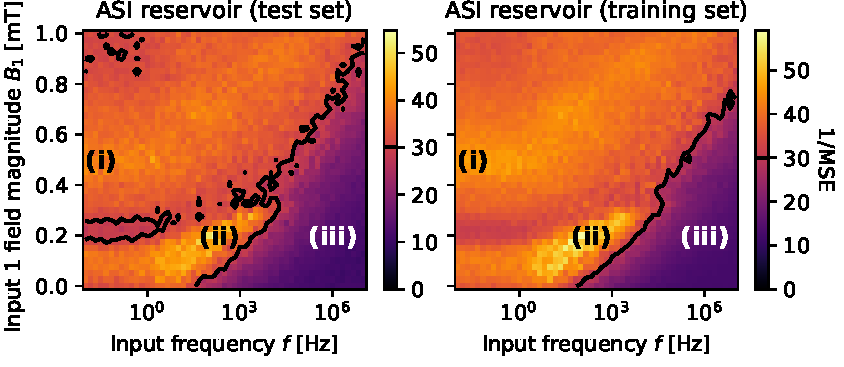
\includegraphics[width=\linewidth]{3_RC_OOP/Thermally active/Transformation/freq-magn/baseline/averaged.pdf}\\
	\vspace{-1em}
	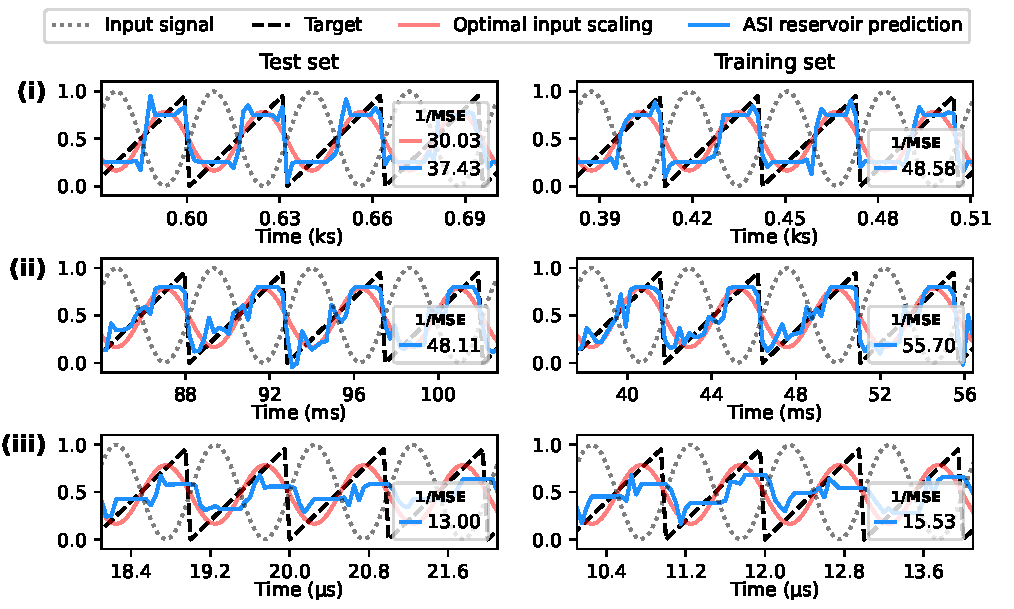
\includegraphics[width=\linewidth]{3_RC_OOP/Thermally active/Transformation/freq-magn/baseline/details.pdf}
	\vspace{-2.5em} % Looks more natural for this figure
}{
	\label{fig:3:Transformation_freq-magn_baseline}
	Monte Carlo simulations of a sine-to-sawtooth signal transformation performed by a thermally active $11 \times 11$ OOP square-lattice ASI reservoir.
	The top panel shows the inverse mean squared error $1/\MSE$ as a function of the input magnetic field frequency $f$ and amplitude $B_1$, with constant $B_0 = \SI{-0.35}{\milli\tesla}$, averaged over 5 runs with random $\sigma(\EEA)=\SI{5}{\percent}$ defects.
	Higher (lower) values in yellow (purple) indicate better (worse) performance.
	The black contours correspond to $1/\MSE \sim 30$, encompassing regions where the reservoir performs better than the linear transformation of the original input signal.
	In the top figure, several points are indicated with Roman numerals, corresponding to the panels at the bottom of the figure which show a temporal view of the transformation.
	There, the input sine-wave signal (black dotted curve) and target sawtooth signal (black dashed line) are shown, alongside the prediction with and without the reservoir (blue and red curve, respectively) for different input frequencies and field magnitudes.
}
\vspace{-1em}

To better capture the slope of the sawtooth, a faster input frequency is required.
It turns out that, for this baseline system, a rather broad range of well-performing input frequencies exists between $f \approx \SIrange{10}{e3}{\hertz}$, in combination with a maximum field magnitude $B_1 \approx \SI{0.2}{\milli\tesla}$, as indicated by the symbol \textsf{(ii)}.
Such a broad range of usable frequencies was to be expected considering the logarithmic nature of the relaxation dynamics.
With such input, the waveform resembles a sawtooth much better than for low-frequency input.
Still, the waveform is quite noisy due to the stochastic nature of the reservoir.
While the bottom of the sawtooth is captured rather well, the top exhibits a plateau --- this coincides with the minimum of the input sine wave, meaning the system is given too much time to relax. \par
Increasing the frequency further has a negative impact on the transformation, as is the case for \textsf{(iii)}.
The system becomes increasingly unable to approach the $\mavg \approx 0$ state and can only respond to the input when it is sufficiently strong, as evidenced by the sloped $1/\MSE=30$ border that separates points \textsf{(ii)} and \textsf{(iii)} in the top panels of~\cref{fig:3:Transformation_freq-magn_baseline}.
Instead, while there is still some periodic structure visible in the waveform generated by reservoir \textsf{(iii)}, it is dominated by noise since only a few random magnets will switch in the limited available timeframe.

\subsubsection{Parameter dependencies}
\paragraph{Field magnitude range}
The minimal field magnitude $B_0$ for the baseline system in~\cref{fig:3:Transformation_freq-magn_baseline} was set to \SI{-0.35}{\milli\tesla}.
This was determined through a similar parameter sweep over $B_0$ and $B_1$, at a constant frequency $f=\SI{100}{\hertz}$ since this corresponds to the timescale at which this system reaches $\mavg \approx 0$ (according to panel 8 in~\cref{fig:3:OOP_relaxation}).
The results of this parameter sweep for the baseline system are presented in~\cref{fig:3:Transformation_magn-magnmin}: 
indeed, optimal performance is found around $B_0=\SI{-0.35}{\milli\tesla}$.

\vspace{-1em}
\sidefig[0.53]{3_RC_OOP/Thermally active/Transformation/magn-magnmin/averaged.pdf}{
	\label{fig:3:Transformation_magn-magnmin}
	Inverse mean squared error $1/\MSE$ of a sine-to-sawtooth signal transformation using a thermally active $11 \times 11$ OOP square-lattice ASI, as a function of the input magnetic field range $B_0 \rightarrow B_1$ at a constant input frequency $f=\SI{100}{\hertz}$.
	Averaged results are shown over 5 runs with random $\sigma(\EEA)=\SI{5}{\percent}$ defects.
	Higher (lower) values in yellow (purple) indicate better (worse) performance.
	The black contours correspond to $1/\MSE \sim 30$, encompassing regions where the reservoir performs better than the linear transformation of the original input signal.
}

A point symmetry is visible about the origin of~\cref{fig:3:Transformation_magn-magnmin}: $\MSE(B_0, B_1) = \MSE(-B_0, -B_1)$.
The reason for this is the planar symmetry of the ASI, whose operation remains identical when it is flipped upside down.
While the optimal input frequency often remains of a similar order of magnitude regardless of the transformation --- since the frequency is mostly dictated by the relaxation dynamics --- the optimal range of input field magnitudes is highly dependent on the desired transformation.
For example, performance is somewhat reduced along the $B_0 = -B_1$ diagonal for the sine-to-sawtooth transformation considered here because this choice of input puts the sharp drop of the sawtooth at the moment when the input field is zero.
Other transformations can behave very differently: this kind of $\MSE(B_0, B_1)$-map can be used to identify their optimal input field range at a given frequency.

\paragraph{Gradient}
The baseline system does not include a property gradient.
By making the magnets on one side of the system bigger than on the other side, the relaxation timescales can be spread out throughout the system, introducing more variation between the single-column readout nodes.
Quantitatively, in an ASI with a gradient $\Gamma$, the net OOP anisotropy $\EEA$ and magnetic moment $\mu$ on the right (left) side of the lattice are a factor $\Gamma$ higher (lower) than the average.
The varying magnetic moment $\mu$ also affects the NN MS coupling: the previously stated constant value of $\EMC = 2.5 \kBT$ now corresponds to the MS coupling between NN if their moment $\mu$ would be equal to the average magnetic moment $\llangle \mu \rrangle$ throughout the ASI.

\vspace{-1em}
\sidefigs[0.53]{3_RC_OOP/Thermally active/Transformation/grad-magn/freq1/averaged.pdf}{3_RC_OOP/Thermally active/Transformation/grad-magn/freq1/details.pdf}{
	\label{fig:3:Transformation_grad-magn_freq1}
	Impact of the \xref{property gradient} $\Gamma$ on the performance of a sine-to-sawtooth signal transformation by an $11 \times 11$ OOP square-lattice ASI reservoir.
	The top panel shows the inverse mean squared error $1/\MSE$ as a function of the gradient $\Gamma$ and amplitude $B_1$, with constant $B_0 = \SI{0}{\milli\tesla}$, averaged over 5 runs with random $\sigma(\EEA)=\SI{5}{\percent}$ defects.
	Higher (lower) values in yellow (purple) indicate better (worse) performance.
	The black contours correspond to $1/\MSE \sim 30$, encompassing regions where the reservoir performs better than the linear transformation of the original input signal.
	The panel at the bottom provides a temporal view of the transformation for a gradient $\Gamma = \SI{52}{\percent}$ and $B_1=\SI{0.45}{\milli\tesla}$, showing the input sine-wave signal (black dotted curve) and target sawtooth signal (black dashed line) alongside the prediction with and without the reservoir (blue and red curve, respectively).
}

The impact of such a gradient is illustrated in~\cref{fig:3:Transformation_grad-magn_freq1} as a function of the input magnitude $B_1$.
A low input frequency of $f=\SI{1}{\hertz}$, constant throughout the figure, to assess whether the introduction of a gradient can improve upon the square-wave signal that was generated for low-frequency input in~\cref{fig:3:Transformation_freq-magn_baseline}.
Indeed, with the optimal gradient for this particular system, $\Gamma \approx \SI{50}{\percent}$, the transformation no longer resembles a square wave despite the low frequency. \par
For even stronger gradients, the performance drops again, as the range of anisotropies $\EEA$ in the system becomes too wide for an input signal to effectively induce dynamics throughout the whole system.
It can also be noted that the range of suitable input magnitudes $B_1$ expands as the gradient becomes more severe.
The reason for this is that the range of coercive fields of individual magnets in the system gets wider due to the property gradient.
As a final note, the minimal input magnitude in this example was chosen as $B_0=\SI{0}{\milli\tesla}$ to illustrate that the value of $B_0$ is clearly identifiable in such heatmaps by a constant and very low value of $1/\MSE$ at $B_1=B_0$.

\paragraph{System size and readout resolution}
Increasing the number of magnets $N$ in the ASI reduces the relative impact of thermal noise, since each readout node then averages over more magnets.
The central limit theorem states that the standard deviation of a mean scales as $1/\sqrt{N}$, so the relaxation trajectories based on $\mavg$ will be more reproducible in larger systems.
Hence, increasing the size of the system is expected to enhance the transformation quality as the perceptron output then also becomes less noisy. \par
When each readout node represents the average magnetisation of one column, a square $L_x \times L_y$ ASI yields $p = L_x = L_y$ nodes ($\vc{r}(t) \in \mathbb{R}$).
However, as $p$ increases, the danger of overfitting increases as well~\cite{DeepRC_IonGating_Overfitting,lukovsevivcius2009reservoir}.
Overfitting is a general machine learning phenomenon that occurs when a model has too many trainable weights $\vc{w}$ for the limited data it has been given.
This causes the model to train on noise present in the data --- rather than on the general trend underlying that noisy data --- resulting in worse performance on the test set.
Since our thermally active OOP ASI reservoir is inherently noisy due to thermal fluctuations, overfitting is a possible concern.
Overfitting is the main reason why data is typically split into a training and test set, as the $\MSE$ on the training set may be too optimistic a measure for the reservoir performance. \par
The reservoir performance with such single-column readouts is shown in~\crefSubFigRef{fig:3:Transformation_size-magn}{a}, as measured by $1/\MSE$ on both the training and test sets as a function of $p=L_x=L_y$.
At small $p$, performance is similar on both the training and test sets.
However, as $p$ increases, the training performance eventually improves more rapidly than the test performance --- for instance, at $p=100$, the training set $1/\MSE$ is approximately 120, whereas the test set $1/MSE$ barely surpasses 75.
This is a clear indication of overfitting. \par
Overfitting can be avoided by limiting the amount of readout nodes, for example by averaging multiple columns together.
The performance with a total of $p=11$ readout columns is presented in~\crefSubFigRef{fig:3:Transformation_size-magn}{a} as a function of system size $L_x = L_y$ and the input magnitude $B_1$.
Contrary to the single-column readout, the performance is now equal between the training and test sets, reaching a maximum of $1/\MSE \approx 60$ for $L_x=L_y=30$ beyond which enlarging the system no longer significantly affects the performance.

\vspace{-1em}
\makeshiftfig{
	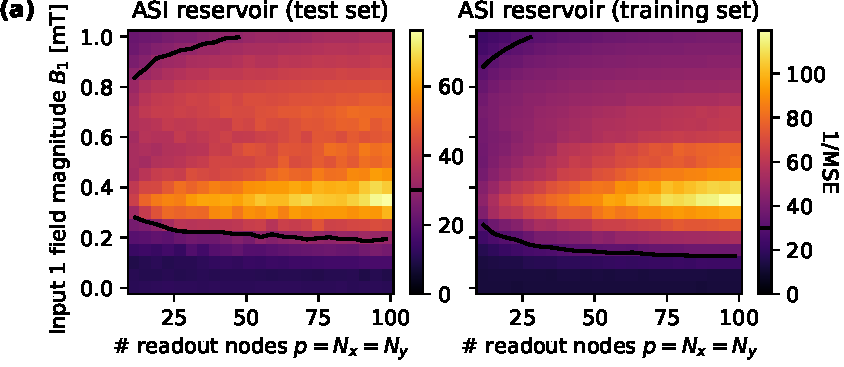
\includegraphics[width=\linewidth]{3_RC_OOP/Thermally active/Transformation/size-magn/resx==size/averaged.pdf}\\
	%\vspace{-1em}
	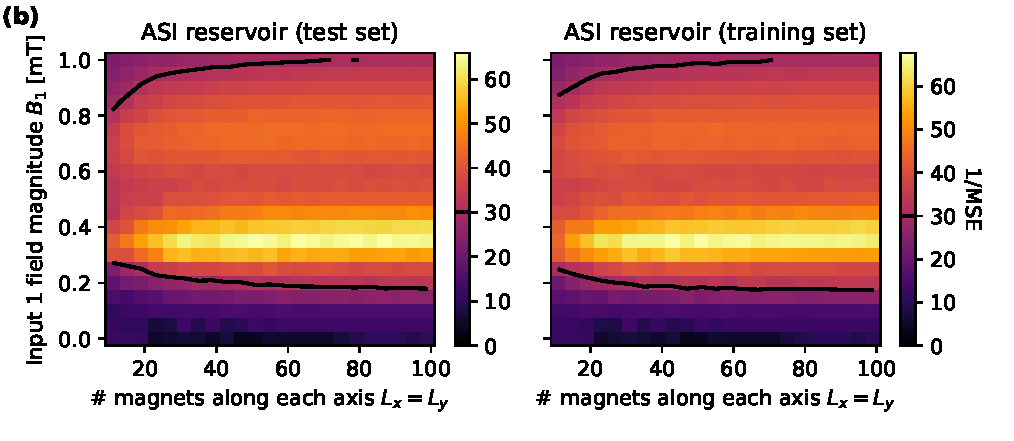
\includegraphics[width=\linewidth]{3_RC_OOP/Thermally active/Transformation/size-magn/resx=11/averaged.pdf}
	\vspace{-2.5em} % Looks more natural for this figure
}{
	\label{fig:3:Transformation_size-magn}
	Impact of system size on a sine-to-sawtooth signal transformation by an OOP ASI reservoir as measured by the inverse mean squared error $1/\MSE$ as a function of the input magnetic field magnitude $B_1$, averaged over 5 runs with random $\sigma(\EEA)=\SI{5}{\percent}$ defects.
	The input frequency and minimal magnitude were kept constant at $f=\SI{800}{\hertz}$ and $B_0=\SI{0}{\milli\tesla}$, respectively.
	Higher (lower) values in yellow (purple) indicate better (worse) performance.
	The black contours correspond to $1/\MSE \sim 30$, encompassing regions where the reservoir performs better than the linear transformation of the original input signal.
	In panel \textbf{(a)}, each column of the ASI constitutes an individual readout node, while in panel \textbf{(b)} the number of readout nodes was kept constant at 11 by averaging multiple columns together.
	The left (right) panels show performance on the test (training) set, to identify overfitting.
}
\vspace{-1em}

\paragraph{Double-frequency transformation}
For an appropriate set of system parameters --- with the input being applied at the right frequency and strength --- other transformations than the sine-to-sawtooth transformation can be targeted without changing the system.
Only the weights $\vc{w}$ of the perceptron have to be adjusted.
For example,~\cref{fig:3:Transformation_freq-magn_SINESQ} shows results for a double-frequency sine wave as target function. \par
For this transformation, the best fit attainable with a linear scaling of the input signal is simply a constant, as represented by the red line in the waveform at the bottom of~\cref{fig:3:Transformation_freq-magn_SINESQ}.

\sidefigs[0.53]{3_RC_OOP/Thermally active/Transformation/freq-magn/target_SINESQ/Sweep20231023131601.pdf}{3_RC_OOP/Thermally active/Transformation/freq-magn/target_SINESQ/details.pdf}{
	\label{fig:3:Transformation_freq-magn_SINESQ}
	Transformation of a sine wave input signal into a double-period sine wave by an $11 \times 11$ OOP square-lattice ASI reservoir.
	The top panel shows the inverse mean squared error $1/\MSE$ as a function of the input frequency and amplitude $B_1$, with constant $B_0 = \SI{0}{\milli\tesla}$.
	Higher (lower) values in yellow (purple) indicate better (worse) performance.
	The black contours correspond to $1/\MSE \sim 8$, encompassing regions where the reservoir performs better than the linear transformation of the original input signal.
	The panel at the bottom provides a temporal view of the transformation for $f=\SI{0.5}{\hertz}$ and $B_1=\SI{0.25}{\milli\tesla}$, showing the input sine-wave signal (black dotted curve) and target double-frequency sine (black dashed line) alongside the prediction with and without the reservoir (blue and red curve, respectively).
}

For the ASI to accurately produce a double-frequency sine, the input frequency must not be too high, as otherwise the system dynamics can not keep up to accurately produce a sine of double that period.
Therefore, the quality of the double-period sine quickly deteriorates above the critical frequency $f_c \approx \SI{10}{\hertz}$.
It is no coincidence that this value is similar to the timescale at which $\mavg \approx 0$ in panel 8 of~\cref{fig:3:OOP_relaxation}, which shows the relaxation in the absence of external stimuli for this system.
The same cut-off at $f_c$ is observed when the target is a square wave, though this is not displayed in a figure as a sine-to-square transformation is not otherwise noteworthy.

\subsection{Signal prediction task: chaotic Mackey-Glass oscillator}
A special kind of ``transformation'' is a signal prediction, where the target function $y(t) = s(t + \Delta t)$ is essentially the input signal offset through time.
Such a prediction task can make use of the fading memory property of a reservoir to better infer the future evolution of the signal, while it benefits less from a reservoir's non-linearity~\cite{TaskAdaptivePRC}.
The particular signal we will be attempting to predict with the thermally active OOP ASI is the chaotic Mackey-Glass oscillator $\mathrm{MG}(t)$~\cite{MackeyGlass}, as this is a popular benchmark in literature~\cite{RotatingNeuronsRC,AdaptiveProgrammableRC,TaskAdaptivePRC,Moon_2021,JaegerHaasWireless,ArchitecturalMarkovianESN}.
It can not be written in closed form; instead, it is implicitly defined by the delay-differential equation
\begin{equation}
	\label{eq:3:MG}
	\frac{d\mathrm{MG}(t)}{dt} = \frac{\beta \mathrm{MG}(t - \tau)}{1 + \mathrm{MG}(t - \tau)^n} - \gamma \mathrm{MG}(t) \mathrm{,}
\end{equation}
which was discretised by a time step $\tau/1000$ following~\ccite[Appendix A]{MeasuringStrangenessAttractors}.
Typical values for the parameters $\beta=0.2, \gamma=0.1$ and $n=10$ were used.
For $\tau \gtrsim 16.8$, this system is chaotic~\cite{jaeger2001echo}: $\tau=23$ was used here to get sufficiently chaotic behaviour, though $\tau=17$ is a more common choice.
To extinguish transients after releasing the oscillator from its initial state (set to $\mathrm{MG}(t \leq 0) = 0.5$), a first timeframe of $t \leq 25\tau$ is discarded.
Meanwhile, the extrema attained during this initial timeframe were recorded to allow a scaling of subsequent input to the appropriate field range between $B_0$ and $B_1$. \par
While the Mackey-Glass oscillator is not strictly periodic, its delay parameter $\tau$ still provides a characteristic timeframe for its oscillations.
Therefore, the specific transformation attempted here is written as
\begin{equation}
	s(t) = \mathrm{MG}(ft\tau) \mapsto y(t) = \mathrm{MG}((ft + h)\tau) \mathrm{,}
\end{equation}
where $f$ fulfils the role of a ``frequency'' to synchronise the Mackey-Glass oscillator with the reservoir's relaxation dynamics despite the non-periodic nature of the signal.
This also provides the definition of the ``offset'' $h$, i.e. a dimensionless measure for how far ahead the reservoir must predict, which has a large impact on the quality of the prediction. \\\par

The previous discussion regarding the signal transformation task demonstrated that many system parameters --- including the input frequency $f$, the input magnitudes $B_0$ and $B_1$, the size $L_x \times L_y$ of the ASI, the \xref{property gradient} $\Gamma$, the number of readout nodes $p$ \dots --- affect the transformation quality.
Since the absolute values of $f$, $B_0$ and $B_1$ provide limited additional insight, we will henceforth use Bayesian optimisation~\cite{BayesOpt_Mockus1975} over the $f \times B_0 \times B_1$-space to identify the optimal input characteristics for a given ASI. \par % This was not done for the figures relating to the signal transformation task, as it would be prohibitively expensive to compute the optimal system parameters for each pixel in those figures.
This allows us to concentrate on the most critical variable for a prediction task: the offset $h$, whose impact is illustrated in~\crefSubFigRef{fig:3:Prediction_MG}{a} for three particular systems with a different size and \xref{property gradient}.
For the systems with a gradient, $\Gamma$ was also optimised during the Bayesian optimisation procedure, which typically yields $\Gamma \approx \SIrange{25}{30}{\percent}$, though less severe gradients also perform decently. \par

Most strikingly, as a function of the offset $h$, the optimum MSE\footnote{
	\crefSubFigRef{fig:3:Prediction_MG}{a} uses $\MSE$ rather than $1/\MSE$, as $1/\MSE$ for $h=0$ is much larger than for other $h > 0$.
	Furthermore, it is most common in literature to use $\MSE$ when reported as a function of the offset $h$.
} exhibits both a maximum and a minimum.
The resulting wave-like appearance of $\MSE(h)$, typical for this kind of input signal~\cite{AdaptiveProgrammableRC,ForecastingNeuralODE}, originates from the definition of $\mathrm{MG}(t)$ as a delay-differential equation~\eqref{eq:3:MG}.
The characteristic delay $\tau$ makes it easier to predict $\mathrm{MG}(t + \tau)$ --- a delay $\tau$ corresponds to $h=1$, which closely aligns with the observed minimum of $\MSE(h)$.
For larger offsets $h$, more such minima will appear close to $h \in \mathbb{N}$, though they become increasingly less pronounced because the oscillator is not strictly periodic over $\tau$.
The height of the first maximum can be used as a performance indicator to compare different reservoirs. \par
The performance at $h=0$ presents the limit of what the thermally active ASI reservoir can achieve, due to the stochastic nature of the relaxation process it employs.
Unsurprisingly, this limit improves by adding a gradient and increasing the system size.

\vspace{-1em}
\xfig{3_RC_OOP/Thermally active/Prediction/MG.pdf}{
	\label{fig:3:Prediction_MG}
	Performance of a thermally active OOP square-lattice ASI on a prediction task for the Mackey-Glass oscillator, for ASI of different size and gradient $\Gamma$.
	The number of readout nodes is fixed at $p=11$ for the $11 \times 11$ systems and $p=10$ for the $20 \times 20$ ASI.
	\textbf{(a)} Mean-squared error as a function of the offset $h$, for the reservoir prediction (blue) and a linear transformation of the original input signal (red).
	The ultimate performance limit of each reservoir, i.e. $\MSE(h=0)$, is indicated by the horizontal grey dotted line.
	\textbf{(b)} Comparison of waveforms generated by an $11 \times 11$ ASI without a gradient (left) and a $20 \times 20$ ASI with a gradient $\Gamma = \SI{10}{\percent}$ (right), both for an offset $h=1.4$.
}
\vspace{-0.5em}

The $11 \times 11$ ASI reservoir without gradient (blue) only outperforms a linear scaling of the input (red) for $h > 0.4$.
Including a gradient and enlarging the system improves the $\MSE$, though the gradient appears more impactful than a subsequent enlargement.
More importantly than the $\MSE$, the resulting waveform is also of better quality, as~\crefSubFigRef{fig:3:Prediction_MG}{b} shows for $h=1.4$.
The smaller ASI without gradient struggles to reproduce the peaks of the desired waveform, as it only responds in a narrow field range.
On the other hand, the larger ASI with an appreciable gradient $\Gamma \approx \SI{25}{\percent}$ contains magnets of various coercive fields, enabling it to capture both the peaks (valleys) since these are likely to coincide with low (high) input fields.
%Besides the peaks and valleys, also the relatively constant $y(t)$ from $t=\SIrange{0.732}{0.736}{\second}$ is captured decently by the reservoir.

\subsection{Comparison with other reservoirs}
While a signal transformation and prediction performed using this kind of reservoir is not perfect, it is of comparable quality to several other magnetic reservoirs.
Generally speaking, the thermally active OOP ASI presented here achieves $\MSE \gtrsim 0.015$, both for signal transformation and a Mackey-Glass prediction.
A system of magnetic nanorings has been demonstrated to yield a very similar $\MSE \approx 0.014$ on a sine-to-sawtooth transformation~\cite{Vidamour2023}.
Comparable results have been obtained with an artificial spin-vortex ice reservoir, which achieves $\MSE \approx 0.019$ for a sine-to-sawtooth transformation and $\MSE \approx 0.01$ for a Mackey-Glass prediction at $k \approx 1.4$~\cite{gartside2022reconfigurable}.
Combining multiple in-plane square and pinwheel ASI reservoirs in series has resulted in $\MSE \approx 0.011$ for Mackey-Glass with $k \approx 0.8$ and $\MSE \approx 0.01$ on a sine-to-sawtooth transformation~\cite{AdaptiveProgrammableRC}. \par
Reconfigurable reservoirs are typically more performant as they can adapt to the task at hand.
One example of these is a skyrmion/conical reservoir~\cite{TaskAdaptivePRC}, which obtains a better sine-to-sawtooth transformation ($\MSE \approx \SIrange{e-4}{3e-7}{}$) and Mackey-Glass signal prediction ($\MSE \approx 0.0037$), though only at very low temperature $T = \SI{4}{\kelvin}$.
Above room temperature, $\MSE \approx 0.018$ was reported for an offset $k \approx 0.25$, again similar to the thermally active OOP ASI. \par

Other types of reservoirs exists beside magnetic reservoirs.
For example, nanowire networks~\cite{RC_NNN} exhibit more complex dynamics, allowing them to achieve a better signal transformation.
A carbon nanotube reservoir, for example, has been used to get $\MSE \approx 0.008$ on a sine-to-sawtooth transformation~\cite{CarbonNanotubeRC}.
Others~\cite{NanoarchitectonicAtomicSwitch,FewMoleculeReservoir} achieve similar performance.
Chemical dynamics can also be utilised as a reservoir: , for which $\MSE \approx 0.002$ has been demonstrated in a sine-to-sawtooth task~\cite{ElectrochemicalPRC}. % that's for Polyoxometalate, $\MSE \approx 0.04$ for water
A mathematical echo state network has reportedly achieved $\MSE \approx 0.006$ for a very far future prediction of $k \approx 5$~\cite{Moon_2021}. % They gets NRMSE of 0.045 for their single-reservoir ESN, which corresponds to MSE 0.002, but their definition divides the normal MSE by the average square deviation, which is never more than 0.25. So the correspondence is quite vague.

\subsection{Conclusion}
By harnessing the spontaneous relaxation dynamics of thermally active OOP ASI, coupled with their gradual response to an external stimulus, these kinds of systems can be used as a reservoir.
Including a property gradient and enlarging the ASI both provide a boost to the computational capability.
However, the working principle adopted here inevitably suffers from thermal noise, which imposes a limit to the achievable performance of these systems.
Nonetheless, thermally active OOP ASI performs comparably to many other single reservoirs on signal transformation and prediction tasks.
A major advantage of thermally active ASI is that they can respond to a wide range of input frequencies --- spanning two orders of magnitude or more --- owing to the logarithmic nature of the relaxation dynamics.

% MSE is not an ideal parameter, should use something that accounts more for the general shape, because plateaus can have equal weight as noise, while they are visually quite different.

\newpage
\section{Reservoir computing in non-volatile out-of-plane ASI}
We now turn our attention to non-volatile ASI, to show that an ASI need not be thermally active to use it for reservoir computing.
When the energy barrier $\EEA$ of a magnet is significantly higher than the thermal energy $\kBT$, the N\'eel-Arrhenius switching law implies that it will remain stable over any reasonable timescale in the absence of external perturbations.
For example, a magnet with $\EEA > 40 \kBT$ will most likely remain stable for multiple years.
Therefore, non-volatile ASI is easier to construct than thermally active ASI, as great control over the perpendicular anisotropy is not required --- the anisotropy just has to be sufficiently large.
Throughout this section, we will develop, examine and discuss a ``clocked'' input protocol for non-volatile ASI that exhibits promising memory capacity.

\paragraph{Magnetostatic interaction}
Note that a ``non-volatile'' system is not the same as a non-interacting system.
While a low magnetostatic coupling $\EMC \ll \EEA$ results in a frozen system, a sufficiently high coupling will still induce spontaneous ordering, albeit only locally as the high anisotropy renders domain walls immobile.
Recall in this regard the five regions previously outlined in~\cref{fig:3:OOP_relaxation_continuous}.
Because of the high anisotropy $\EEA$, the superparamagnetic region~$\mathrm{V}$ and perfectly ordered region~$\mathrm{IV}$ are not relevant.
Instead, non-volatile ASI only exhibit two regimes: one where the magnetostatic coupling is sufficiently strong to overcome the energy barrier $\EEA$, and another where it is not.
These respectively correspond to region~$\mathrm{III}$~and~$\mathrm{I}$, while region~$\mathrm{II}$ is simply a smooth transition between these two regimes.
If, however, the RC input method does not cause significant local deviations from the ground state --- by for instance using domain wall motion for computation --- then these two regimes are equivalent from an RC perspective. \par

% Nomenclature: thermally active ASI has low energy barriers that allow the domain walls to move by thermal fluctuations, as all interactions are on the order of several $\kBT$. Spontaneously relaxing ASI just has a sufficiently strong MS interaction for domains to form, but domain walls will remain fixed in place when $\EMC$ or $\EEA$ is high. \par
% Achieving computation in a frozen system (i.e., region~$\mathrm{I}$) requires careful tuning of the strength of the input stimulus and the $\EMC/\EEA$ balance.

While the thermally active ASI typically had a MS coupling $\EMC \lesssim 10\kBT$, as was determined from the MFM images in~\cref{fig:3:MFM_grid}, such low coupling will be insufficient in non-volatile ASI.
For deterministic switching, both the anisotropy $\EEA$ and magnetostatic coupling $\EMC$ must be sufficiently high, say $\gg 40 \kBT$.
Increasing the magnetostatic coupling beyond $10\kBT$ should not present a significant practical issue, as the inclusion of a separate ferromagnetic layer above the magnets can significantly increase the MS coupling by focusing the stray fields onto nearby magnets~\cite[Supp. 10]{KUR-24}.

\paragraph{Uniform external field}
While it was possible to achieve decent signal transformation in thermally active OOP ASI by using a uniform external field, this approach is no longer viable in non-volatile ASI.
They lack the intrinsic relaxation dynamics that RC in thermally active ASI relied on, so a fundamentally different input method will be required.
In a non-volatile system, the temporal dimension is irrelevant, as a magnet will either switch within a reasonable timeframe or it will not.
Therefore, we must instead make use of the spatial dimensions of an ASI to perform RC.
Rather than pulling the system away from equilibrium and expecting it to evolve back to the ground state all by itself, we can instead use the domain structure for computation.

\subsection{Two-step input protocol: clocking}
To achieve control over the domains, we can take inspiration from the ``clocking'' protocol proposed by Jensen~\textit{et al.}~\cite{clocking-protocol}, which can move domain wall boundaries in IP pinwheel ASI in discrete steps.
While our square-lattice OOP ASI is very different from the pinwheel lattice, both exhibit domains, though these are superferromagnetic in pinwheel ASI rather than anti-ferromagnetic.
As such, some key concepts can be carried over, but the specific realisation of input and readout will have to be altered significantly to make such a clocking protocol work well for OOP ASI. \par
To achieve clocking, Jensen~\textit{et al.}~\cite{clocking-protocol} applied an external magnetic field in a well-chosen direction to selectively affect one of the two pinwheel sublattices at a time, and then changed the field direction to affect the other sublattice.
By carefully tuning the field magnitude, only the magnets at the boundary of a domain --- or at the edge of the ASI --- will switch.
This is possible because those magnets have a lower effective energy barrier $\EBeff$ than magnets in the bulk of a domain.
Such a two-step clocking protocol therefore allows domain wall boundaries to advance one step at a time, while avoiding saturated magnetic states that would result from a stronger input. \par
The key takeaway from this concept is that two key factors are necessary if one wants to achieve controlled domain wall movement in any ASI~\cite{MAES-24}.
\begin{itemize}
	\item The input method must lift the degeneracy between the ground states --- in pinwheel ASI, a global in-plane field readily distinguishes between the four types of superferromagnetic domains.
	\item At least two independently addressable sublattices should exist to prevent avalanches --- in pinwheel ASI, two sublattices exist whose magnets are perpendicular to each other, enabling selective manipulation via in-plane fields.
\end{itemize}
Let us now consider the specifics how this can be achieved in a square-lattice OOP system.
This system is quite different from the IP pinwheel lattice used by Jensen~\textit{et al.}~\cite{clocking-protocol} and will therefore require a different input method than just applying uniform fields at well-chosen angles.

\paragraph{Distinguishing between the degenerate ground states}
\subparagraph{Uniform field}
A uniform external field, as was successfully used in thermally active ASI, does not fulfil the first requirement.
It can not distinguish between the two checkerboard ground states, as it affects domains of both types equally and can therefore not be used in a clocking protocol.
In fact, a uniform field is not suited for RC in any non-volatile ASI that does not exhibit superferromagnetic domains, as it simply causes the magnetisation of low-$\EBeff$ magnets to align with the external field.
Any subsequent input cycle of opposite sign would either be too weak to have any additional effect, or be strong enough for the previously switched magnets to switch back, after which the same unremarkable process can repeat.
Regardless, a uniform field will not obtain the much coveted fading memory, precluding its use for RC in this system.
Hence, for an input protocol to induce desirable dynamics in non-volatile ASI, it must be specifically tailored to the lattice geometry.

\subparagraph{AFM input}
In the specific case of square-lattice OOP ASI, the two degenerate domain types can be separately addressed by applying an AFM ``checkerboard'' field --- a spatially alternating up/down external field where each magnet experiences an oppositely oriented field compared to its nearest neighbours\footnote{
	A practical realisation of such an AFM stimulus could be based on SOT induced by diagonal current lines, such that successive diagonals carry oppositely oriented currents, resulting in the required checkerboard pattern.
	Care must be taken, however, that this input is compatible with the AHE readout, which requires a full conducting layer rather than individual diagonal current lines.
	Since we focus on the theoretical potential of OOP ASI for RC, any additional practical considerations are beyond the scope of this thesis.
	% See rudimentary figure 20250403 for global vs clocked AFM input concept.
	% For global AFM input, the concept is to use a "snake" diagonal current line to get the alternating +/- checkerboard ordering, but the AHE underlayer is problematic as it enables short-circuiting such that the current does not follow the snake.
	% For clocked AFM input, the concept is to use "diagonally interlaced fingers" and only run current through half of them to get the clocking. This should be mostly compatible with the AHE, though uneven current distribution may be a concern.
}.
This alternating field temporarily lifts the degeneracy between the two domain types while the input is applied, hence promoting domains of one type at the expense of the other.
Information can then be encoded into the system by mapping a positive input value to one domain type, while a negative input corresponds to the other.

\subparagraph{AFM readout}
The readout method must be able to pick up on the changes induced by the input for there to be a meaningful input-output relation to perform RC with.
In our case, using the domain types for computation requires a readout method that can distinguish between the ground states.
This precludes the usage of a local $\mavg$ readout, as used for the thermally active system, nor can the order parameters $\qNN$ be used.
Instead, the domain type of each magnet will henceforth be used as the readout quantity, by mapping the two equivalent domain types to the values $\pm 1$.
Recall that it is theoretically possible to determine the state of all magnets in a small ASI from AHE measurements~\cite[Supp. 7]{KUR-24}.
Hence, such an AFM readout is practically achievable since it only requires a multiplication of the state of each magnet by $\pm 1$, depending on their location in the ASI. \par
To turn these individual magnetic states into a robust output vector, we will once again use averaging to avoid overfitting.
Since the $x$- and $y$-axes are equivalent, this is done via ``squinting'' --- effectively dividing the ASI into a coarser square lattice and averaging the states of $k \times k$ magnets for each readout value.
Hence, absolute values $<1$ indicate the presence of a domain boundary and it is even possible to distinguish between straight domain walls, corners and other features based on these averaged readout values.
Since there are $\approx N/k^2$ readout values, overfitting can be avoided by choosing $k$ sufficiently large.
Typically, we use rather small ASI just like we did for thermally active ASI, so $k=2$ is often a good choice for systems up to $20 \times 20$ magnets.

\paragraph{Avalanches and saturation}
The previously discussed AFM input method, which applies a spatially alternating up/down field, is insufficient to achieve controlled domain wall movement.
Because it applies a global stimulus, it easily triggers avalanches of switching magnets, rather than stepwise domain wall motion.
This occurs because most domain wall magnets all experience a similar effective energy barrier $\EBeff$, regardless of their location.
Hence, when the input is strong enough to move a domain wall by one lattice unit, the local environment at this new location is unlikely to be sufficiently different to impede further motion.
As a result, within a single input cycle, domain walls continue moving until they either annihilate, reach the system's edge, or encounter an insurmountable defect. \par

% In this regard, the AFM input method is not fundamentally different from the uniform input strategy we previously dismissed. Both simply provide each magnet with a preferential orientation, with only high-anisotropy magnets refusing to switch. Given this similarity, one might be inclined to consider them mathematically equivalent when paired with their respective readout methods. However, while both methods ultimately lead to saturation and are therefore unsuitable for RC, they differ in how they affect the microstate of the system when the magnetostatic interaction is appreciable. \par Compared to the AFM input method, a uniform field must be far stronger to have any effect, as it has to switch all magnets to the highest-energy state where all magnets have the same magnetisation direction. While the AFM input method also just pulls magnets in a certain direction, it differs in that it pulls the ASI to one of the ground states. This allows it to achieve saturation already with a far weaker input, since it only needs to affect domain wall magnets which have just $\leq 3$ oppositely magnetized NN and are therefore stable with $\EBeff \propto \EEA + 2\EMC$, as compared to $\EEA + 4\EMC$ for bulk magnets. It is therefore far easier to propagate a domain wall through the system to switch the ASI to the opposite ground state, as compared to pulling the system away from this near-equilibrium state to a uniform state. \par Hence, the effect of both global input methods on the ASI is fundamentally different, even though they both achieve saturation near-instantaneously which precludes their usage for RC.
% Summary of the previous comment: Both the AFM input method and the uniform input impose a preferred magnetisation direction, leading to saturation and making them unsuitable for RC. However, they differ in how they interact with the system when magnetostatic interactions are significant. A uniform input requires a much stronger field to overcome the stability of bulk magnets, which have four anti-parallel NN. In contrast, the AFM input naturally drives the system toward one of its ground states and requires a weaker stimulus, as it primarily affects domain wall magnets which have fewer oppositely magnetised NN and are therefore easier to switch.

The fact that the AFM input can selectively influence domain walls is crucial, as it enables us to avoid saturation by introducing one last change to this input strategy.

\paragraph{Avoiding avalanches with a clocking protocol}
Saturation can be avoided by instead applying two sub-steps for each applied input value. As illustrated in~\cref{fig:3:Clocking_protocol}, the magnets are divided into two groups, akin to the black and white squares on a checkerboard.
In the first sub-step, the AFM stimulus is only applied to the first group, while the second sub-step only addresses the second group of magnets.
The strength and/or sign of the stimulus is determined by the input value.
We refer to this method as the \idx{two-step AFM clocking protocol}.
This way, since only half of the magnets are stimulated simultaneously, the other half is prevented from switching at the same time --- provided their anisotropy $\EEA$ is sufficiently high compared to the NN MS coupling $\EMC$.
The avalanches that plagued the global input strategies are thereby avoided. \par
For this to result in controlled domain wall motion, the strength of the input is of great importance.
If it is too weak, the magnets will not respond.
If the input is too strong, though, all magnets will follow the applied field and a global ground state will be reached within a single input cycle nonetheless.
However, a range of input strengths exists where only domain wall magnets respond to the input, since any domain wall magnet is less stable than a magnet in the bulk of a domain\footnote{
	Domain wall magnets, with 3 oppositely and 1 parallelly magnetised NN, experience $\EBeff = \EEA + \EMC$. Bulk domain magnets have 4 oppositely magnetised NN, and are therefore more stable with $\EBeff = \EEA + 2\EMC$.
}.
%This is no different from the global AFM input method, but that method had no way of stopping the domain wall movement after it had begun.
Hence, by combining an appropriate choice of input strength with the two-step protocol that prevents half of the magnets from switching, it is possible to move domain walls by only a few lattice sites at once. % by deterministically switching only domain wall magnets towards the applied field.

\xfig{3_RC_OOP/Nonvolatile/Clocking_protocol.pdf}{
	\label{fig:3:Clocking_protocol}
	 Illustration of the \xref{two-step AFM clocking protocol} for controlled domain wall movement in ASI.
	 The symbols $\bigodot$ and $\bigotimes$ respectively indicate that the external stimulus is such, that the magnet at that location would prefer an `up' or `down' magnetisation.
	 This example shows a $5 \times 5$ ASI, but the concept is analogous for other lattice sizes.
	 Each input cycle consists of two sub-steps that each affect a different set of magnets, arranged in a checkerboard pattern: only half of the magnets are stimulated at once.
	 Input cycle $A$ (associated with bit 0) and input cycle $B$ (bit 1) apply opposite stimuli.
}

To use this clocking protocol for RC, input values must be mapped to a certain magnitude of the input stimulus.
Since we intend to use of the stepwise growth (or shrinking) of domains over only one lattice unit at a time, it is most convenient to apply this two-step input protocol to binary input data.
Therefore, two cycles $A$ and $B$ are defined, associated with input bits `0' and `1', respectively. \par
Both cycles consist of two sub-steps, as illustrated in~\cref{fig:3:Clocking_protocol}.
Using the analogy of black and white squares on the checkerboard, the first sub-step of cycle $A$ causes magnets on black squares to prefer an `up' magnetisation, while the other magnets remain unaffected.
The stimulus is then removed, after which the second sub-step causes magnets on white squares to prefer a `down' magnetisation without affecting magnets on black squares.
These preferential magnetisation directions are illustrated in~\cref{fig:3:Clocking_protocol} by the symbols $\bigodot$ and $\bigotimes$.
Cycle $B$ is identical but promotes the opposite magnetisation direction for each magnet, in order to grow domains of the opposite type as compared to cycle $A$. \\\par
This clocking protocol, coupled with this definition of the input, readily provides basic memory in the system, as the previous few input bits become encoded in the size and location of the domains.
Since this clocking protocol relies on deterministic switching, the duration over which the sub-steps are applied is irrelevant\footnote{
	As time is irrelevant to non-volatile ASI, all simulations use a default duration of \qty{1}{\second} per input cycle.
}. \par
While this clocking protocol is likely not the only viable input method for non-volatile OOP ASI, we can at least say with certainty that simply applying a global uniform or AFM field would not yield any useful dynamics for RC.
In the remainder of this section, we will illustrate the behaviour of the clocking protocol and show that it yields desirable dynamics for RC.

\subsection{Illustrative examples}
To show that the \xref{two-step AFM clocking protocol} does indeed move domain walls step by step, independent of their orientation or precise location, we will now consider a few example systems.
This will illustrate that the growth of domains can be controlled as originally envisioned, while providing insight into the effect of system parameters on the domain wall motion.

\paragraph{Defect-free system}
First, for a clean illustration of the general behaviour of the clocking protocol, consider an example without any defects, i.e. $\sigma(\EEA) = \SI{0}{\percent}$.
The absence of defects results in a far more orderly domain wall motion than expected in a real system, where domain walls would be likely to remain pinned at high-anisotropy magnets.
The effect of subsequent clocking cycles on such a ``perfect'' system is shown in~\cref{fig:3:Clocking_clearly_EBstd0}.
The top half of this figure shows the magnetisation state of each magnet, while the bottom half shows the same states but instead visualises the two degenerate domain types as black and white.
% While diagonal domain walls stand out in the top panels as lines of the same colour, horizontal/vertical domain walls (e.g. in the centre of the ASI during the $B$ cycles) are harder to see.
Both are equivalent, but the domain representation is more insightful in this context since the entire appeal of this input method is controlled domain wall motion.
Therefore, only the domain representation will be shown in any subsequent figures.

\makeshiftfig{
	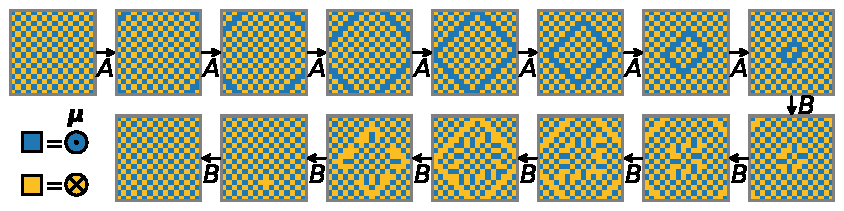
\includegraphics[width=\linewidth]{3_RC_OOP/Nonvolatile/Clocking_clearly_EBstd0_moments.pdf}
	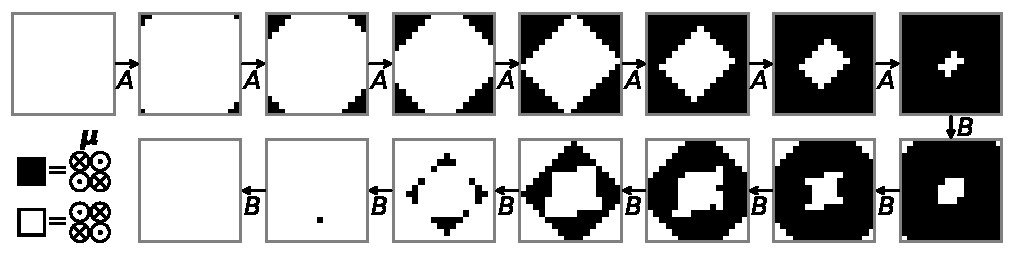
\includegraphics[width=\linewidth]{3_RC_OOP/Nonvolatile/Clocking_clearly_EBstd0_domains.pdf}
	\vspace{-1.5em} % Looks more natural for this figure
}{
	\label{fig:3:Clocking_clearly_EBstd0}
	Evolution of a $16 \times 16$ OOP square-lattice ASI when using the \xref{two-step AFM clocking protocol} (for seven cycles $A$ and seven opposite cycles $B$).
	The moment orientation (\textbf{top}) and domain type (\textbf{bottom}) of each magnet are shown after each cycle was applied.
	The finite size of magnets was accounted for with $D_\mathrm{NM} = \SI{170}{\nano\metre}$ and $S_\mathrm{ASI} = \SI{200}{\nano\metre}$.
	System parameters were chosen such that $\EMC = 40 \kBT$ and $\EEA = 200 \kBT$, with $\sigma(\EEA) = \SI{0}{\percent}$.
	All magnets are initially magnetised in one of the antiferromagnetic ground states (white).
	The magnetic field used in the clocking cycles has a magnitude $B_\mathrm{ext} = \qty{3.78}{\milli\tesla}$.
}

The figure clearly shows the stepwise growth of domains following the application of each individual clocking cycle.
While cycle $A$ promotes the domain type that is coloured black in the figure, cycle $B$ promotes the white-coloured domains.
These domains nucleate at the corners of the ASI, because those magnets only have two neighbours so their effective energy barrier $\EBeff$ is at least as low as that of a domain wall magnet.
During subsequent cycles, any existing domains of the type promoted by the applied cycle then grow at the expense of the opposite domain type. \par
A very important property of this input method is that cycle $A$ and $B$ are not each other's inverse, even though they only differ by the sign of their applied fields.
In the figure, this is reflected in the fact that the states visited by $B$-cycles were not previously visited by $A$-cycles.
Since some information from previous input cycles is often retained in this manner, this property provides the much coveted fading memory that is of great importance to RC. \par
Even though this system is non-volatile and defect-free, it can still exhibit some stochasticity.
One clear example of this is found in~\cref{fig:3:Clocking_clearly_EBstd0}: even though the three magnets at the bottom right switch during the first $A$-cycle, they do not switch during the first $B$-cycle.
The reason for this is the relatively low MS coupling $\EMC=40\kBT$, due to which the input strength must strike a delicate balance to avoid switching magnets that are not part of a domain wall.
These events can be suppressed by increasing the MS coupling, though a stronger input is then also required. \par % \\\par

Note also that, during the $B$-cycles in~\cref{fig:3:Clocking_clearly_EBstd0}, the central white-coloured domain does not re-grow with the same Petit-Beurre-shape\footnote{
	The ``Petit Beurre'' is a French biscuit decorated with serrated edges and four corners in the shape of ears, schematically resembling the central white-coloured domain that appears during the $A$-cycles of~\cref{fig:3:Clocking_clearly_EBstd0}.
} it previously had during the $A$-cycles.
Instead, it appears to preferably grow in such a way that it ends up with mostly horizontal and vertical edges, rather than diagonal ones.
This is part of the general phenomenon that, in the two-step AFM clocking protocol, domain growth preferentially occurs at the corners of a domain. \par
To more clearly illustrate this phenomenon,~\cref{fig:3:Clocking_massive_seeded} shows a far larger ASI which was initialised in one ground state, apart from one ``seed'' magnet at the centre which is of the opposite domain type as compared to all other magnets in the system.

\vspace{-1em}
\makeshiftfig{
	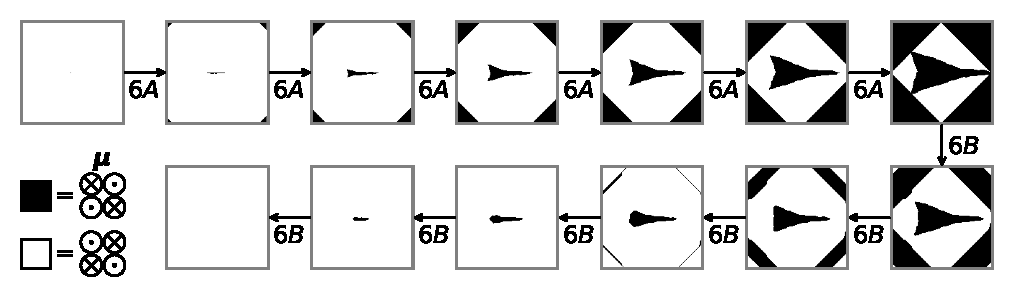
\includegraphics[width=\linewidth]{3_RC_OOP/Nonvolatile/Clocking_massive_seeded.pdf}
	\vspace{-1.5em} % Looks more natural for this figure
}{
	\label{fig:3:Clocking_massive_seeded}
	Evolution of a $141 \times 141$ OOP square-lattice ASI when using the \xref{two-step AFM clocking protocol} (for 36 cycles $A$ and 36 opposite cycles $B$).
	The domain type of each magnet is shown every six cycles.
	All magnets are initially magnetised in one of the antiferromagnetic ground states (white), apart from one magnet at the centre which started in the opposite state (black).
	The finite size of magnets was accounted for with $D_\mathrm{NM} = \SI{170}{\nano\metre}$ and $S_\mathrm{ASI} = \SI{200}{\nano\metre}$.
	System parameters were chosen to result in $\EMC = 40 \kBT$ and $\EEA = 200 \kBT$, with $\sigma(\EEA) = \SI{0}{\percent}$.
	The magnetic field used in the clocking cycles has a magnitude $B_\mathrm{ext} = \qty{3.78}{\milli\tesla}$.
}
\vspace{-1em}

During the first clocking cycle, one neighbour of the seed magnet will switch first, creating an asymmetry that causes the central domain to preferentially grow along that axis.
Magnets to the side of this elongated domain can also randomly switch, resulting in a gradual widening of the domain.
If this occurs at one of the domain's spearheads, whose tip is normally only 1 magnet thick, a small edge will be created that is 2 magnets long.
This is sufficient for the domain to fork into two diagonal directions since growth occurs preferentially at the corners of a domain.
This forking has occurred between the second and third panels of~\cref{fig:3:Clocking_massive_seeded}, but is a stochastic process: the right half of the domain in the figure did randomly fork. \par
Note also that, during the $B$-cycles in~\cref{fig:3:Clocking_massive_seeded}, white-coloured domains nucleate at the edges while the central white domain re-grows.
The white domains remain separated for about half as many $B$-cycles (18) as $A$-cycles were applied (36), at which time they reconnect and the rhombic black domain disappears.
Due to this imbalance, it is hard for domains to propagate far towards the centre when the input sequence contains equal amounts of each input bit.
Therefore, enhanced RC performance can be expected for systems with defects that allow domains to nucleate in the bulk of the system, or at least allow them to survive longer.

\paragraph{System with defects}
Any experimental realisation of OOP ASI will exhibit some degree of manufacturing defects, which are once again modelled by a normally distributed random anisotropy for each magnet in the ASI.
This results in more erratic states during successive steps of the clocking protocol as compared to the defect-free system from~\cref{fig:3:Clocking_clearly_EBstd0}.
However, contrary to the stochastic events mentioned before, the more erratic response caused by the disorder is reproducible and can therefore be used for computation. \par
The main reason for the more erratic response is that the difference between low- and high-barrier magnets in a system with defects can be substantial.
This often makes it impossible to find an input magnitude for which domain walls can propagate through any defect in the system without affecting magnets that are not part of domain walls.
Therefore, ``leaking'' can occur through low-barrier unstimulated magnets, which can spontaneously respond to the changing state of their neighbours even when they themselves are not stimulated~\cite{DisorderGroundStateASI}. % DisorderGroundStateASI says: "As expected, disorder allows dynamics to start inside the array at sites where ``loose'' spins with smaller switching fields are located."
This can be observed in~\cref{fig:3:Clocking_clearly_EBstd5} for an example with $\sigma(\EEA) = \SI{5}{\percent}$ and high MS coupling $\EMC = 200 \kBT$ compared to the anisotropy $\EEA = 100 \kBT$ to highlight leaking.

\makeshiftfig{
	%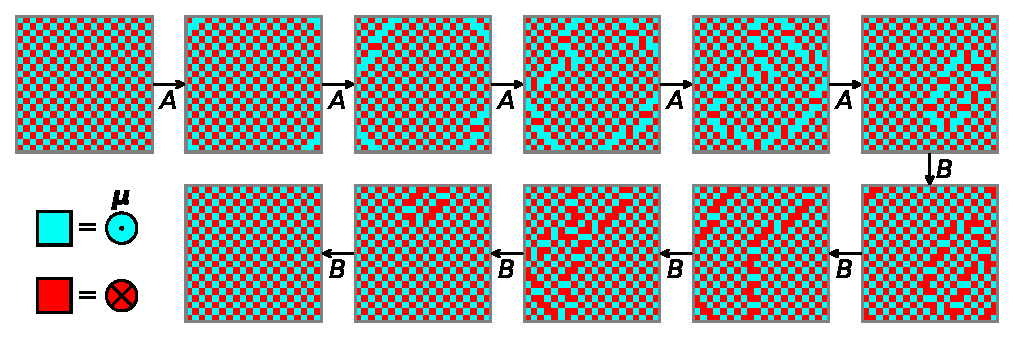
\includegraphics[width=\linewidth]{3_RC_OOP/Nonvolatile/Clocking_clearly_EBstd5_moments.pdf}
	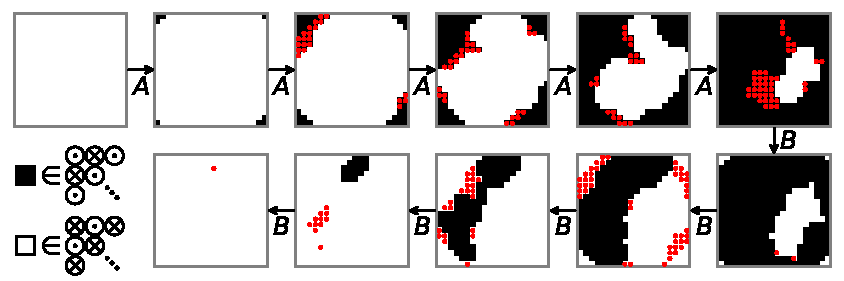
\includegraphics[width=\linewidth]{3_RC_OOP/Nonvolatile/Clocking_clearly_EBstd5_domains.pdf}
	\vspace{-1.5em} % Looks more natural for this figure
}{
	\label{fig:3:Clocking_clearly_EBstd5}
	Evolution of a $20 \times 20$ OOP square-lattice ASI when using the two-step AFM clocking protocol (for five cycles $A$ and five opposite cycles $B$).
	The domain type of each magnet is shown after each cycle.
	The finite size of magnets was accounted for with $D_\mathrm{NM} = \SI{170}{\nano\metre}$ and $S_\mathrm{ASI} = \SI{200}{\nano\metre}$.
	System parameters were chosen to result in $\EMC = 200 \kBT$ and $\EEA = 100 \kBT$, with $\sigma(\EEA) = \SI{5}{\percent}$.
	All magnets are initially magnetised in one of the antiferromagnetic ground states (white). The magnetic field used in the clocking cycles has a magnitude $B_\mathrm{ext} = \qty{5.5}{\milli\tesla}$.
}

Leaking can be mitigated by using a rather weak input, but this can make it impossible to switch some high-barrier magnets, rendering them frozen in their initial state.
This is to be avoided, as frozen magnets do not contribute to the fading memory of the system.
Alternatively, using a relatively strong input causes leaking but ensures that any magnet in the system can switch when required.
As long as domain walls do not move through too many unstimulated magnets per input step, leaking presents no issue.
It can even enhance RC performance, as it introduces asymmetry which is beneficial to the non-linearity of the system.
% Since leaking occurs due to low-barrier unstimulated magnets spontaneously switching in response to their neighbours, it is highly dependent on the magnetostatic interaction $\EMC$.

\paragraph{Energy balance}
As the ratio $\sigma(\EEA) \EEA / \EMC$ increases, so does the range of fields where low-anisotropy magnets can be switched in the bulk of a domain without significant leaking during stepwise domain wall propagation.
Such nucleation is beneficial for RC, in contrast to defect-free ASI where domain walls could only be injected at corners of the ASI.
%Fortunately from a fabrication perspective, systems with low $\EMC$ are typically easier to produce.
To illustrate the impact of $\EMC$,~\cref{fig:3:Clocking_clearly_EBstd5_EMC} compares a strongly-coupled system (a) with a weakly-coupled system (b). % a system with $\sigma(\EEA) \EEA / \EMC = 0.025$ (\crefSubFigRef{fig:3:Clocking_clearly_EBstd5_EMC}{a}) against one with $\sigma(\EEA) \EEA / \EMC = 0.25$ (\crefSubFigRef{fig:3:Clocking_clearly_EBstd5_EMC}{b}).
Indeed, nucleation occurs in the bulk of the weakly-coupled system because the disorder $\sigma(\EEA)\EEA=10\kBT$ is significant compared to $\EMC = 40 \kBT$, which also leads to far more irregular domain wall motion that encourages interactions between domain walls.

\vspace{-1em}
\makeshiftfig{
	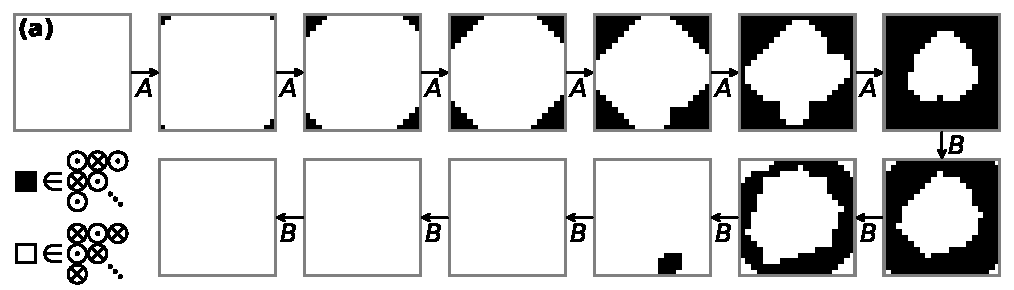
\includegraphics[width=\linewidth]{3_RC_OOP/Nonvolatile/Clocking_clearly_EBstd5_highEMC.pdf}\\
	\vspace{0.5em}
	\hrule
	\vspace{0.5em}
	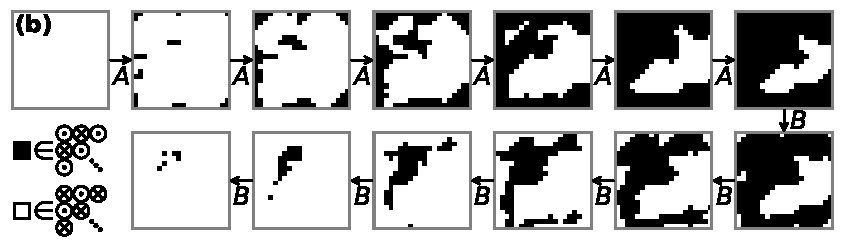
\includegraphics[width=\linewidth]{3_RC_OOP/Nonvolatile/Clocking_clearly_EBstd5_lowEMC.pdf}
	\vspace{-1.5em} % Looks more natural for this figure
}{
	\label{fig:3:Clocking_clearly_EBstd5_EMC}
	Evolution of the spatial distribution of domain types in a $20 \times 20$ OOP square-lattice ASI when using the two-step AFM clocking protocol (for six cycles $A$ and six opposite cycles $B$).
	All magnets are initially magnetised in one of the antiferromagnetic ground states (white).
	The finite size of magnets was accounted for with $D_\mathrm{NM} = \SI{170}{\nano\metre}$ and $S_\mathrm{ASI} = \SI{200}{\nano\metre}$.
	System parameters were chosen to result in $\EEA = 200 \kBT$, with $\sigma(\EEA) = \SI{5}{\percent}$.
	\textbf{(a)} System with high magnetostatic interaction $\EMC = 400 \kBT$, requiring an external input magnitude $B_\mathrm{ext} = \qty{11.2}{\milli\tesla}$ for controlled domain wall movement.
	\textbf{(b)} System with low MS interaction $\EMC = 40 \kBT$ and $B_\mathrm{ext} = \qty{3.78}{\milli\tesla}$.
}
\vspace{-1em}

Most importantly, note that the $B$-cycles do not remove the existing domains as quickly in the weakly-coupled system.
They even survive for as many $B$-cycles as there were $A$-cycles applied, which is great for RC as it improves the balance between both cycles.
Because of these benefits of weakly-coupled systems --- \crefSubFigRef{fig:3:Clocking_clearly_EBstd5_EMC}{b} exhibits exactly the kind of erratic, yet controlled behaviour we have been looking for --- we will henceforth focus on systems with a low $\EMC/\EEA$-ratio to obtain significant defect rates.

\subsection{Reservoir computing}
Due to the binary nature of the clocked input protocol --- as each cycle either grows or shrinks domains of a particular type --- it is most straightforward to supply binary input. % The limitation of binary input will be further explored in~\cref{sec:3:clocking_input_encoding}.
As this precludes the usage of certain tasks like signal transformation, we will instead evaluate the performance of this clocking protocol by determining more general RC metrics that do not rely on scalar input.
As introduced in~\cref{sec:1:RC_metrics}, these include metrics based on matrix ranks as well as the so-called task-agnostic metrics.
In the following, these will first be used to evaluate performance for a typical ASI that serves as our baseline, after which their effect on several system parameters can be assessed by adjusting this baseline ASI.

\subsubsection{Baseline system}
The ASI we consider here as our baseline system contains magnets with a very large perpendicular anisotropy\footnote{
	Note that the values for $\EEA$ and $\EMC$ used here are not expressed as multiples of $\kBT$ because the initial research on non-volatile ASI was conducted before the practice of scaling these parameters by $\kBT$ was adopted.
	For this reason, $\EEA$ is provided in \SI{}{\electronvolt} and the metrics are presented as a function of the lattice parameter $a$ rather than the magnetostatic coupling $\EMC$.
} $\EEA = \SI{110}{\electronvolt} \approx 4255\kBT (\pm \SI{5}{\percent})$ and the same magnetic moment as the thermally active ASI ($\mu = \SI{2.5e-16}{\ampere\metre\squared}$), which was based on magnets with a diameter $D_\mathrm{NM} = \SI{170}{\nano\metre}$.
As these parameters are kept constant, the MS coupling $\EMC$ only depends on the lattice parameter $a$.
To avoid an unintentionally interconnected ASI as previously encountered in~\cref{sec:3:MFM}, a lower limit $a > D_\mathrm{NM} + \SI{25}{\nano\metre} = \SI{195}{\nano\metre}$ is imposed. \par
The high anisotropy guarantees a weakly-coupled system with a high $\sigma(\EEA)\EEA / \EMC$-ratio, which we previously suggested to be the most promising regime for RC.
Given the constant values of the aforementioned system parameters, two variables remain: the input strength and the NN MS interaction energy $\EMC$.
To determine their optimal values, the RC metrics will be determined for a range of external field magnitudes $B$ and lattice spacings $a$. \par
Note that, while domain wall propagation can be expected near a field magnitude $B \approx (\EEA + \EMC)/\mu$, it is not guaranteed that optimal RC performance will occur exactly at this value.
The clocking dynamics are sensitive to the precise input strength, and the presence of disorder broadens the range where the input has a meaningful effect.
This makes it harder to predict which input strength $B$ will result in the best performance, which can also be different for each metric.
Therefore, while the optimal field magnitude is predictable to some extent, it is also varied to ensure hitting the ``sweet spot'' for all metrics.

\paragraph{Matrix rank-based metrics}
Three matrix rank-based metrics can be calculated: the kernel-quality $K$, generalisation-capability $G$ and computing capacity $Q=K-G$.
The latter is the primary metric of interest, as it provides an indication of how suitable a particular system is for reservoir computing.
\cref{fig:3:Clocking_Sweeps_binary_KQ} shows these metrics for the baseline system over a range of lattice spacings $a$ and field magnitudes $B$.
Recall that the maximum value of $K$, $G$ and $Q$ is the number of readout nodes; here, a $20 \times 20$ ASI with $10 \times 10$ readout nodes --- each representing the average domain type of a $2 \times 2$ magnet cluster --- yields a maximum value of 100 for all three metrics.

\xfig{3_RC_OOP/Nonvolatile/Sweeps/Sweep20230208082817.pdf}{
	\label{fig:3:Clocking_Sweeps_binary_KQ}
	Kernel-quality $K$, generalisation-capability $G$ and computing capacity $Q$ of a $20 \times 20$ OOP square-lattice ASI with $\EEA = \SI{110}{\electronvolt} \pm \SI{5}{\percent}$.
	Beyond the displayed range of lattice constants $a$ and input field magnitudes $B$, the metrics decrease.
	The corresponding magnetostatic coupling $\EMC$ ranges from $146\kBT$ (at $a=\SI{220}{\nano\metre}$) to $88\kBT$ (at $a=\SI{260}{\nano\metre}$), as the magnetic moment of each magnet is $\mu = \SI{2.5e-16}{\ampere\metre\squared}$.
	As readout, the average domain type of each $2 \times 2$ set of magnets is used, totalling 100 readout values.
	Hence, the highest possible value of $K$, $G$ and $Q$ is 100.
}

Some noise is visible in the figure due to the random distribution of $\EEA$; for each set of parameters, a new randomly sampled value of $\EEA$ was assigned to each magnet.
The local noise level therefore reflects how impactful a $\sigma(\EEA) = \SI{5}{\percent}$ disorder is on the clocking dynamics and, by extension, on RC performance.
For example, near the maximum of the metric map in~\cref{fig:3:Clocking_Sweeps_binary_KQ}, the computing capacity $Q$ may vary between approximately 50 and 80.
This suggests that, unless such defects can be reproducibly incorporated into the system, performance can vary significantly between various manufactured ASI samples. \par
The generalisation-capability $G$ is very low for any combination of $a$ and $B$, apart from a few outliers where the randomly sampled defect distribution results in uncharacteristically high values of $G$.
Because $Q=K-G$ provides an indication of RC performance, a low $G$ is advantageous: it indicates that recent inputs have a far greater impact on the current state of the system than older input cycles.
In this baseline system, this low generalisation-capability allows the computing capacity $Q$ to reach values as high as 80 out of 100. \par
Additionally, though not shown in the figure, it is worth noting that accounting for the finite size of magnets has no noticeable impact on RC performance, apart from shifting the entire metric map by roughly $\Delta a = \SIrange{20}{30}{\nano\metre}$ toward larger lattice constants as compared to a point dipole model. % If we want to show this as figures, compare Sweep20250325131714 vs. Sweep20250325105313.

\paragraph{Task-agnostic metrics}
Although the matrix rank-based metrics provide insight into how the system responds to various input patterns, they are relatively expensive to compute --- requiring as many input sequences as there are readout nodes (here: 100), with each sequence comprising many (here: 100) input values.
In comparison, task-agnostic metrics such as non-linearity and memory capacity can be determined using only several hundred random input values, making them considerably more efficient to compute.
Furthermore, while matrix rank-based metrics can serve as useful initial indicators of whether a system can exhibit promising dynamics for RC, they do not guarantee that a system is actually suitable for RC.
Task-agnostic metrics are more straightforward to interpret and provide a more accurate indication of a system's suitability for RC.
For example, the input method with a uniform field --- which was previously dismissed for non-volatile ASI --- achieves a moderate $Q \approx 40$, but yields very low values for all task-agnostic metrics like non-linearity and memory capacity. % Matrix rank-based metrics should rather be seen as indicators of which systems do NOT give decent RC performance.
Therefore, to complement the findings from the previous paragraph, task-agnostic metrics were also determined for the baseline system over the same parameter range, as shown\footnote{
	The stability metric is also among the task-agnostic metrics proposed in~\cite{RC_TaskAgnosticMetrics_v2}, but is not shown here as it is not relevant to non-volatile ASI which do not spontaneously reach a ground state in the absence of input.
} in~\cref{fig:3:Clocking_Sweeps_binary_TA}. \par
Note that the non-linearity metric will naturally be lower for binary input than for the scalar input it was designed for.
The reason for this is that binary input offers only two possible values, making it generally easier to fit a linear model to the input-output relationship.
Therefore, the parity check metric is also shown, as it was specifically designed for binary input. % See ppt 20230207

\xfig{3_RC_OOP/Nonvolatile/Sweeps/Clocking_binary_TA_averaged.pdf}{
	\label{fig:3:Clocking_Sweeps_binary_TA}
	Task-agnostic metrics for the same input, readout and system parameters as in~\cref{fig:3:Clocking_Sweeps_binary_KQ} ($20 \times 20$ OOP square-lattice ASI with $10 \times 10 = 100$ readout nodes, $\EEA = \SI{110}{\electronvolt} \pm \SI{5}{\percent}$, $\mu = \SI{2.5e-16}{\ampere\metre\squared}$), over the same range of lattice spacings $a$ and input magnitudes $B$.
	The non-linearity is bounded in the range $[0,1]$, while the memory capacity and parity check have no upper limit.
}

Systems with stronger MS interaction behave more non-linearly, though only in a narrow range of input field magnitude.
The trade-off between non-linearity and memory capacity, which has been extensively discussed~\cite{dambre2012information,MemoryNonlinearityReservoirs,RC_BeyondMemoryNonlinearity,RC_unification} and reported in various systems~\cite{DynamicEmergence_NanomagneticSystem,RC_TaskAgnosticMetrics_v2,TaskAdaptivePRC}, is striking in this system as well.
As envisioned, the clocking protocol indeed yields a relatively high memory capacity, obtaining values $>2$ over a wide range of the parameter space.
The parity check reveals that, on average, the parity of the previous 3 input cycles can be recalled over a wide range of the metric map.
That the parity check reaches higher values than the memory capacity was to be expected, as it is specifically tailored to binary input data whereas memory capacity is more generally applicable to scalar data, though the parity check also includes a notion of non-linearity.
These metrics provide more insight than the matrix rank-based metrics, as they can directly be related to the performance of the system for certain tasks --- some tasks mostly rely on fading memory while others mostly require non-linearity, and yet others prefer a mix of both. \par
While $<3$ bits of memory may sound low, it is comparable to the memory capacity and parity check of other magnetic reservoirs~\cite{AdaptiveProgrammableRC,hon2021numerical,tsunegi2019STOforcedsyncRC,Venkat_2024,Vidamour_2022}. % AdaptiveProgrammableRC is similar when using a normal square ASI, but width-modulated and pinwheel ASI perform better.
Higher performance can be achieved by using general RC architectures like the rotating neurons reservoir~\cite{RotatingNeuronsRC} or the single dynamical node paradigm~\cite{appeltant2011information}, as for example used in~\ccite{Venkat_2024,Vidamour2023}.
However, here we only consider the performance of the clocked ASI by itself, as these architectures can be applied to any reservoir.

\paragraph{Effect of initial state}
The initial state of the system can, in some cases, influence RC performance.
While the initial state has little to no impact when the input is sufficiently strong, as the initial state gets washed out after several clocking cycles, it can significantly affect the results at lower input magnitudes.
The reason for this is that different initial states require different minimal input field magnitudes --- it is easier to switch a magnet when the ASI is in a uniform state than when it is in the AFM ground state. % Compare Sweep_230220_1_binaryInput_randomInit.out/Sweep20230220132509 with Sweep_230119_2_binaryInput.out/Sweep20230119153543
This is further complicated by defects, which may impede domain wall motion.
For example, when starting from the AFM ground state, domain walls must be injected from the edges and propagate throughout the system, whereas an initially uniform state will enable initial switches (i.e., domain wall nucleation) to occur throughout the bulk of the system.
Therefore, a field range exists where an ASI in the uniform state will respond to the input, while it would not if it were in the AFM ground state.
This range is broader for more strongly-coupled and disordered systems. \par
This effect is an example of how metric maps can be affected by other factors than just system parameters.
Therefore, to ensure consistency between the RC metric maps presented in this section, all simulations start from the AFM ground state\footnote{
	While the high anisotropy $\EEA$ prevents the system from spontaneously reaching the ground state, it can be forced to the ground state by applying a single clocking cycle with a stronger stimulus than used during computation.
}.

\subsubsection{Influence of defects on RC metrics}
We previously mentioned that disorder is beneficial to the RC capability of the system, but provided no evidence for this.
Now, RC metrics can be used to verify this claim: the task-agnostic metrics for a system without defects ($\sigma(\EEA) = \SI{0}{\percent}$) are shown in~\cref{fig:3:Clocking_Sweeps_binary_TA_EBstd0}. \par
While the memory capacity and parity check are still definitively non-zero, they are at least $\approx \SI{40}{\percent}$ lower than for a system with $\sigma(\EEA) = \SI{5}{\percent}$ defects.
Furthermore, while a region with near-unity non-linearity now exists, the overlap between parameter combinations that yield decent non-linearity and those that yield decent memory capacity remains rather limited. \\\par

\xfig{3_RC_OOP/Nonvolatile/Sweeps/Sweep20230124100320.pdf}{
	\label{fig:3:Clocking_Sweeps_binary_TA_EBstd0}
	Task-agnostic metrics for a defect-free system ($\sigma(\EEA) = 0$) with otherwise the same input, readout and system parameters as in~\cref{fig:3:Clocking_Sweeps_binary_TA} ($20 \times 20$ OOP square-lattice ASI with $10 \times 10 = 100$ readout nodes, $\EEA = \SI{110}{\electronvolt}$, $\mu = \SI{2.5e-16}{\ampere\metre\squared}$), over the same range of lattice spacings $a$ and input magnitudes $B$.
	The non-linearity is bounded in the range $[0,1]$, while the memory capacity and parity check have no upper limit.
}

While this shows that defects improve the memory capacity of the system, it does not prove that a defect rate $\sigma(\EEA) = \SI{5}{\percent}$ would be optimal.
To assess this,~\cref{fig:3:Clocking_Sweeps_binary_TA_EBstd} shows task-agnostic metrics for a range of defect rates $\sigma(\EEA)$ and input field magnitudes $B$ while the lattice spacing was kept constant.

\xfig{3_RC_OOP/Nonvolatile/Sweeps/Sweep20250327111551.pdf}{
	\label{fig:3:Clocking_Sweeps_binary_TA_EBstd}
	Task-agnostic metrics as a function of disorder $\sigma(\EEA) = 0$ with otherwise the same input, readout and system parameters as in~\cref{fig:3:Clocking_Sweeps_binary_TA} ($20 \times 20$ OOP square-lattice ASI with $10 \times 10 = 100$ readout nodes, $\EEA = \SI{110}{\electronvolt}$, $\mu = \SI{2.5e-16}{\ampere\metre\squared}$), over the same range of input magnitudes $B$, with $a=\SI{230}{\nano\metre}$ kept constant.
	The non-linearity is bounded in the range $[0,1]$, while the memory capacity and parity check have no upper limit.
}

The non-linearity quickly drops as the disorder increases; only systems with rather low disorder ($< \SI{10}{\percent}$) display an appreciable non-linearity, and only do so over a limited field range.
The memory capacity and parity check, on the other hand, benefit greatly from disorder.
Note that the first column in~\cref{fig:3:Clocking_Sweeps_binary_TA_EBstd} (i.e., $\sigma(\EEA) = 0$, a defect-free system), displays a far lower memory capacity or parity check performance than any system with defects ($\sigma(\EEA) > 0$).
The severity of these defects has no substantial impact on these two metrics; they remain reasonably high ($\gtrsim 2.5$ and $\gtrsim 3$, respectively) even for extremely severe defects beyond $\sigma(\EEA)=\SI{30}{\percent}$. \par
The optimal field range always remains centred around the same value, but broadens as the disorder increases.
This is a consequence of the greater spread of effective energy barriers throughout the ASI due to the increased disorder, widening the range of field strengths at which any of the magnets can switch.

\subsubsection{Alternative input encoding}
\label{sec:3:clocking_input_encoding}
The clocking protocol naturally lends itself to binary input\footnote{
	Generally speaking, a clocking protocol lends itself to as many possible input values as there are degenerate ground states in the system.
	In OOP ASI, this results in binary input (2 values).
	One could similarly imagine a quaternary input (4 values) for Pinwheel ASI, which exhibits superferromagnetic domains with 4 possible average magnetisation angles, though this is mere conjecture as binary input was used by Jensen~\textit{et al.}~\cite{clocking-protocol} when demonstrating clocking in pinwheel ASI.
}.
For many real-world RC tasks, however, scalar input is preferable.
Within the limits of the clocking protocol, we propose two concepts to address this, though neither are desirable. \par
The first concept is to use an analog-to-digital conversion that encodes scalar values as integers represented as little-endian bytes consisting of 8 bits.
This is the natural habitat of conventional computers, but is not a viable solution here since the memory capacity of the system is less than one bit.
The non-linearity, on the other hand, was found to remain mostly unaffected, aside from a slight increase due to the larger input space (256 values as compared to 2 for binary input).
However, all things considered, this byte-wise method is not a viable alternative to binary input. \par
The second concept is to use the input magnitude as a scalar input, similar to the thermally active ASI.
However, non-volatile ASI only exhibit a non-trivial response to the input in a narrow range of field magnitudes.
Furthermore, one must take care to regularly apply both positive and negative cycles to keep the domain wall dynamics going.
Both of these factors complicate the input encoding. \par
Ultimately, both of these scalar input concepts were dismissed as they did not provide a desirable effect.

\subsection{Conclusion}
Achieving reservoir computing in non-volatile OOP ASI posed several challenges.
A uniform global input could not be used for RC, as it does not distinguish between the degenerate ground states.
This was solved by devising an input with the same checkerboard pattern as the AFM ground state.
However, applying a global AFM input did not yield usable dynamics since uncontrolled domain wall motion saturates the system in one of its ground states, erasing prior information present in the system.
Hence, a clocking protocol was introduced, such that not all magnets are simultaneously stimulated with equal magnitude.
More specifically, the system was divided into two interleaved sublattices, allowing the controlled propagation of domain walls. \par
Nonetheless, in the absence of defects, the information stored by this clocking protocol was rather limited as a large portion of the response was reversible and highly symmetric.
Since defects are always present in a real system, they were also accounted for in simulation.
The reproducible disorder these defects offer --- at least within a single ASI with random defects --- breaks the symmetry and creates more irreversible dynamics in the bulk of the system, thereby enhancing the computational capability of the system.
This was reflected by an increased memory capacity ($\approx 2.5$ bits instead of $\approx 1.5$) and parity check performance ($\approx 3$ bits instead of $\approx 1.5$), though the maximum non-linearity decreased. \par
A limitation of the clocking protocol is that it only allows binary input, but for real-world applications scalar inputs are often more relevant.
It is, however, non-trivial to devise a scalar input protocol for non-volatile ASI.
In this sense, the non-volatile and thermally active ASI complement each other --- supporting binary and scalar input, respectively.

\section{Conclusions}
Reservoir computing was achieved in both thermally active as well as non-volatile OOP ASI.

[TODO SHORT CONCLUSION ON THERMALLY ACTIVE ASI] % TODO END: expand with the thermally active conclusions

While the clocked input protocol may not easily be practically realisable, the key takeaways from the clocking protocol apply to any (non-volatile) ASI.
First, the input method must lift the degeneracy that exists between the ground states of the system, such that the input can act on the domains and selectively affect the domain boundaries in the system specifically.
Second, at least two independently addressable sublattices should exist: an input protocol must never stimulate both of them at once, to prevent avalanches.
Following these principles, controlled domain wall motion was achieved in non-volatile OOP square-lattice ASI, which led to a decent memory capacity of up to $2.5$ bits. \par
In conclusion, reservoir computing capability has been demonstrated in OOP ASI, for both thermally active as well as non-volatile systems.
These two types of system complement each other in the sense that they respectively support scalar and binary input.
\cleardoublepage
\chapter{Conclusion and outlook}\label{ch:Conclusion}
\glijbaantje{There is no prize to perfection, only an end to pursuit.}{Viktor, \textit{Arcane}}

Throughout this thesis, we have investigated the use of \xref{artificial spin ice} with perpendicular magnetisation --- of both the thermally active and non-volatile kind --- as a physical \link{reservoir computing}{reservoir}.
Our interest in OOP ASI for \xref{reservoir computing} was motivated by its well-established input (\link{spin--orbit torque}{SOT}) and readout (\link{anomalous Hall effect}{AHE}) methods, but its RC potential had yet to be quantified.
To support this work, we developed \hotspice, a flexible Monte Carlo simulator that captures the collective behaviour of large ASI arrays.
Altogether, we have covered three main topics.
\begin{itemize}
	\item The development of \textbf{\hotspice}, with a focus on several improvements that increase the physical accuracy and algorithmic performance of the underlying model.
	\item The demonstration that \textbf{thermally active} OOP ASI can serve as an analog-input reservoir by harnessing its \link{logarithmic relaxation}{spontaneous relaxation}, as confirmed through non-linear signal transformation and prediction.
	\item The design and numerical validation of a \link{AFM clocking protocol}{clocking protocol} for \textbf{non-volatile} OOP ASI that provides \link{stepwise domain wall motion}{controlled domain wall motion}, enabling it to be used as a binary-input reservoir.
\end{itemize}
The key conclusions are summarised below, followed by an outline of promising avenues for future research.

\newpage
\section{Summary of main results}
The \link{point dipole model}{Ising-like model} used by \textbf{\hotspice} to represent \xref{single-domain nanomagnets} in an ASI allows it to strike a practical balance between physical accuracy and computational efficiency.
Two distinct switching algorithms were implemented: the \xref{first-switch method} is best used to simulate temporal dynamics, while \link{Metropolis-Hastings sampling}{Metropolis-Hastings (MH) sampling} efficiently explores the equilibrium state space.
The latter can gain performance by simultaneously \link{multi-switching}{sampling multiple} (sufficiently distant) magnets.
Two classes of model improvements were found to enhance simulation accuracy at little to no performance impact.
Firstly, accounting for the finite size of magnets in OOP ASI is best done through a \link{finite dipole model}{second-order correction} on the MS interaction.
For IP ASI, on the other hand, a \xref{dumbbell model} is preferable and can yield qualitatively different dynamics in, e.g., kagome ASI.
Secondly, to accurately estimate the \xref{effective energy barrier} in IP ASI, accounting for \link{asymmetric energy barrier}{asymmetric switching channels} and \link{non-coherent magnetisation reversal}{non-coherent reversal} proved key to reproduce experimental results.
For OOP magnets, however, an exact solution for an idealised energy landscape proved inaccurate.
In both ASI types, the assumption of switching by \link{coherent rotation}{coherent reversal} therefore seems to be a poor approximation. \par
Using \hotspice, it was shown that \textbf{thermally active} OOP ASI exhibits \xref{logarithmic relaxation} towards its ground state, a process characterised in detail in~\cref{sec:3:relaxation}.
External stimuli can push it away from equilibrium, leading to behaviour reminiscent of a \xref{leaky integrator} over a remarkably broad frequency window ($\gtrsim 2$ decades) owing to the logarithmic relaxation.
This allows it to serve as a \link{fading memory}{fading-memory} \link{reservoir computing}{reservoir}, as verified by two benchmark tasks --- non-linear signal transformation and \link{Mackey-Glass oscillator}{chaotic time-series} prediction --- where performance comparable to other physical reservoirs was obtained ($\MSE \lesssim 0.015$).
Including spatial variations, such as a \link{property gradient}{gradient in material properties}, was found to have a positive impact as this introduces different relaxation timescales throughout the system, thereby encoding more distinct information. \par
For \textbf{non-volatile} OOP ASI, global stimuli would saturate the system, as \xref{avalanches} can propagate unimpeded --- this was not an issue for thermally active ASI, since its finite relaxation time allows it to gradually respond to input.
Therefore, we developed the \link{AFM clocking protocol}{``AFM clocking'' protocol}: by alternately stimulating two interleaved sublattices, avalanches were avoided and controlled \xref{stepwise domain wall motion} was achieved.
Defects, in the form of a variation on the OOP anisotropy, enable this scheme to produce more complex dynamics that can be harnessed for RC, as the position and size of domains non-linearly encodes recent bits of information.
In general, we can say that controlled domain wall motion in any ASI requires, at the very least, (1) an input that lifts the ground state degeneracy and (2) at least two independently addressable sublattices, to prevent avalanches. \\\par

In summary, we have established that OOP ASI can indeed function as a versatile \link{physical reservoir computing}{physical reservoir}: in its thermally active form, it responds to analog input akin to a \xref{leaky integrator}, while its non-volatile counterpart supports binary input through the \link{AFM clocking protocol}{clocking protocol}.
Meanwhile, \hotspice has proven its worth as a flexible and efficient simulator, usable for both the exploration of ASI physics and their optimisation in \link{neuromorphic computing}{unconventional computing} architectures.

\newpage
\section{Outlook and future directions}
Looking ahead, several avenues can strengthen both the \hotspice simulation toolkit and the proposed \link{physical reservoir computing}{physical reservoir} concepts.

\paragraph{Improvements to \hotspice}
\hotspice has gradually grown as new improvements to physical accuracy or performance were consecutively introduced, which has led to some features having a rather opaque API.
Now that the main functionality is well-defined and has been validated, the public API should be streamlined by removing deprecated functions and clearly exposing the most commonly used routines. % while retaining the versatility of the current implementation.
This will make the package easier to maintain and more approachable for prospective users.
While the various implemented improvements to the \link{point dipole model}{underlying model} already make \hotspice usable in a \link{fig:2:ASIs}{wide range of lattices}, several other factors listed below could be kept in mind during refactoring, to raise the efficiency of \hotspice to the next level. \\\par

Several algorithmic improvements remain possible.
First, for equilibrium studies, the usage of \link{cluster algorithms}{clustering algorithms} (e.g., \xref{Wolff}) could drastically reduce \xref{critical slowing down}, though this route was previously abandoned since it is non-trivial to correctly apply such algorithms to the broad range of ASI lattices that \hotspice aims to simulate (i.e., arbitrarily oriented magnets with full \link{magnetostatic interaction}{dipolar coupling} between them).
Second, the \xref{first-switch method} is limited by the fastest-switching magnets in the system, which can pose an issue in situations where only a small set of magnets repeatedly switch back-and-forth.
Due to its single-switch nature, its application is also restricted to small systems: a method akin to MH \xref{multi-switching} that alleviates these restrictions would be a welcome addition. \par
We chose to represent ASI on a \xref{rectilinear grid} in \hotspice, trading some geometrical freedom for enhanced performance. %, though many popular lattices can nonetheless be recreated.
Most notably, the grid enables the efficient calculation of \textit{all} \xref{magnetostatic interactions} by means of convolutions, whereas other codes are often forced to truncate the interaction distance.
We found that such \link{truncated kernel}{truncation} incurs a non-negligible error on the total magnetostatic energy --- exceeding $\SIrange{5}{10}{\percent}$ even when accounting for the $\approx 1000$ nearest magnets --- though it can be argued that the \xref{macrospin approximation} itself constitutes a more severe approximation than this, possibly rendering such truncation justifiable.
Besides this, the grid also enables efficient \link{multi-switching}{multi-sampling} of sufficiently distant magnets for the MH algorithm, which would be much harder on an unstructured lattice. \par
For the relatively small lattices considered in~\cref{ch:Applications}, it was found that CPUs outperform GPUs at the array operations underlying this grid. % except in~\cref{fig:3:Clocking_massive_seeded}
Nonetheless, the effort of porting \hotspice to GPU was not wasted, as it has expanded the scope of \hotspice by allowing it to handle large ASIs.
Looking forward, one remaining performance hurdle is the processing of many small simulations --- like parameter sweeps or determining ensemble averages --- which currently requires a batch of separate simulations to be run.
It would be more efficient to harness the parallel processing capabilities of the GPU by instead ``stacking'' multiple simulations as 3D arrays.
While this would require significant refactoring of \hotspice, it could be a worthwhile endeavour to obtain significantly higher throughput in large ensembles of small ASIs.

\paragraph{Reservoir computing in perpendicular-anisotropy artificial spin ice}
We have successfully used both thermally active and non-volatile out-of-plane ASI as a \link{reservoir computing}{reservoir}, albeit with very different input schemes.
While the presented approaches complement each other in some ways, they both have their limits that can affect the viability of their use as \link{physical reservoir computing}{physical reservoirs}. \\\par

Generally, OOP ASI presents less design freedom than IP ASI, as the \xref{easy axis} of each \link{single-domain nanomagnet}{magnet} is always vertical.
We therefore only considered the square lattice, as an example of a lattice without nearest-neighbour \xref{frustration}.
It can be interesting to consider whether frustrated OOP lattices (e.g., triangle, Cairo\dots) might exhibit more chaotic dynamics --- though the reservoir protocols used here would likely yield very similar results regardless of the precise lattice used because all OOP lattices have a more or less \link{antiferromagnetic}{AFM} ground state.
As such, it may be more worthwhile to explore other approaches that introduce spatial variations, akin to the \xref{property gradient}, like uneven current distributions or local input. \\\par

While a \link{AFM clocking protocol}{clocking scheme} in non-volatile ASI enables \link{stepwise domain wall motion}{controlled dynamics}, it is limited to discrete input and requires intricate manufacturing of conduction pathways.
However, analog data is more prevalent in nature and allows a higher information density, so it is likely desirable to use the full potential of analog input whenever possible.
A few approaches were proposed to combine the clocking scheme with analog input, but were ultimately dismissed for not yielding the rich dynamics we require.
Thermally active ASI, on the other hand, can readily act as a \xref{leaky integrator} of analog input. \par
Manufacturing both non-volatile and thermally active ASI reservoirs is not so straightforward, but both for different reasons.
Non-volatile ASI requires more intricate layouts of current lines for input, which must avoid electrical conflicts with the readout method, whereas for thermally active ASI a full conductive underlayer is sufficient to use it as a reservoir.
Conversely, thermally active nanomagnets pose greater fabrication challenges, as precise control over the \xref{effective energy barrier} is required --- on the order of tens of $\kBT$. \par
In this regard, it is important to note that we have encountered indications of \link{non-coherent magnetisation reversal}{non-coherent reversal} in both IP (\cref{sec:2:Applications_reversal_Pinwheel}) and OOP (\cref{sec:3:MFM}) ASI, in the form of a lower energy barrier than would be expected for \link{coherent rotation}{coherent reversal}.
For the OOP magnets, it is therefore unclear whether downscaling would aid to achieve the required level of control over the effective energy barrier.
A better understanding of the reversal process may be achieved through \link{micromagnetic theory}{micromagnetic simulations}.
Overall, the experimental aspect of these approaches requires further consideration. \\\par

Regarding the broader perspective of \xref{physical reservoir computing} (PRC), many physical systems fulfil the theoretical requirements of a reservoir and can therefore act as universal function approximators, but their practical use remains limited.
%Various factors contribute to the difficulty of applying PRC in real-world scenarios.
Unlike software reservoirs, physical reservoirs must obey physical principles, which restricts their tunability and complicates scaling.
This was also apparent in OOP ASI, where enlarging the system did not yield proportional gains in performance.
We also encountered the trade-off between memory and non-linearity: reconfigurable reservoirs provide an interesting avenue in this regard, as they can dynamically balance this trade-off depending on the task at hand.
For instance, the non-volatile OOP ASI could do this by changing the input magnitude. \par
Nonetheless, physical reservoirs often suffer from limited memory capacity, as past excitations are gradually overwritten by new input.
Pre-processing of the raw input data into a more digestible form is therefore often required to excite desirable dynamics in the physical substrate.
A typical example of this is speech recognition, where a frequency spectrum of the spoken word provides a more digestible input than the time-domain audio signal, which ultimately benefits the reservoir performance as it eases the memory requirements.
It would be beneficial if such pre-processing could also be realised physically rather than in software.
It is also possible to enhance performance by embedding the reservoir into higher-level paradigms such as the single dynamical node~\cite{appeltant2011information} or rotating neurons reservoir~\cite{RotatingNeuronsRC}, though at the cost of reintroducing abstractions into the architecture. \par
I believe the recent review by Yan~\etal{}~\cite{ChallengesFutureRC} paints a realistic picture of the future role of PRC.
Physical reservoirs will not replace conventional computers, nor should they.
Instead, both systems can complement one another, with PRC being employed at the edge to provide early low-power processing of incoming data inside a larger architecture.
PRC is part of the more general idea to use the inherent processing power of physical systems when possible --- a concept which certainly has its merit but can be hard to reconcile with current computing architectures. \\\par

In conclusion, while OOP ASI is alluring for its ease of electrical interfacing, the aforementioned factors complicate its usage as a \link{physical reservoir computing}{physical reservoir}.
Nonetheless, we succeeded in using it as such, with a performance on par with other types of reservoirs described in literature.
Following this numerical exploration of the RC potential of OOP ASI, a lithographic experimental realisation of the \link{AFM clocking protocol}{clocking protocol} would be desirable, to achieve a better understanding of its performance, feasibility and efficiency in a real environment.


% Furthermore, for the functionality they enable, they take up a non-negligible amount of space on-chip as compared to traditional computer architectures, as the magnets have a size on the order of $\SI{100}{\nano\metre}$ (it is indeed possible to make the magnets smaller, as a high magnetostatic coupling is not required in thermally active ASI, but controlling the OOP anisotropy might be hard), a space in which typically one transistor can be implemented including peripherals like current lines, though one could argue that (thermally active) ASI can react to analog input signals whereas representing floating-point values would require a large number of transistors.

%It was found that decent values of the computing capacity $C$ do not necessarily translate to significantly non-zero memory capacity or non-linearity.
\cleardoublepage

\addtocontents{toc}{\protect\setcounter{tocdepth}{0}}
\appendix
\chapter{Selection algorithms for Metropolis-Hastings multi-sampling}\label{app:Selection_algorithms}\indexlabel{selection algorithm}\indexlabel[nolabel]{multi-switching}
% TODO: good \glijbaantje{}{} about selection algorithms
To simultaneously sample multiple magnets during \xref{Metropolis-Hastings sampling}, a selection algorithm is needed that respects the minimal distance requirement.
Several methods are available to achieve this, whose respective benefits and drawbacks will be explored throughout this appendix. \par
An open question is whether \xref{multi-switching} could induce non-physical correlations into the system, as there will always be preferential directions or distances between samples.
Since this can be hard to assess in the general case, the spatial distribution of each sampling method will be compared visually in~\crefrange{fig:2:MultiSwitch_select_Poisson}{fig:2:MultiSwitch_select_Hybrid} to gain insight into the basic properties of their spatial distribution.
At present, we have encountered no sign of non-physical phenomena due to multi-switching.
The comparison with analytical solutions in~\cref{sec:2:Verification} while using a high $Q$-value (low $\rmin$) instils confidence that this distribution does not significantly affect the behaviour of the ASI in most cases.

\section{Poisson disc}
The problem of distributing points in an area is a topic of interest in computer graphics, where \idx{blue noise sampling} is frequently used to generate randomised uniform distributions~\cite{BlueNoiseSurvey}. % REF: elucidates meaning of 'blue noise' and has several nice methods to compare such point sets (i.e., just showing them, voronoi tesselation with coloring of valence (number of neighbors) of each cell, Delaunay triangulation, power spectrum, radial means & anisotropy, Zone plate pattern (also used in~\cite{PoissonDiskParallel}), also see~\href{https://observablehq.com/@fil/poisson-distribution-generators}{this Observable post} for a nice comparison attempt).
While not all blue noise point sets satisfy a minimal distance requirement, \idx{Poisson disc sampling} is a particular class of blue noise sampling where a minimal distance requirement has to be met.
Various algorithms for Poisson disc sampling exist, all yielding slightly different spatial distributions~\cite{EfficientBlueNoisePointSets,PoissonDiskComparison,SamplingPolyominoes}.
Typically, these algorithms sequentially add points to an area, rejecting new points if they are too close to an existing point. \par
An efficient implementation is \idx{Bridson's algorithm}~\cite{FastPoissonDiskSampling}.
In essence, this algorithm tracks a set of ``seed'' points (starting with a randomly placed seed), attempts to place $k$ random points in an annulus at a distance $\rmin \leq r \leq 2 \rmin$ from each seed point, and accepts whichever points are sufficiently far from all other points.
To efficiently check for nearby points, an underlying grid of cell size $r/\sqrt{2}$ is used.
The new points then become the seed points, while the previous seed points become inactive, and the process repeats until no seed points are left. \par
Several variants have been proposed over the years to further improve performance, such as Roberts' adjustment to the distribution within the annulus~\cite{PoissonRoberts}.
Using Bridson's algorithm, $k=4$ yields on average half as many samples as an optimal close packing would achieve, and in \hotspice this results in the highest number of samples per second when including the time required to perform all other ASI calculations during a \link{alg:2:MetropolisHastingsSingle}{Monte Carlo iteration}. \\\par

Insight into the spatial distribution of this algorithm can be gained from~\cref{fig:2:MultiSwitch_select_Poisson}, where Bridson's algorithm was used to sample magnets in an OOP square-lattice ASI.
Using the algorithm on sparser ASI lattices is non-trivial because they contain unoccupied cells.
These cells should not be sampled, as this would significantly reduce the number of simultaneously sampled magnets.
Therefore, rather than randomly placing a point inside the $\rmin \leq r \leq 2 \rmin$ annulus at an integer coordinate, a random magnet should be selected within this annulus instead, which is more computationally demanding. \par
\crefSubFigRef{fig:2:MultiSwitch_select_Poisson}{a} shows the probability density of sampling a point in the plane, if a point is also sampled at the centre in the small white circle.
The imposed minimal distance $\rmin$, indicated by the white dashed circle, is clearly respected.
The distribution is highly isotropic, apart from some discretisation effects due to the \link{rectilinear grid}{discrete nature} of the ASI. \par

\xfig[1.0]{2_Hotspice/MultiSwitch_select_Poisson.pdf}{
	\label{fig:2:MultiSwitch_select_Poisson}
	Characteristics of \textbf{\link{Bridson's algorithm}{Bridson's} \xref{Poisson disc sampling}} algorithm with PBC, based on $\approx \SI{e6}{}$ samples.
	\textbf{(a)} Probability density of \link{multi-switching}{simultaneously sampling} the magnet at the centre of the figure (white circle) and at any other point in the figure.
	The imposed minimal distance $\rmin=16$ cells is indicated by the dashed white circle.
	\textbf{(b)} Binned (cumulative) probability density of nearest-neighbour distance for simultaneously sampled points.
	\textbf{(c)} Sample distribution over the simulation domain. This must not display any obvious pattern.
	\textbf{(d)} \link{periodogram}{Periodogram} i.e., spatial Fourier transform of simultaneously sampled magnets, averaged over all iterations of the selection algorithm.
}

In the same vein, \crefSubFigRef{fig:2:MultiSwitch_select_Poisson}{b} shows the (cumulative) probability density of having a nearest neighbour at a certain distance.
Nearly all nearest neighbours are at a distance $\rmin \leq r \leq 2\rmin$, as expected from Bridson's algorithm.
The probability density is rather spiky, due to the sampling occurring on a rectilinear grid in \hotspice. \par
\crefSubFigRef{fig:2:MultiSwitch_select_Poisson}{c} checks that the sampling method does not sample any part of the ASI at a higher rate than another part, which would result in a violation of \xref{detailed balance}.
Luckily, this panel is very boring, so \xlabel[nolabel]{detailed balance} is still satisfied. \par
Finally, \crefSubFigRef{fig:2:MultiSwitch_select_Poisson}{d} shows the average spatial Fourier spectrum of a set of sampled points, called a \idx{periodogram}.
This metric is often used to compare the various methods for generating Poisson disc distributions~\cite{PoissonDiskComparison}.
An ideal blue noise point set exhibits weak low-frequency energy~\cite{EfficientBlueNoisePointSets}, as is the case here in the centre of the periodogram.
An cross-shaped artefact is visible in the centre, once again due to the \xref{rectilinear grid} upon which \hotspice samples, which is not expected for continuous Poisson disc distributions. \\\par

However, while the distribution shown in~\cref{fig:2:MultiSwitch_select_Poisson} is very smooth, Poisson disk sampling is rather slow due to its sequential nature, which defeats the purpose of this whole \xref{multi-switching} endeavour.
While a parallel version of this algorithm exists~\cite{PoissonDiskParallel}, it is non-trivial to apply to our situation --- points on a rectilinear grid, possibly with PBC --- without violating the $r \geq \rmin$ constraint. % It would be useful to consider an $L \cross L$ grid, and then do the multiscale technique the paper describes.
If this can be implemented, the number of sequential operations could be reduced from $\order{N}$ to $\order{\log(N)}$, with $N$ the number of samples, making Poisson disk sampling a viable strategy.

\section{Restricted stratified jittered grid}
To improve performance, we can use a restricted ``\xlabel[tosection]{stratified jittered grid}'' (SJG) selection algorithm.
Normal SJG sampling divides the domain into strata --- typically squares --- and selects a random point in each \xlabel{stratum}~\cite{ProgressiveMultiJittered}.
Since this procedure does not guarantee a minimal distance between samples, a restricted SJG is used instead, where samples are only taken from the centre area of each square-shaped stratum, as discussed and illustrated in~\ccite{SamplingPolyominoes}. \par % Fig. 3b in SamplingPolyominoes is restricted SJG
To apply this in \hotspice, the simulation is divided into square subregions of $R_x \times R_y$ grid cells, with $R_x$ and $R_y$ chosen such that each subregion has a physical size of at least $\rmin \times \rmin$.
These subregions form a ``super-grid'' throughout the simulation domain.
A quarter of the subregions are then chosen such that they are non-adjacent --- sharing no edges nor corners --- and a single magnet is sampled from each of them. % Q: do we need a simple figure for this? And for the hybrid method?
This ensures that these sampled magnets are at least a distance $\rmin$ apart, though they will have an average spacing of $2\rmin$.
By choosing a random quarter of subregions each time, all magnets are equally likely to be chosen. \\\par

Similar to the figure for Poisson disc sampling,~\cref{fig:2:MultiSwitch_select_Grid} shows an analysis of the spatial distribution of the restricted SJG method.
The contrast with \xref{Poisson disc sampling} is striking, as was to be expected.
The spatial distribution and \xref{periodogram} are highly anisotropic, with magnets being most likely to be sampled $(2iR_x, 2jR_y), \forall i,j$ relative to each other.
This may lead to undesirable correlations in the system, though such effects have not been observed at present, even for very low $\rmin$.
The distance to the nearest neighbours is on average slightly further than for Poisson disc sampling, but is still mostly concentrated between $\rmin \leq r \leq 2\rmin$.

\xfig[1.0]{2_Hotspice/MultiSwitch_select_Grid.pdf}{
	\label{fig:2:MultiSwitch_select_Grid}
	Characteristics of the \textbf{restricted \xref{stratified jittered grid}} selection algorithm with PBC, based on $\approx \SI{e6}{}$ samples.
	\textbf{(a)} Probability density of \link{multi-switching}{simultaneously sampling} the magnet at the centre of the figure (white circle) and at any other point in the figure.
	The imposed minimal distance $\rmin=16$ cells is indicated by the dashed white circle.
	\textbf{(b)} Binned (cumulative) probability density of nearest-neighbour distance for simultaneously sampled points.
	\textbf{(c)} Sample distribution over the simulation domain.
	This must not display any obvious pattern.
	\textbf{(d)} \link{periodogram}{Periodogram} i.e., spatial Fourier transform of simultaneously sampled magnets, averaged over all iterations of the selection algorithm.
}

\crefSubFigRef{fig:2:MultiSwitch_select_Grid}{c} shows that all cells in the simulation are equally likely to be sampled with this method, once again ensuring detailed balance is satisfied.
However, achieving uniform sampling required additional attention in the case of PBC.
This, and several other edge cases or considerations that had to be addressed to implement this algorithm in \hotspice, are listed below.

\begin{itemize}[partopsep=0pt]
	\item Special attention must be given to PBC with this method.
	Consider for example a situation where an odd number of subregions exist along one axis, resulting in simultaneous sampling in the first and last subregions along this axis.
	With PBC, this may result in \link{multi-switching}{simultaneous sampling} of magnets which are physically closer than $\rmin$, but computationally separated by the edge.
	To prevent this, the super-grid of subregions is taken to be slightly smaller than the ASI.
	In the example, this would mean that the last subregions along the odd axis are not used.
	To ensure uniform coverage and proper sampling near the edges, the super-grid then has to be randomly shifted over the simulation domain and wrap around the edges.
	Note that PBC can make it impossible to maintain a spacing $>r$ in very small systems, or with small $Q$ values; in such cases, we resort to selecting a single magnet.
	\item The size of the subregions must be lower bounded by $R_x \geq 2$ and $R_y \geq 2$ to avoid forming artefacts in highly ordered systems.
	In the extreme case where $R_x = R_y = 1$, nearly all randomness would be removed, and only 4 possible multi-samples would remain (one for each quarter of subregions).
	Think for example of an \link{exchange coupling}{exchange-coupled} OOP square ASI in the uniform state: a regularly-spaced quarter of all magnets would switch simultaneously, without introducing additional spatial variation, which would be non-physical.
	Avoiding this situation retains sufficient randomness for small $\rmin$.
	\item The size of a subregion is constrained to an integer amount of \xref{unit cells}, such that all subregions have an identical pattern of (un)occupied grid cells within them.
	This way, the sampling of magnets can be done in parallel for all subregions without sampling any unoccupied grid points.
	\item Whereas \xref{Poisson disc sampling} can in theory account for a spatially dependent $\rmin$ (e.g., due to a local variation of $\mu$), this is not possible with the restricted SJG, so a worst-case $\rmin$ across the lattice has to be assumed (as in the derivation of~\cref{eq:2:MultiSwitch_inequality}).
\end{itemize}
\par
In some sense, this method is the opposite of Poisson disc sampling: it is less versatile, sparser and highly anisotropic, but is efficient to compute in parallel --- the number of sequential operations is independent of the number of simultaneous samples --- and synergises well with our \link{rectilinear grid}{grid-based} ASI implementation.
While not entirely random, this restricted SJG sampling method has shown satisfactory results in maintaining physically correct ASI behaviour, with minimal artefacts in systems with complex long-range correlations.
This strategy effectively balances efficiency and randomness, reducing complexity and maintaining performance, especially in large simulations.

\section{Hybrid grid-Poisson}
The \xref{Poisson disc sampling} may have the most natural distribution, but is at least an order of magnitude slower than the \link{stratified jittered grid}{restricted stratified jittered grid}.
Therefore, we devised a hybrid method, in the hope of achieving a rather smooth distribution relatively quickly.
This was implemented by selecting subregions using the Poisson disc algorithm, rather than simply selecting a regularly spaced quarter of subregions.
An adapted version of the Poisson disc sampling was used for this purpose, tailored specifically for selecting non-adjacent subregions.
Once the subregions have been selected, everything proceeds as in the restricted SJG method: magnets are sampled in parallel, one in each subregion, making use of the fact that the occupation of the \link{rectilinear grid}{underlying grid} is identical for each subregion. \\\par
Similar to the previous figures,~\cref{fig:2:MultiSwitch_select_Hybrid} shows the spatial distribution of this hybrid ``grid-Poisson'' method.
The sample distribution visible in~\crefSubFigRef{fig:2:MultiSwitch_select_Hybrid}{a} is, indeed, in every way a hybrid of the spatial distribution of both earlier methods.
While an iteration of this hybrid grid-Poisson approach is approximately half as fast as the restricted SJG method, this is still a significant improvement over Poisson disc sampling, due to the optimised Poisson sampler used for selecting non-adjacent subregions.
On the other hand, this approach achieves a more natural-looking distribution of neighbouring magnets compared to the grid-select method. \\\par

The implications of a smoother distribution remain an open question.
Whether it provides tangible benefits to avoid correlations, or is at all necessary, may depend on the specific use case.
Importantly, all three sampling methods yield results consistent with analytical expectations, at least for the case studies presented later in \cref{sec:2:Verification}.
If any long-range correlations were to emerge due to the choice of sampling method, they would likely be relevant only in highly specific scenarios.

\vspace{-1em}
\xfig[1.0]{2_Hotspice/MultiSwitch_select_Hybrid.pdf}{
	\label{fig:2:MultiSwitch_select_Hybrid}
	Characteristics of the \textbf{hybrid grid-Poisson} selection algorithm with PBC, based on $\approx \SI{e6}{}$ samples.
	\textbf{(a)} Probability density of \link{multi-switching}{simultaneously sampling} the magnet at the centre of the figure (white circle) and at any other point in the figure.
	The imposed minimal distance $\rmin=16$ cells is indicated by the dashed white circle.
	\textbf{(b)} Binned (cumulative) probability density of nearest-neighbour distance for simultaneously sampled points.
	\textbf{(c)} Sample distribution over the simulation domain. This must not display any obvious pattern.
	\textbf{(d)} \link{periodogram}{Periodogram} i.e., spatial Fourier transform of simultaneously sampled magnets, averaged over all iterations of the selection algorithm.
}

The hybrid method results in a slightly larger average NN distance compared to the other methods, with distances extending up to $r \leq 3 \rmin$.
This leads to fewer magnets being sampled simultaneously.
Ultimately, the modified SJG remains the default sampling method in \hotspice for its superior performance, but the other methods remain available should the highly anisotropic distribution of modified SJG present any issues for a particular simulation.
\cleardoublepage
\chapter{\hotspice software package: structure and interface}\label{app:API}
%\glijbaantje{Computer}{Bill Gates}
%This appendix briefly discusses the structure of the \hotspice software package and the functionality included in the various submodules.

\hotspice\footnote{
	\hotspice is an abbreviation of ``hot spin ice'', for temperature plays a central role in the \xref{kinetic Monte Carlo} algorithms used for simulating artificial spin ice.
} is written as a Python 3.10 package and can perform simulations on either \indexlabel[nolabel]{central processing unit}CPU or \indexlabel[nolabel]{graphics processing unit}GPU.
The optimal \xref{hardware} choice depends on the size of the ASI and the \xref{update algorithm} used.
By default, \hotspice runs on CPU using the popular NumPy~\cite{NumPy} and SciPy~\cite{SciPy} libraries.
For GPU-accelerated array manipulation, the CuPy v11.4~\cite{CuPy} library is used, but this is an optional dependency. \par
To run on GPU, the environment variable \python{HOTSPICE_USE_GPU} must be set to \python{"true"} before the \hotspice package is loaded in a Python script with \python{import hotspice}.
It is not possible to switch between GPU/CPU within a script.
This behaviour is controlled by the \textbf{\python{hotspice.config}} module.

\paragraph{ASI and energies}
The \textbf{\python{hotspice.Magnets}} class implements all the core functionality of a simulation.
It controls the various technical aspects of the topics discussed earlier, like the \xref{multi-switching} methods, choice of \link{update algorithm}{KMC algorithm} and the calculation of the \xref{effective energy barrier} $\EBeff$, as well as more technical parameters such as the size of the \xref{truncated kernel}. \par
To create an ASI, several attributes of the \python{Magnets} class have to be set appropriately.
To this end, the \textbf{\python{hotspice.ASI}} module provides two abstract classes, \python{IP_ASI} and \python{OOP_ASI}, which can be used to define a particular ASI lattice through inheritance, as is done for the built-in lattices shown in~\cref{fig:2:ASIs}.
Two parameters suffice to make a rudimentary ASI: the lattice parameter $a$ (the red indicator in~\cref{fig:2:ASIs}) and the size of the underlying grid $N_x \times N_y$. \par
The three \xref{energy contributions} in \eqref{eq:2:E} are provided in the \textbf{\python{hotspice.energies}} module and can be accessed from the main \python{hotspice} namespace.
Choosing between the \link{finite dipole model}{dipole} and \link{dumbbell model}{monopole} representations for the \link{magnetostatic interaction}{magnetostatic energy} is currently done by respectivley using either the \python{DipolarEnergy} or \python{DiMonopolarEnergy} classes.
By default, an ASI object uses only a \python{DipolarEnergy}.
When relevant, the user has to explicitly add a \link{Zeeman energy}{\python{ZeemanEnergy}} or \link{exchange coupling}{\python{ExchangeEnergy}} using the \python{add_energy()} method of an ASI object.
By manually setting the \python{local_interaction} field of an \python{ExchangeEnergy}, longer-range exchange interactions can be applied.

\paragraph{Reservoir computing}\indexlabel[nolabel]{reservoir computing} % io and experiments modules
The \python{hotspice.io} module provides several basic input and readout routines for ASI, such as encoding data via an external field.
These routines can readily be used by the \python{hotspice.experiments} module, which includes methods for determining matrix rank-based~\cite{RC_ASI} and linear estimator-based~\cite{RC_TaskAgnosticMetrics_v2} RC metrics.
While these routines suffice for most applications, we refer advanced users to the recently released \texttt{PRCpy} package~\cite{PRCpy}, which is more broadly applicable for the determination of RC metrics. \par
Additionally, the \python{experiments} module includes the
\python{Sweep} class, which will be used in \cref{ch:Applications} alongside the \python{utils.ParallelJobs} method to determine RC metrics during parameter sweeps across multiple GPUs or CPUs.

\paragraph{Graphical interface}
A \xlabel{graphical user interface} (GUI) is available for \hotspice\footnote{
	This supersedes the deprecated \python{hotspice.plottools} module.
}, which allows the user to directly interact with the ASI and observe changes in real-time.
Calling \python{hotspice.gui.show(ASI)} displays the window shown in~\cref{fig:2:GUI}. \par
The state of the ASI is prominently displayed, with a few useful statistics shown in the bottom left panel.
The \xref{update algorithm} is controlled by the red box in the bottom right.
The central panel changes the ASI display between four display modes.
By default, the magnetisation is shown using an averaging method appropriate for the ASI lattice.
The second mode displays individual magnets' magnetisation direction $s_i \vc{u}_i$ or the \xref{effective field} $\vc{B}_{\mathrm{eff},i}$ they experience.
In the third mode, all \xref{energy contributions} ($E_\mathrm{MS}$, $E_\mathrm{Z}$, $E_\mathrm{Exch}$, their sum $E_i$ and resulting $\EBeff$) are shown for each magnet, along both the \link{easy axis}{easy} and hard axis.
The last mode shows the spatial distribution of some parameters like the temperature $T$, \xref{shape anisotropy} $\EB$ and size of the magnetic moment $\mu$. \par
The user can interact with the ASI via buttons in the rightmost panels to, e.g., progress through time, set an initial state, or apply custom functions for more complex simulations.
By clicking on the ASI display with the mouse, the state of the system can be manually adjusted.
Both individual magnets and groups of magnets can either all be switched to their opposite state, or be set to a specific `up' or `down' state.
This can be useful to set a specific initial state or to create domains of a specific type.
\xfig[1.0]{2_Hotspice/GUI.png}{
	\label{fig:2:GUI}
	The \hotspice graphical user interface.
	This example shows a spatially averaged view of an $80 \times 50$ pinwheel ASI with PBC, \SI{2}{\micro\second} after it was initialised in a random state.
	System parameters ($\EB=\SI{5}{\electronvolt}$ and lattice spacing $a=\SI{230}{\nano\metre}$) were chosen to obtain a thermally active ASI at $T = \SI{300}{\kelvin}$ which spontaneously forms superferromagnetic domains.
}


\paragraph{Useful functions}
While most functions in the \textbf{\python{hotspice.utils}} module are meant for internal use, some can be useful in scripts.
The \python{asnumpy} method is particularly useful for GPU/CPU-agnostic code, as it converts an array to CPU if necessary.
For long simulations, the \python{free_gpu_memory} method can be needed as Python's garbage collector might not collect all GPU objects.
\cleardoublepage

\backmatter
%\bibliographystyle{bib/hunsrtnat}
\bibliographystyle{bib/unsrtnat2}
\bibliography{bib/bibliography.bib} % Formatting bibliography.bib: use https://flamingtempura.github.io/bibtex-tidy/index.html?opt=%7B%22modify%22%3Atrue%2C%22curly%22%3Atrue%2C%22numeric%22%3Atrue%2C%22months%22%3Afalse%2C%22space%22%3A2%2C%22tab%22%3Atrue%2C%22align%22%3A14%2C%22blankLines%22%3Atrue%2C%22sort%22%3A%5B%22title%22%5D%2C%22duplicates%22%3A%5B%22key%22%2C%22doi%22%5D%2C%22stripEnclosingBraces%22%3Afalse%2C%22dropAllCaps%22%3Afalse%2C%22escape%22%3Afalse%2C%22sortFields%22%3A%5B%22title%22%2C%22shorttitle%22%2C%22author%22%2C%22year%22%2C%22month%22%2C%22day%22%2C%22journal%22%2C%22booktitle%22%2C%22location%22%2C%22on%22%2C%22publisher%22%2C%22address%22%2C%22series%22%2C%22volume%22%2C%22number%22%2C%22pages%22%2C%22doi%22%2C%22isbn%22%2C%22issn%22%2C%22url%22%2C%22urldate%22%2C%22copyright%22%2C%22category%22%2C%22note%22%2C%22metadata%22%5D%2C%22stripComments%22%3Afalse%2C%22trailingCommas%22%3Afalse%2C%22encodeUrls%22%3Afalse%2C%22tidyComments%22%3Atrue%2C%22removeEmptyFields%22%3Afalse%2C%22removeDuplicateFields%22%3Afalse%2C%22lowercase%22%3Atrue%2C%22backup%22%3Atrue%7D
\cleardoublepage

\chapter{List of constants and symbols}  % TODO END: put all symbols in this list
\section*{List of constants}
\begin{longtable}[l]{p{60pt} p{140pt} p{200pt}}
	$e$ & Electron charge & \SI{1.6022e-19}{\coulomb} \\
	% $\gamma$&gyromagnetic ratio&$1.76086\times 10^{11}$\,rad/Ts\\
	% $\gamma_0$&$\mu_0\gamma$&$2.21\times\,10^5$\,m/As\\
	$k_\mathrm{B}$ & Boltzmann constant & \SI{1.3087e-23}{\joule\per\kelvin} \\
	$\mu_0$ & Vacuum permeability & $4 \pi \times \SI{e-7}{\tesla\metre\per\ampere}$ \\
	% $\mu_\mathrm{B}$&Bohr magneton&$9.274\times 10^{-24}$\,Am$^2$\\
\end{longtable}

\section*{List of symbols}
\subsection*{Mathematical operators}
\begin{longtable}[l]{p{60pt} p{350pt}}
	$\langle \cdot \rangle$ & Spatial average over the ASI \\
	$\langle \cdot \cdot \rangle$ & Correlation over the ASI \\
	$\odot$ & Hadamard product (element-wise matrix multiplication) \\
	$*$ & Convolution \\
	% $\overline{a}$& time average\\
	%$\av{a b}$& correlation\\
	%$\sav{a}$&spatial average over computational domain\\
	%$\dot{a}$&time derivative\\
	$K()$ & Complete elliptic integral of the first kind \\
	$\sigma( \cdot )$ & Standard deviation for variable sampled from Gaussian distribution \\
	$\norm{ \cdot }$ & Vector norm\\
	&\\
\end{longtable}

\subsection*{Roman symbols}
\begin{longtable}[l]{p{60pt} p{350pt}}
	$a$ & Semi-major axis ($l/2$) \\
	&\\

	$b$ & Semi-minor axis ($w/2$) \\
	$\vc{B}_\mathrm{ext}$ & External magnetic field \\
	&\\

	$d$ & Effective distance between north and south poles of a magnet in the dumbbell approximation \\
	&\\

	$E$ & Total interaction energy \\
	$\EB$ & Energy barrier due to shape anisotropy \\ % TODO: what to do with E_B^c? Make a new global rule that (something)^c is critical? Should change T_c then
	$\EBeff$ & Effective energy barrier \\
	$E_\mathrm{Exch}$ & Exchange energy\\
	$E_\mathrm{MS}$ & Magnetostatic interaction energy \\
	$E_\mathrm{Z}$ & Zeeman energy\\
	$E_\perp$ & Energy of a magnet when pointing \ang{90} counter-clockwise from its current state \\
	$\Delta E$ & Switching energy \\
	&\\

	$\mathcal{I}$ & Geometrical factor used for second-order correction on magnetostatic interaction \\
	&\\

	$J$ & Exchange coupling constant \\
	&\\

	$\vc{K}_i$ & Demagnetisation kernel for a magnet $i$ \\
	$\vc{\mathcal{K}}^{(q)}$ & Demagnetisation kernel for a magnet at site $q$ in the unit cell \\
	$K_u$ & Uniaxial shape anisotropy \\
	&\\

	$l$ & Length of elliptical magnet ($2a$) \\
	$L_x$ & Number of cells in the simulation along the x-direction \\
	$L_y$ & Number of cells in the simulation along the y-direction \\
	&\\

	$M$ & Average magnetization of ASI \\
	$M_\parallel$ & Average magnetisation of ASI along the direction of the external field $\vc{B}_\mathrm{ext}$ \\
	$\vc{M}$ & Magnetisation \\
	$M_\mathrm{sat}$ & Saturation magnetisation \\
	&\\

	$N$ & Number of magnets in the ASI \\ % TODO: add N_x and N_y?
	$\mathcal{N}_i$ & Nearest neighbours of magnet $i$ \\
	&\\

	$q$ & Magnetic charge \\
	$Q$ & Maximum allowed change in switching probability for two simultaneously sampled magnets \\
	&\\

	$\vc{r}_i$ & Position of magnet $i$ \\
	$r_{ij}$ & Distance between magnets $i$ and $j$ \\
	$\vc{r}_{ij}$ & Distance vector between magnets $i$ and $j$ \\
	% TODO: R_x and R_y? Are grid-select algorithm symbols so might not be very useful to mention.
	$\vc{r_N}_i$ & Position of north monopole of magnet $i$ in the dumbbell model \\
	$\vc{r_S}_i$ & Position of south monopole of magnet $i$ in the dumbbell model \\
	&\\

	$s_i$ & State of the macro-spin along the easy axis ($\pm 1$) \\ % TODO: better wording
	$\vc{s}$ & Column vector containing all $s_i$ \\
	$\langle S_i S_{i+1} \rangle$ & Nearest-neighbour correlation \\
	&\\

	$t$ & Time \\
	$\Delta t$ & Random switching time interval of a single magnet \\
	$T$ & Temperature \\
	$T_c$ & Critical temperature (Ising model) \\
	&\\

	$\vc{u}_i$ & Uniaxial anisotropy axis of magnet $i$ \\
	&\\

	$V$ & Volume of a magnet \\
	&\\

	$w$ & Width of elliptical magnet ($2b$) \\
	&\\
\end{longtable}

\subsection*{Greek symbols}
\begin{longtable}[l]{p{60pt} p{350pt}}
	% $\alpha$&Gilbert damping parameter\\
	% &\\

	% $\beta$&$=\frac{KV}{k_\mathrm{B} T}$, anisotropy energy with respect to thermal energy\\
	% &\\

	% $\gamma$& gyromagnetic ratio\\
	% $\gamma_0$& $\mu_0\gamma$\\
	% $\Gamma_{XY}$&coviariance between stochastic variables $X$ and $Y$\\
	% &\\

	$\delta$ & Relative magnetostatic/exchange coupling \\
	&\\

	% $\eta$& viscosity\\
	% &\\

	$\theta$ & In-plane magnetization angle measured clockwise from the easy axis $\vc{u}$ \\
	&\\

	% $\kappa$& windowing weighting factor\\
	% &\\

	% $\lambda$&index parameter to denote a single event or realization of a stochastic variable\\
	% &\\


	$\mu_i$ & Size of magnetic moment of magnet $i$ \\
	$\vc{\mu}_i$ & Total magnetic moment vector of magnet $i$ \\
	&\\

	
	$\nu$ & Switching rate \\
	$\nu_0$ & Attempt frequency \\
	&\\

	$\rho$ & Perpendicular magnetization factor \\
	&\\

	% $\sigma$&standard deviation in the lognormal distribution\\
	% $\sigma_X$&standard deviation of the stochastic variable $X$\\
	% $\sigma_X^2$&second central moment of stochastic variable $X$, variance\\
	% &\\

	% $\tau_0$& $\frac{1}{2\nu_0}$\\
	% $\tau_\mathrm{B}$& Brownian fluctuation time constant\\
	% $\tau_\mathrm{eff}$& effective fluctuation time constant\\
	% $\tau_\mathrm{ex}$& timescale of the experiment\\
	% $\tau_\mathrm{N}$& N\'eel fluctuation time constant\\
	% &\\

	$\phi$ & Angle of the effective field w.r.t. easy axis $\vc{u}$ \\
	&\\

	$\chi$ & Uniformly distributed random variable in $(0, 1]$ \\
	&\\
\end{longtable}
\cleardoublepage
\chapter{List of abbreviations}
\markboth{List of abbreviations}{List of abbreviations} % For headers in fncychap
{
	\addtolength{\skip\footins}{1pc}
    \begin{longtable}[l]{ll}
        AFM   & \link{antiferromagnetic}{Antiferromagnetic} \\
        AHE   & \link{anomalous Hall effect}{Anomalous Hall effect} \\
        AMR   & \link{anisotropic magnetoresistance}{Anisotropic magnetoresistance} \\
        ANN   & \link{artificial neural network}{Artificial neural network} \\
        ASI   & \link{artificial spin ice}{Artificial spin ice} \\
        BC    & \link{periodic boundary conditions}{Boundary conditions} \\
        BO    & \xref{Bayesian optimisation} \\
        BPTT  & \link{backpropagation through time}{Backpropagation through time} \\
        CPU   & \link{central processing unit}{Central processing unit} \\
        CSD   & \link{critical slowing down}{Critical slowing down} \\
        EA    & \link{net out-of-plane anisotropy}{Effective anisotropy} \\
        ESN   & \link{echo state network}{Echo state network} \\
        % ETHZ  & Eidgen\"ossische Technische Hochschule Z\"urich \\
        FD    & \link{finite-difference}{Finite-difference} \\
        FMR   & \link{ferromagnetic resonance}{Ferromagnetic resonance} \\
        FNN   & \link{feed-forward neural network}{Feed-forward neural network} \\
        % FPGA  & Field-programmable gate array \\
        GPU   & \link{graphics processing unit}{Graphics processing unit} \\
        IP    & \link{sec:1:IP_OOP}{In-plane} \\
        KMC   & \link{kinetic Monte Carlo}{Kinetic Monte Carlo} \\
        LIPO  & \link{LIPO}{Lipschitz Optimisation} \\
        LMC   & \link{memory capacity}{Linear memory capacity} \\
        LSM   & \link{liquid state machine}{Liquid state machine} \\
        MC    & \link{magnetostatic coupling}{Magnetostatic coupling}\footnote{Not to be confused with ``Monte Carlo'', which is always written in full, unless it is part of a longer abbreviation like KMC, MCMC or MCS.} \\
        MCMC  & \xref{Markov chain Monte Carlo} \\
        MCS   & \xref{Monte Carlo sweep} (i.e., 1 Monte Carlo step per magnet) \\
        MEMS  & \link{tensegrity}{Micro-electronic mechanical systems} \\
        MFM   & \link{magnetic force microscopy}{Magnetic force microscopy} \\
        MG    & \link{Mackey-Glass oscillator}{Mackey-Glass} \\
        MOKE  & \link{magneto-optical Kerr effect}{Magneto-optical Kerr effect} \\
        MRAM  & \link{spin-transfer torque}{Magnetic random-access memory} \\
        MS    & \link{magnetostatic interaction}{Magnetostatic} \\
        MSE   & \link{mean squared error}{Mean squared error} \\
        MTJ   & \link{spin-torque oscillator}{Magnetic tunnel junction} \\
        NL    & \link{non-linearity}{Non-linearity} \\
        NN    & \link{local antiferromagnetic parameter}{Nearest neighbour}\footnote{Second-nearest neighbours are abbreviated as 2NN; further neighbours as 3NN, etc.} \\
        % NTNU  & Norges teknisk-naturvitenskapelige universitet \\
        NV    & \link{nitrogen-vacancy microscopy}{Nitrogen-vacancy} \\
        OLS   & \link{ordinary least-squares}{Ordinary least-squares} \\
        OOP   & \link{sec:1:IP_OOP}{Out-of-plane} \\
        PBC   & \link{periodic boundary conditions}{Periodic boundary conditions} \\
        PC    & \link{parity check}{Parity check} \\
        PEEM  & \link{photo-emission electron microscopy}{Photo-emission electron microscopy} \\
        PMA   & \link{perpendicular magnetic anisotropy}{Perpendicular magnetic anisotropy} \\
        PRC   & \link{physical reservoir computing}{Physical reservoir computing} \\
        % PSI   & Paul Scherrer Institute \\
        RAM   & \link{von Neumann architecture}{Random-access memory} \\
        RC    & \link{reservoir computing}{Reservoir computing} \\
        RKKY  & \link{RKKY interaction}{Ruderman-Kittel-Kasuya-Yosida interaction} \\
        RNG   & \link{random number generator}{Random number generator} \\
        RNN   & \link{recurrent neural network}{Recurrent neural network} \\
        %RTRL  & Real-time recurrent learning \\
        SJG   & \link{stratified jittered grid}{Stratified jittered grid} \\
        SOT   & \link{spin--orbit torque}{Spin--orbit torque} \\
        STO   & \link{spin-torque oscillator}{Spin-torque oscillator} \\
        STT   & \link{spin-transfer torque}{Spin-transfer torque} \\
        STXM  & \link{scanning transmission X-ray microscopy}{Scanning transmission X-ray microscopy} \\
        %VLSI  & Very large-scale integration \\
        XMCD  & \xref{X-ray magnetic circular dichroism} \\
        %XOR   & Exclusive or \\
        YIG   & \link{spintronics}{Yttrium iron garnet} \\
    \end{longtable}
}
\cleardoublepage
\printindex\cleardoublepage
\chapter{Publications}
\renewcommand{\bibitem}[1]{\item}

\paragraph*{Papers}
\begin{itemize}
    \bibitem{MAES-24}
    \textbf{J.~Maes}, D.~De~Gusem, I.~Lateur, J.~Leliaert, A.~Kurenkov, and B.~Van~Waeyenberge.
    \newblock The design, verification, and applications of Hotspice: a Monte Carlo simulator for artificial spin ice.
    \newblock \emph{ArXiV}, arXiv:\penalty0 2409.05580, 2024.

    \bibitem{KUR-24}
    A.~Kurenkov, \textbf{J.~Maes}, A.~Pac, G.~M.~Macauley, B.~Van~Waeyenberge, A.~Hrabec, and L.~J.~Heyderman.
    \newblock Perpendicular-anisotropy artificial spin ice with spontaneous ordering: a platform for neuromorphic computing with flexible timescales.
    \newblock \emph{ArXiV}, arXiv:\penalty0 2408.12182, 2024.

    \bibitem{MOR-24}
    L.~Moreels, I.~Lateur, D.~De~Gusem, J.~Mulkers, \textbf{J.~Maes}, M.~V.~Milosevic, J.~Leliaert, and B.~Van~Waeyenberge.
    \newblock mumax+: extensible GPU-accelerated micromagnetics and beyond.
    \newblock \emph{ArXiV}, arXiv:\penalty0 2411.18194, 2024.
\end{itemize}

\paragraph*{Presentations}
\begin{itemize}
    \bibitem{SPINENGINE-24}
    \textbf{J.~Maes}, A.~Kurenkov, A.~Pac, G.~M.~Mcauley, B.~Van~Waeyenberge, A.~Hrabec and L.~J.~Heyderman.
    \newblock Reservoir Computing in Thermally Active Perpendicular-Anisotropy Artificial Spin Ice.
    \newblock \emph{Workshop on Magnetic Neuromorphic Computing 2024}, Trondheim (Norway), June 17-18, 2024.
\end{itemize}

\paragraph*{Other}
\begin{itemize}
    \bibitem{FASI-23}
    \textbf{J.~Maes} and B.~Van~Waeyenberge.
    \newblock Modelling of reservoir computing in out-of-plane artificial spin ice.
    \newblock \emph{Frontiers in Artificial Spin Ice 2023}, Lenzburg (Switzerland), June 14-16, 2023 (Poster).

    \bibitem{JEMS-23}
    \textbf{J.~Maes} and B.~Van~Waeyenberge.
    \newblock Modelling of reservoir computing in out-of-plane artificial spin ice.
    \newblock \emph{13th Joint European Magnetic Symposium}, Madrid (Spain), August 27-31, 2023 (Poster).

    \bibitem{MMM-23}
    \textbf{J.~Maes}, A.~Kurenkov and B.~Van~Waeyenberge.
    \newblock Modelling of Reservoir Computing in Out-of-Plane Artificial Spin Ice.
    \newblock \emph{68th Annual Conference on Magnetism and Magnetic Materials}, Dallas, Texas (USA), October 30 - November 3, 2023 (Poster).

    \bibitem{EAI-23}
    \textbf{J.~Maes}, A.~Kurenkov and B.~Van~Waeyenberge.
    \newblock Modelling of Reservoir Computing in Out-of-Plane Artificial Spin Ice.
    \newblock \emph{Emergent Algorithmic Intelligence Workshop 2023 `Bridging Disciplines: Novel AI-driven interdisciplinary techniques and methods'}, Mainz, Germany, December 6-8, 2023 (Poster).
\end{itemize}


\end{document}
